\documentclass[]{article}
\usepackage{lmodern}
\usepackage{setspace}
\setstretch{1}
\usepackage{amssymb,amsmath}
\usepackage{ifxetex,ifluatex}
\usepackage{fixltx2e} % provides \textsubscript
\ifnum 0\ifxetex 1\fi\ifluatex 1\fi=0 % if pdftex
  \usepackage[T1]{fontenc}
  \usepackage[utf8]{inputenc}
\else % if luatex or xelatex
  \ifxetex
    \usepackage{mathspec}
  \else
    \usepackage{fontspec}
  \fi
  \defaultfontfeatures{Ligatures=TeX,Scale=MatchLowercase}
\fi
% use upquote if available, for straight quotes in verbatim environments
\IfFileExists{upquote.sty}{\usepackage{upquote}}{}
% use microtype if available
\IfFileExists{microtype.sty}{%
\usepackage{microtype}
\UseMicrotypeSet[protrusion]{basicmath} % disable protrusion for tt fonts
}{}
\usepackage[margin=1in]{geometry}
\usepackage{hyperref}
\PassOptionsToPackage{usenames,dvipsnames}{color} % color is loaded by hyperref
\hypersetup{unicode=true,
            pdftitle={Component response rate variation drives stability in large complex systems},
            pdfauthor={A. Bradley Duthie},
            colorlinks=true,
            linkcolor=blue,
            citecolor=Blue,
            urlcolor=Blue,
            breaklinks=true}
\urlstyle{same}  % don't use monospace font for urls
\usepackage{graphicx,grffile}
\makeatletter
\def\maxwidth{\ifdim\Gin@nat@width>\linewidth\linewidth\else\Gin@nat@width\fi}
\def\maxheight{\ifdim\Gin@nat@height>\textheight\textheight\else\Gin@nat@height\fi}
\makeatother
% Scale images if necessary, so that they will not overflow the page
% margins by default, and it is still possible to overwrite the defaults
% using explicit options in \includegraphics[width, height, ...]{}
\setkeys{Gin}{width=\maxwidth,height=\maxheight,keepaspectratio}
\IfFileExists{parskip.sty}{%
\usepackage{parskip}
}{% else
\setlength{\parindent}{0pt}
\setlength{\parskip}{6pt plus 2pt minus 1pt}
}
\setlength{\emergencystretch}{3em}  % prevent overfull lines
\providecommand{\tightlist}{%
  \setlength{\itemsep}{0pt}\setlength{\parskip}{0pt}}
\setcounter{secnumdepth}{0}
% Redefines (sub)paragraphs to behave more like sections
\ifx\paragraph\undefined\else
\let\oldparagraph\paragraph
\renewcommand{\paragraph}[1]{\oldparagraph{#1}\mbox{}}
\fi
\ifx\subparagraph\undefined\else
\let\oldsubparagraph\subparagraph
\renewcommand{\subparagraph}[1]{\oldsubparagraph{#1}\mbox{}}
\fi

%%% Use protect on footnotes to avoid problems with footnotes in titles
\let\rmarkdownfootnote\footnote%
\def\footnote{\protect\rmarkdownfootnote}

%%% Change title format to be more compact
\usepackage{titling}

% Create subtitle command for use in maketitle
\newcommand{\subtitle}[1]{
  \posttitle{
    \begin{center}\large#1\end{center}
    }
}

\usepackage{lmodern}
\usepackage{setspace}
\setstretch{1}
\usepackage{amssymb,amsmath}
\usepackage{ifxetex,ifluatex}
\usepackage{fixltx2e} % provides \textsubscript
\ifnum 0\ifxetex 1\fi\ifluatex 1\fi=0 % if pdftex
  \usepackage[T1]{fontenc}
  \usepackage[utf8]{inputenc}
\else % if luatex or xelatex
  \ifxetex
    \usepackage{mathspec}
  \else
    \usepackage{fontspec}
  \fi
  \defaultfontfeatures{Ligatures=TeX,Scale=MatchLowercase}
\fi
% use upquote if available, for straight quotes in verbatim environments
\IfFileExists{upquote.sty}{\usepackage{upquote}}{}
% use microtype if available
\IfFileExists{microtype.sty}{%
\usepackage{microtype}
\UseMicrotypeSet[protrusion]{basicmath} % disable protrusion for tt fonts
}{}
\usepackage[margin=1in]{geometry}
\usepackage{hyperref}
\PassOptionsToPackage{usenames,dvipsnames}{color} % color is loaded by hyperref
\hypersetup{unicode=true,
            pdftitle={Component response rate variation drives stability in large complex systems},
            pdfauthor={A. Bradley Duthie},
            colorlinks=true,
            linkcolor=blue,
            citecolor=Blue,
            urlcolor=Blue,
            breaklinks=true}
\urlstyle{same}  % don't use monospace font for urls
\usepackage{color}
\usepackage{fancyvrb}
\newcommand{\VerbBar}{|}
\newcommand{\VERB}{\Verb[commandchars=\\\{\}]}
\DefineVerbatimEnvironment{Highlighting}{Verbatim}{commandchars=\\\{\}}
% Add ',fontsize=\small' for more characters per line
\usepackage{framed}
\definecolor{shadecolor}{RGB}{248,248,248}
\newenvironment{Shaded}{\begin{snugshade}}{\end{snugshade}}
\newcommand{\KeywordTok}[1]{\textcolor[rgb]{0.13,0.29,0.53}{\textbf{{#1}}}}
\newcommand{\DataTypeTok}[1]{\textcolor[rgb]{0.13,0.29,0.53}{{#1}}}
\newcommand{\DecValTok}[1]{\textcolor[rgb]{0.00,0.00,0.81}{{#1}}}
\newcommand{\BaseNTok}[1]{\textcolor[rgb]{0.00,0.00,0.81}{{#1}}}
\newcommand{\FloatTok}[1]{\textcolor[rgb]{0.00,0.00,0.81}{{#1}}}
\newcommand{\ConstantTok}[1]{\textcolor[rgb]{0.00,0.00,0.00}{{#1}}}
\newcommand{\CharTok}[1]{\textcolor[rgb]{0.31,0.60,0.02}{{#1}}}
\newcommand{\SpecialCharTok}[1]{\textcolor[rgb]{0.00,0.00,0.00}{{#1}}}
\newcommand{\StringTok}[1]{\textcolor[rgb]{0.31,0.60,0.02}{{#1}}}
\newcommand{\VerbatimStringTok}[1]{\textcolor[rgb]{0.31,0.60,0.02}{{#1}}}
\newcommand{\SpecialStringTok}[1]{\textcolor[rgb]{0.31,0.60,0.02}{{#1}}}
\newcommand{\ImportTok}[1]{{#1}}
\newcommand{\CommentTok}[1]{\textcolor[rgb]{0.56,0.35,0.01}{\textit{{#1}}}}
\newcommand{\DocumentationTok}[1]{\textcolor[rgb]{0.56,0.35,0.01}{\textbf{\textit{{#1}}}}}
\newcommand{\AnnotationTok}[1]{\textcolor[rgb]{0.56,0.35,0.01}{\textbf{\textit{{#1}}}}}
\newcommand{\CommentVarTok}[1]{\textcolor[rgb]{0.56,0.35,0.01}{\textbf{\textit{{#1}}}}}
\newcommand{\OtherTok}[1]{\textcolor[rgb]{0.56,0.35,0.01}{{#1}}}
\newcommand{\FunctionTok}[1]{\textcolor[rgb]{0.00,0.00,0.00}{{#1}}}
\newcommand{\VariableTok}[1]{\textcolor[rgb]{0.00,0.00,0.00}{{#1}}}
\newcommand{\ControlFlowTok}[1]{\textcolor[rgb]{0.13,0.29,0.53}{\textbf{{#1}}}}
\newcommand{\OperatorTok}[1]{\textcolor[rgb]{0.81,0.36,0.00}{\textbf{{#1}}}}
\newcommand{\BuiltInTok}[1]{{#1}}
\newcommand{\ExtensionTok}[1]{{#1}}
\newcommand{\PreprocessorTok}[1]{\textcolor[rgb]{0.56,0.35,0.01}{\textit{{#1}}}}
\newcommand{\AttributeTok}[1]{\textcolor[rgb]{0.77,0.63,0.00}{{#1}}}
\newcommand{\RegionMarkerTok}[1]{{#1}}
\newcommand{\InformationTok}[1]{\textcolor[rgb]{0.56,0.35,0.01}{\textbf{\textit{{#1}}}}}
\newcommand{\WarningTok}[1]{\textcolor[rgb]{0.56,0.35,0.01}{\textbf{\textit{{#1}}}}}
\newcommand{\AlertTok}[1]{\textcolor[rgb]{0.94,0.16,0.16}{{#1}}}
\newcommand{\ErrorTok}[1]{\textcolor[rgb]{0.64,0.00,0.00}{\textbf{{#1}}}}
\newcommand{\NormalTok}[1]{{#1}}
\usepackage{longtable,booktabs}
\usepackage{graphicx,grffile}
\makeatletter
\def\maxwidth{\ifdim\Gin@nat@width>\linewidth\linewidth\else\Gin@nat@width\fi}
\def\maxheight{\ifdim\Gin@nat@height>\textheight\textheight\else\Gin@nat@height\fi}
\makeatother
% Scale images if necessary, so that they will not overflow the page
% margins by default, and it is still possible to overwrite the defaults
% using explicit options in \includegraphics[width, height, ...]{}
\setkeys{Gin}{width=\maxwidth,height=\maxheight,keepaspectratio}
\IfFileExists{parskip.sty}{%
\usepackage{parskip}
}{% else
\setlength{\parindent}{0pt}
\setlength{\parskip}{6pt plus 2pt minus 1pt}
}
\setlength{\emergencystretch}{3em}  % prevent overfull lines
\providecommand{\tightlist}{%
  \setlength{\itemsep}{0pt}\setlength{\parskip}{0pt}}
\setcounter{secnumdepth}{0}
% Redefines (sub)paragraphs to behave more like sections
\ifx\paragraph\undefined\else
\let\oldparagraph\paragraph
\renewcommand{\paragraph}[1]{\oldparagraph{#1}\mbox{}}
\fi
\ifx\subparagraph\undefined\else
\let\oldsubparagraph\subparagraph
\renewcommand{\subparagraph}[1]{\oldsubparagraph{#1}\mbox{}}
\fi

%%% Use protect on footnotes to avoid problems with footnotes in titles
\let\rmarkdownfootnote\footnote%
\def\footnote{\protect\rmarkdownfootnote}

%%% Change title format to be more compact
\usepackage{titling}

\setlength{\droptitle}{-2em}
  \title{Component response rate variation drives stability in large complex
systems}
  \pretitle{\vspace{\droptitle}\centering\huge}
  \posttitle{\par}
  \author{A. Bradley Duthie}
  \preauthor{\centering\large\emph}
  \postauthor{\par}
  \predate{\centering\large\emph}
  \postdate{\par}
  \date{Biological and Environmental Sciences, University of Stirling, Stirling,
UK, FK9 4LA
\href{mailto:alexander.duthie@stir.ac.uk}{\nolinkurl{alexander.duthie@stir.ac.uk}}}

\usepackage{amsmath}
\usepackage{natbib}
\usepackage{lineno}
\usepackage[utf8]{inputenc}
\bibliographystyle{amnatnat}

\begin{document}
\maketitle

\textbf{The stability of a complex system generally decreases with
increasing system size, as is demonstrated by random matrix
theory\textsuperscript{\protect\hyperlink{ref-May1972}{1},\protect\hyperlink{ref-Allesina2012}{2}}.
This counter-intuitive result, first shown by
May\textsuperscript{\protect\hyperlink{ref-May1972}{1}}, is broadly
relevant for understanding the dynamics and persistence of systems such
as
ecological\textsuperscript{\protect\hyperlink{ref-May1972}{1},\protect\hyperlink{ref-Allesina2012}{2}},
neurological\textsuperscript{\protect\hyperlink{ref-Gray2008}{3},\protect\hyperlink{ref-Gray2009}{4}},
biochemical\textsuperscript{\protect\hyperlink{ref-Rosenfeld2009}{5},\protect\hyperlink{ref-MacArthur2010}{6}}
and
socio-economic\textsuperscript{\protect\hyperlink{ref-Haldane2011}{7}--\protect\hyperlink{ref-Bardoscia2017}{9}}
networks. Much attention has especially been given to the stability of
ecological communities such as food webs or mutualist networks, with
recent work investigating how different community structures affect
stability\textsuperscript{\protect\hyperlink{ref-Allesina2012}{2},\protect\hyperlink{ref-Mougi2012}{10}--\protect\hyperlink{ref-Patel2018}{14}}.
But more broadly, stabilising mechanisms in complex systems remain
under-developed, and the effect of variation in the response rate of
individual system components remains an open
problem\textsuperscript{\protect\hyperlink{ref-Allesina2015}{15}}. Here
I show that when components of a complex system respond to system
perturbation at different rates (\(\boldsymbol{\gamma}\)), the potential for
system stability is markedly increased. Stability is caused by the
clustering of some eigenvalues toward the centre of eigenvalue
distributions despite the destabilising effect of higher interaction
strength variation (\(\boldsymbol{\sigma^{2}}\)). This effect of
variation in \(\boldsymbol{\gamma}\) becomes increasingly important as
system size increases, to the extent that the largest stable complex
systems would otherwise be unstable if not for
\(\boldsymbol{Var(\gamma)}\). My results therefore reveal a previously
unconsidered driver of system stability that is likely to be pervasive
across all complex systems. Future research in complex systems should
therefore account for the varying response rates of individual system
components when assessing whole system stability.}

In 1972, May\textsuperscript{\protect\hyperlink{ref-May1972}{1}} first
demonstrated that randomly assembled systems of sufficient complexity
are almost inevitably unstable given infinitesimally small
perturbations. Complexity in this case is defined by the size of the
system (i.e., the number of potentially interacting components; \(S\)), its 
connectance (i.e., the probability that one component will interact with 
another; \(C\)), and the variance of interaction strengths
(\(\sigma^{2}\))\textsuperscript{\protect\hyperlink{ref-Allesina2012}{2}}.
May's finding that the probability of local stability falls to near zero
given a sufficiently high threshold of \(\sigma\sqrt{SC}\) has profound
consequences across multiple disciplines, raising the question of how
complex systems in, e.g.,
ecology\textsuperscript{\protect\hyperlink{ref-Allesina2012}{2},\protect\hyperlink{ref-Mougi2012}{10},\protect\hyperlink{ref-Grilli2017}{13},\protect\hyperlink{ref-Allesina2015}{15}}
or
banking\textsuperscript{\protect\hyperlink{ref-Haldane2011}{7},\protect\hyperlink{ref-Bardoscia2017}{9},\protect\hyperlink{ref-May2008}{16}}
are predicted to persist or change.

Randomly assembled complex systems can be represented as large square
matrices (\(M\)) with \(S\) components (e.g.,
species\textsuperscript{\protect\hyperlink{ref-Allesina2012}{2}} or
banks\textsuperscript{\protect\hyperlink{ref-Haldane2011}{7}}). One
element of such a matrix, \(M_{ij}\), defines how component \(j\) affects
component \(i\) in the system at a point of
equilibrium\textsuperscript{\protect\hyperlink{ref-Allesina2012}{2}}.
Off-diagonal elements (\(i \neq j\)) therefore define interactions
between components, while diagonal elements (\(i = j\)) define component
self-regulation (e.g., carrying capacity in ecological communities).
Traditionally, off-diagonal elements are assigned non-zero
values with a probability \(C\), which are sampled from a distribution
with variance \(\sigma^{2}\); diagonal elements are set to
-1\textsuperscript{\protect\hyperlink{ref-May1972}{1},\protect\hyperlink{ref-Allesina2012}{2},\protect\hyperlink{ref-Allesina2015}{15}}.
Local system stability is assessed using eigenanalysis, with the system
being stable if the real parts of all eigenvalues (\(\lambda\)) of \(M\)
are negative
(\(\max\left(\Re(\lambda)\right) < 0\))\textsuperscript{\protect\hyperlink{ref-May1972}{1},\protect\hyperlink{ref-Allesina2012}{2}}.
In a large system (high \(S\)), eigenvalues are distributed
uniformly\textsuperscript{\protect\hyperlink{ref-Tao2010}{17}} within a
circle centred at \(\Re = -1\) (the mean value of diagonal elements) and
\(\Im = 0\), with a radius of
\(\sigma\sqrt{SC}\)\textsuperscript{\protect\hyperlink{ref-May1972}{1},\protect\hyperlink{ref-Allesina2012}{2},\protect\hyperlink{ref-Allesina2015}{15}}
(Figs 1a and 2a). Local stability of randomly assembled systems
therefore becomes increasingly unlikely as \(S\), \(C\), and
\(\sigma^{2}\) increase.

The above stability criterion assumes that individual components respond
to perturbations of the system at the same rate (\(\gamma\)), but this
is highly unlikely in any complex system. In ecological communities, for
example, the rate at which population density changes following
perturbation will depend on the generation time of individuals, which
might vary by orders of magnitude among species. Species with short
generation times will respond quickly (high \(\gamma\)) to perturbations
relative to species with long generation times (low \(\gamma\)).
Similarly, the speed at which individual banks respond to perturbations
in financial networks, or individuals or institutions respond to
perturbations in complex social networks, is likely to vary. The effect
of such variance has not been investigated in complex systems theory.
Intuitively, variation in \(\gamma\) might be expected to decrease
system stability by introducing a new source of variation into the
system and thereby increasing \(\sigma\). Here I show why, despite
higher \(\sigma\), complex systems in which \(\gamma\) varies are
actually more likely to be stable, especially when \(S\) is high.

\begin{center}\rule{0.5\linewidth}{\linethickness}\end{center}

\textbf{Figure 1: Example distribution of eigenvalues before (a) and
after (b) separating a randomly generated complex system into fast
(\(\boldsymbol{\gamma} = 1.95\)) and slow
(\(\boldsymbol{\gamma} = 0.05\)) component response rates.} Each panel
shows the same system where \(S = 200\), \(C = 0.05\), and
\(\sigma = 0.4\), and in each case \(E[\gamma] = 1\) (i.e., only 
\(Var(\gamma)\) differs between panels). \textbf{a.}
Eigenvalues plotted when all \(\gamma = 1\); points are
uniformly distributed within the grey circle with a radius of
\(\sigma\sqrt{SC} =\) 1.238 centred at -1 on the real axis. \textbf{b.}
Eigenvalues plotted when half \(\gamma = 1.95\) and half
\(\gamma = 0.05\); distributions of points can be partitioned into one
large circle with a radius of \(\sigma\sqrt{SC} =\) 1.718 centred at
\(\gamma = -1.95\) and one small circle with a radius of
\(\sigma\sqrt{SC} =\) 0.044
centred at \(\gamma = -0.05\). In a, the maximum real eigenvalue
\(\max\left(\Re(\lambda)\right) =\) 0.2344871, while in b
\(\max\left(\Re(\lambda)\right) =\) -0.0002273135, meaning that the
complex system in b but not a is stable because in b
\(\max\left(\Re(\lambda)\right) < 0\). In 1 million randomly generated
complex systems under the same parameter values, 1 was stable when
\(\gamma = 1\) while 32 were stable when \(\gamma = \{1.95, 0.05\}\).
Overall, complex systems that are separated into fast versus slow
components tend to be more stable than otherwise identical systems with
identical component response rates.

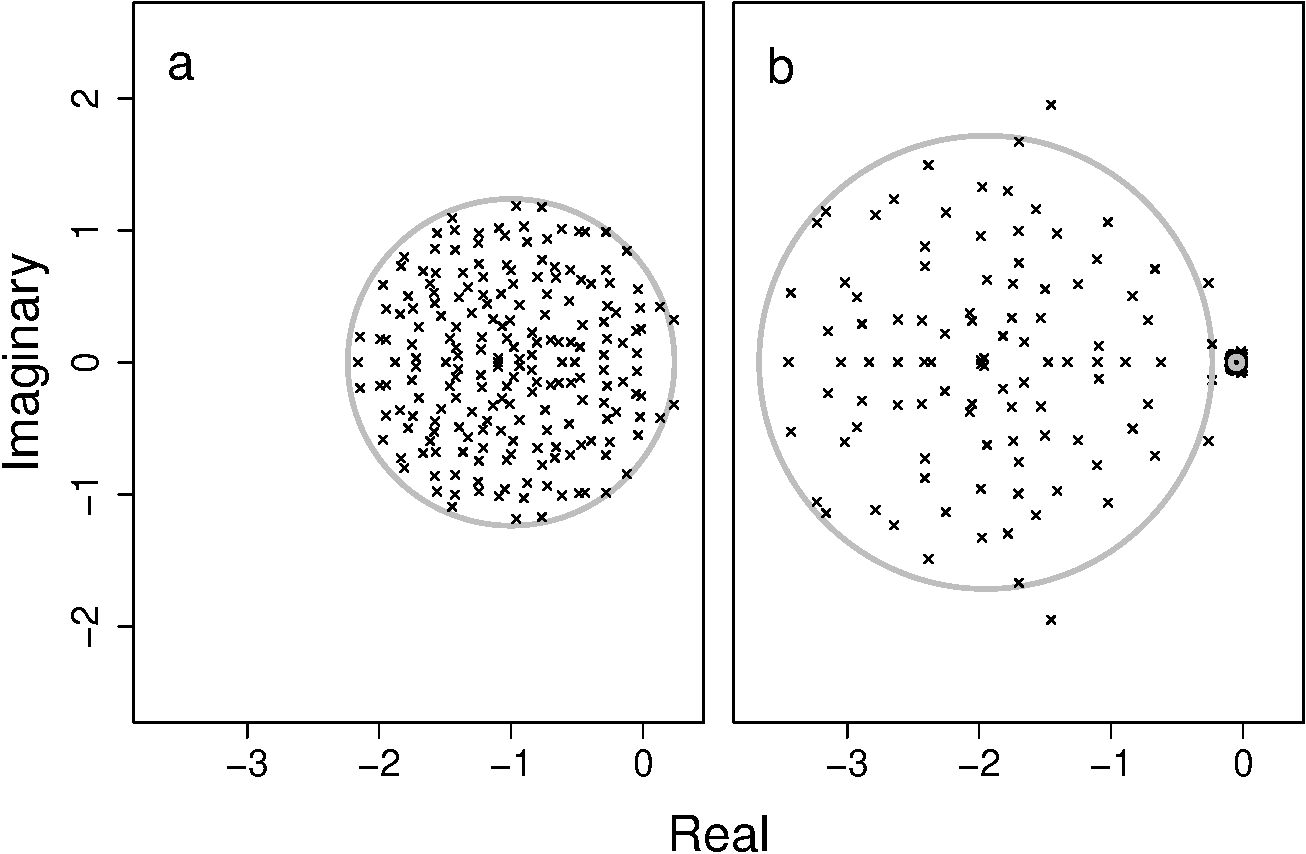
\includegraphics{unnamed-chunk-4-1.pdf}

\begin{center}\rule{0.5\linewidth}{\linethickness}\end{center}

Rows in \(M\) define how a given component \(i\) is affected by other
components of the system, meaning that the rate of component response
time can be modelled by multiplying all row elements by a real scalar
value
\(\gamma_{i}\)\textsuperscript{\protect\hyperlink{ref-Patel2018}{14}} (see 
\hyperlink{SIstart}{Supplementary Information} for details).
The distribution of \(\gamma\) over \(S\) components thereby models the
distribution of component response rates. An instructive example
compares one \(M\) when \(\gamma_{i} = 1\) for all \(i\) in \(S\) to
the same \(M\) when half of \(\gamma_{i} = 1.95\) and half of
\(\gamma_{i} = 0.05\). This models one system in which \(\gamma\) is
invariant and one in which \(\gamma\) varies, but systems are otherwise
identical (note \(E[\gamma_{i}] = 1\) in both cases). I assume
\(S = 200\), \(C = 0.05\), and \(\sigma = 0.4\); diagonal elements are
set to \(-1\) and non-zero off-diagonal elements are drawn randomly from
\(\mathcal{N}(0, \sigma^{2})\). Rows are then multiplied by
\(\gamma_{i}\) to generate \(M\). When \(\gamma_{i} = 1\), eigenvalues
of \(M\) are distributed uniformly within a circle centred at
(\(-1, 0\)) with a radius of 1.265 (Fig. 1a). Hence, the real components
of eigenvalues are highly unlikely to all be negative when all
\(\gamma_{i} = 1\). But when \(\gamma_{i}\) values are separated into
two groups, eigenvalues are no longer uniformly distributed (Fig. 1b).
Instead, two distinct clusters of eigenvalues appear (grey circles in
Fig. 1b), one centred at (\(-1.95, 0\)) and the other centred at
(\(-0.05, 0\)). The former has a large radius, but the real components
have shifted to the left (in comparison to when \(\gamma = 1\)) and all
\(\Re({\lambda}) < 0\). The latter cluster has real components that have
shifted to the right, but has a smaller radius. Overall, for 1 million
randomly assembled \(M\), this division between slow and fast component
response rates results in more stable systems: 1 stable given
\(\gamma = 1\) versus 32 stable given \(\gamma = \{1.95, 0.5\}\).

\begin{center}\rule{0.5\linewidth}{\linethickness}\end{center}

\textbf{Figure 2: Distributions of eigenvalues before (a) and after (b)
introducing variation in component response rate
(\(\boldsymbol{\gamma}\)) in complex systems.} Each panel shows the same
system where \(S = 1000\), \(C = 1\), and \(\sigma = 0.4\). \textbf{a.}
Eigenvalues plotted in the absence of \(Var(\gamma)\) where
\(E[\gamma] = 1\), versus \textbf{b.} eigenvalues plotted given
\(\gamma \sim \mathcal{U}(0, 2)\), which increases the variance of
interaction strengths (\(\sigma^{2}\)) but clusters eigenvalues toward
the distribution's centre (-1, 0). Black and red elipses in both panels
show the circle centred on the distribution in panels a and b,
respectively, which have a radius of \(\sigma \sqrt{SC}\). Proportions
of \(\Re(\lambda) < 0\) are 0.548 and 0.552 for a and b, respectively.

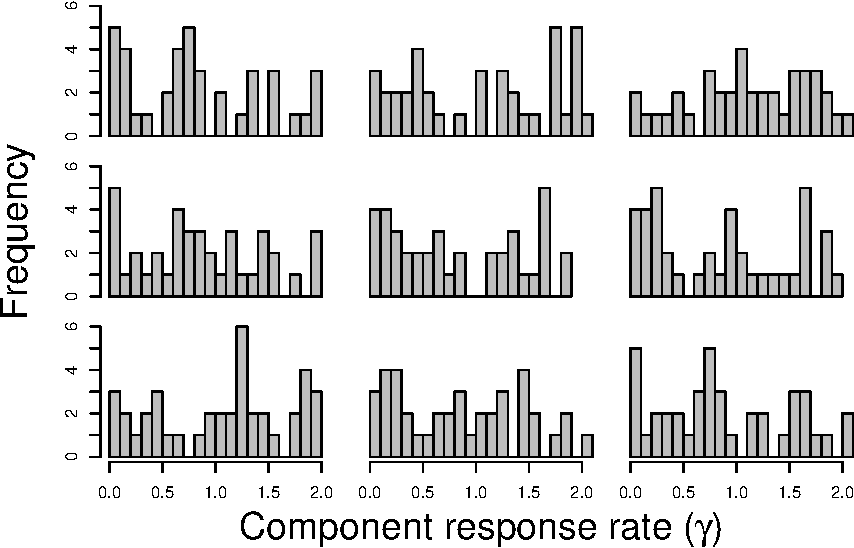
\includegraphics{unnamed-chunk-7-1.pdf}

\begin{center}\rule{0.5\linewidth}{\linethickness}\end{center}

Higher stability in systems with variation in \(\gamma\) can be observed
by sampling \(\gamma_{i}\) values from various distributions. I now
focus on a uniform distribution where \(\gamma \sim \mathcal{U}(0, 2)\)
(see \hyperlink{SIstart}{Supplementary Information} for other distributions, 
which give
similar results). As with the case of \(\gamma = \{1.95, 0.5\}\) (Fig.
1b), \(E[\gamma] = 1\) when \(\gamma \sim \mathcal{U}(0, 2)\), allowing
comparison of \(M\) before and after variation in component response
rate. Figure 2 shows a comparison of eigenvalue distributions given
\(S = 1000\), \(C = 1\), and \(\sigma = 0.4\). As
expected\textsuperscript{\protect\hyperlink{ref-Tao2010}{17}}, when
\(\gamma = 1\), eigenvalues are distributed uniformly in a circle
centred at (\(-1, 0\)) with a radius of \(\sigma\sqrt{SC} =\) 12.649.
Uniform variation in \(\gamma\) leads to a non-uniform distribution of
eigenvalues, some of which are clustered tightly around the centre of
the distribution, but others of which are spread outside the former
radius of 12.649 (red circle Fig 2b). This larger radius occurs because
the addition of \(Var(\gamma)\) increases the realised \(\sigma\) of
\(M\). The clustering and spreading of eigenvalues introduced by
\(Var(\gamma)\) can destabilise previously stable systems or stabilise
systems that are otherwise unstable. But where systems are otherwise too
complex to be stable given \(\gamma = 1\), the effect of \(Var(\gamma)\)
can often lead to stability above
May's\textsuperscript{\protect\hyperlink{ref-May1972}{1},\protect\hyperlink{ref-Allesina2012}{2}}
threshold of \(\sigma\sqrt{SC} > 1\).

\begin{center}\rule{0.5\linewidth}{\linethickness}\end{center}

\textbf{Figure 3: Stability of large complex systems with and without
variation in component response rate(\(\boldsymbol{\gamma}\)).} Y-axes show
the \(\ln\) number of systems that are stable across different system sizes
(\(S\)) given \(C = 1\) (left axis), and the proportion of systems in which
variation in \(\gamma\) is critical for system stability (right axis). For each
\(S\), 1 million complex systems are randomly generated. Stability of
each complex system is tested given variation in \(\gamma\) by randomly
sampling \(\gamma \sim \mathcal{U}(0, 2)\). Stability given
\(Var(\gamma)\) is then compared to stability in an otherwise identical
system in which \(\gamma = E[\mathcal{U}(0, 2)]\) for all components.
Light and dark grey bars show the number of stable systems in the
absence versus presence of \(Var(\gamma)\), respectively. The black line
shows the proportion of systems that are stable when
\(Var(\gamma) > 0\), but would be unstable if \(Var(\gamma) = 0\).

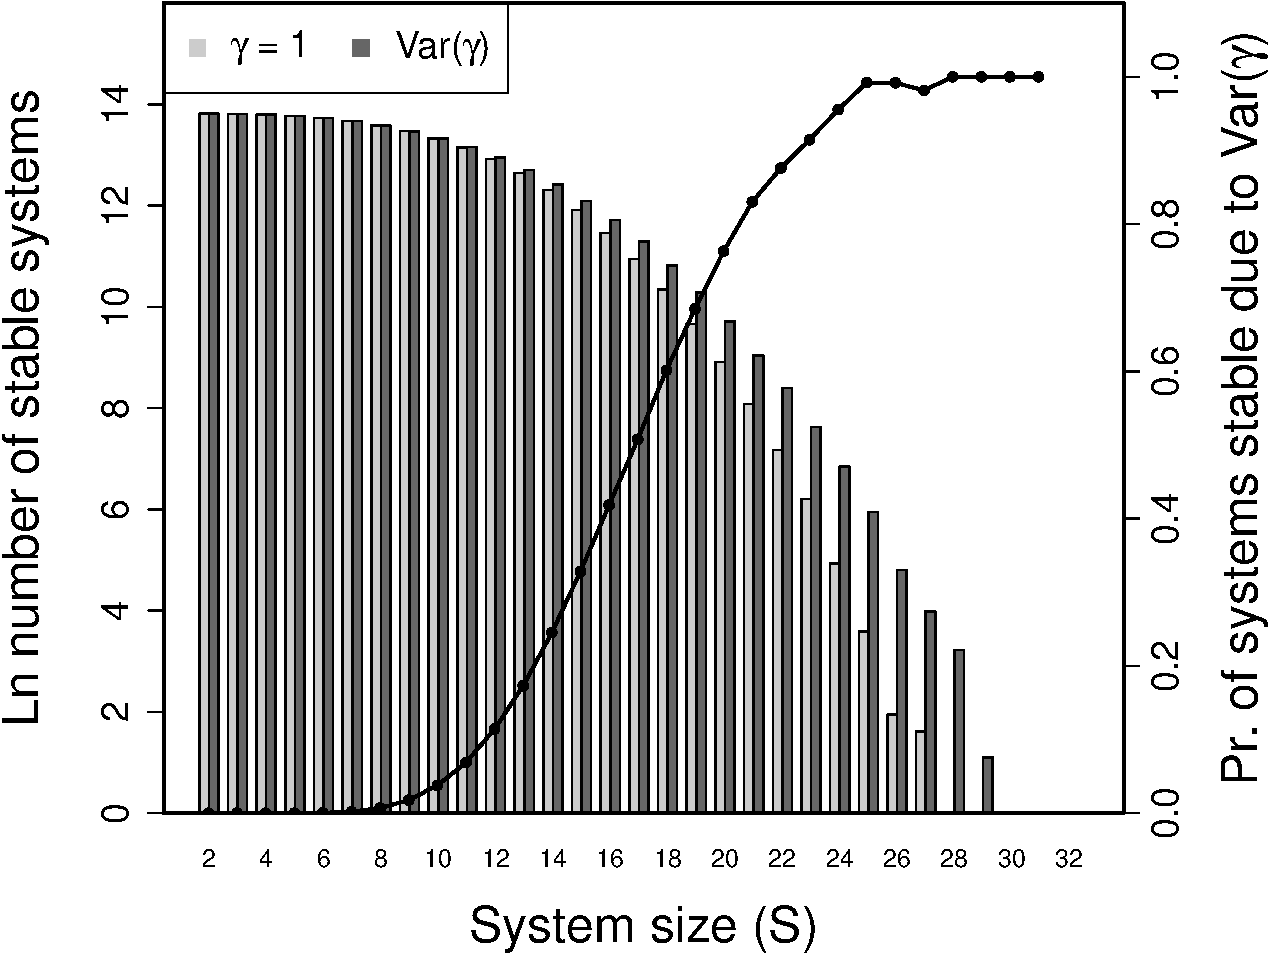
\includegraphics{unnamed-chunk-9-1.pdf}

\begin{center}\rule{0.5\linewidth}{\linethickness}\end{center}

To investigate the effect of \(Var(\gamma)\) on system stability, I
simulated random \(M\) matrices at \(\sigma = 0.4\) and \(C = 1\) across
\(S\) ranging from 2-32. One million \(M\) were simulated 
for each \(S\), and the stability of \(M\) was assessed given \(\gamma = 1\)
versus \(\gamma \sim \mathcal{U}(0, 2)\). I found that the number of stable 
random systems was
consistently higher given \(Var(\gamma)\) than when \(\gamma = 1\) (Fig.
3), and that the difference between the probabilities of observing a
stable system increased with an increase in \(S\); i.e., the potential
for \(Var(\gamma)\) to drive stability increased with system complexity.
For the highest values of \(S\), nearly all systems that were stable
given \(Var(\gamma)\) would not have been stable given \(\gamma = 1\) (see
\hyperlink{SIstart}{Supplementary Information} for full results). This 
suggests that the
stability of large systems might be dependent upon variation in the
response rates of their individual components, meaning that factors such
as generation time (in ecological networks), transaction speed (in
economic networks), or communication speed (in social networks) need to
be considered when investigating the stability of complex systems.

It is important to point out 
that \(Var(\gamma)\) is not stabilising per se; that is,
adding variation in \(\gamma\) to a particular system \(M\) does not
necessarily increase the probability that the system will be stable (see
\hyperlink{SIstart}{Supplementary Information}). Rather, systems that are 
observed to be stable are more likely to vary in \(\gamma\), and for this
\(Var(\gamma)\) to be critical to their stability. This is caused by the
shift in the distribution of eigenvalues that occurs by introducing
\(Var(\gamma)\) (Fig. 1b, 2b), which can sometimes result in all
\(\Re(\lambda) < 0\) but might also increase \(\Re(\lambda)\) values. 

To further investigate the potential of \(Var(\gamma)\) to be stabilising,
I used a genetic algorithm (the space of possible \(\gamma\)
values was too large to search
exhaustively\textsuperscript{\protect\hyperlink{ref-Hamblin2013}{18}};
see \hyperlink{SIstart}{Supplementary Information}). For each of 10000 
random \(M\), the
genetic algorithm initialised 1000 different sets of
\(\gamma \sim \mathcal{U}(0, 2)\) values of size \(S\). Eigenanalysis was
performed on \(M\) using 
each set of \(\gamma\) values, and the 20 sets with the
lowest \(\max\left(\Re(\lambda)\right)\) each produced 50 clonal offspring with
subsequent mutation and crossover between the resulting new population
of 1000 \(\gamma\) sets. The genetic algorithm terminated if a stable
\(M\) was found, 20 generations occurred, or a convergence criteria of
minimum fitness increase between generations was satisfied. Across
\(S = \{2, 3, ..., 39, 40\}\), sets of \(\gamma\) values were found that
resulted in stable systems with probabilities that were up to four orders of
magnitude higher than when \(\gamma = 1\) (see \hyperlink{SIstart}{Supplementary
Information}), meaning that stability could often be achieved by 
manipulating \(S\) \(\gamma\) values rather than \(S \times S\) \(M\) elements.
Hence, managing the response rates of system components in a targetted
way can potentially facilitate the stabilisation of complex systems 
through a reduction in dimensionality.

I have focused broadly on random complex systems, but it is also
worthwhile to consider more restricted interactions such as those of
specific ecological
networks\textsuperscript{\protect\hyperlink{ref-Allesina2012}{2}}. These
include systems in which all interactions are negative (competitive networks), positive (mutualist networks), or \(i\) and
\(j\) pairs have opposing signs (predator-prey networks). In
general, competitive and mutualist networks tend to be destabilising,
and predator-prey networks tend to be
stabilising\textsuperscript{\protect\hyperlink{ref-Allesina2011}{19}}.
When \(Var(\gamma)\) is applied to each, the proportion of stable
competitive and predator-prey networks increases, but the proportion of
stable mutualist networks does not (see 
\hyperlink{SIstart}{Supplementary Information}).
Additionally, when each component of \(M\) is interpreted as a unique
species and given a random intrinsic growth
rate\textsuperscript{\protect\hyperlink{ref-Dougoud2018}{20}},
feasibility is not increased by \(Var(\gamma)\), suggesting that
variation in species generation time might be unlikely to drive
stability in purely multi-species networks (see \hyperlink{SIstart}{Supplementary
Information}).

My results show that complex systems are more likely to be stable when
the response rates of system components vary. These results are broadly
applicable to complex biological and social networks.

\textbf{Acknowledgements}

I am supported by a Leverhulme Trust Early Career Fellowship (ECF-2016-376).
Conversations with L. Bussi\`ere and N. Bunnefeld, and helpful comments from
J. J. Cusack and I. L. Jones, improved the quality of this work. 

\textbf{References}

\hypertarget{refs}{}
\hypertarget{ref-May1972}{}
1. May, R. M. Will a large complex system be stable? \emph{Nature}
\textbf{238,} 413--414 (1972).

\hypertarget{ref-Allesina2012}{}
2. Allesina, S. \& Tang, S. Stability criteria for complex ecosystems.
\emph{Nature} \textbf{483,} 205--208 (2012).

\hypertarget{ref-Gray2008}{}
3. Gray, R. T. \& Robinson, P. A. Stability and synchronization of
random brain networks with a distribution of connection strengths.
\emph{Neurocomputing} \textbf{71,} 1373--1387 (2008).

\hypertarget{ref-Gray2009}{}
4. Gray, R. T. \& Robinson, P. A. Stability of random brain networks
with excitatory and inhibitory connections. \emph{Neurocomputing}
\textbf{72,} 1849--1858 (2009).

\hypertarget{ref-Rosenfeld2009}{}
5. Rosenfeld, S. Patterns of stochastic behavior in dynamically unstable
high-dimensional biochemical networks. \emph{Gene Regulation and Systems
Biology} \textbf{3,} 1--10 (2009).

\hypertarget{ref-MacArthur2010}{}
6. MacArthur, B. D., Sanchez-Garcia, R. J. \& Ma'ayan, A. Microdynamics
and criticality of adaptive regulatory networks. \emph{Physics Review
Letters} \textbf{104,} 168701 (2010).

\hypertarget{ref-Haldane2011}{}
7. Haldane, A. G. \& May, R. M. Systemic risk in banking ecosystems.
\emph{Nature} \textbf{469,} 351--355 (2011).

\hypertarget{ref-Suweis2014}{}
8. Suweis, S. \& D'Odorico, P. Early warning signs in social-ecological
networks. \emph{PLoS ONE} \textbf{9,} (2014).

\hypertarget{ref-Bardoscia2017}{}
9. Bardoscia, M., Battiston, S., Caccioli, F. \& Caldarelli, G. Pathways
towards instability in financial networks. \emph{Nature Communications}
\textbf{8,} 1--7 (2017).

\hypertarget{ref-Mougi2012}{}
10. Mougi, A. \& Kondoh, M. Diversity of interaction types and
ecological community stability. \emph{Science} \textbf{337,} 349--351
(2012).

\hypertarget{ref-Allesina2015a}{}
11. Allesina, S. \& Tang, S. The stability--complexity relationship at
age 40: a random matrix perspective. \emph{Population Ecology} 63--75
(2015).
doi:\href{https://doi.org/10.1007/s10144-014-0471-0}{10.1007/s10144-014-0471-0}

\hypertarget{ref-Gao2016}{}
12. Gao, J., Barzel, B. \& Barabási, A. L. Universal resilience patterns
in complex networks. \emph{Nature} \textbf{530,} 307--312 (2016).

\hypertarget{ref-Grilli2017}{}
13. Grilli, J. \emph{et al.} Feasibility and coexistence of large
ecological communities. \emph{Nature Communications} \textbf{8,} (2017).

\hypertarget{ref-Patel2018}{}
14. Patel, S., Cortez, M. H. \& Schreiber, S. J. Partitioning the
effects of eco-evolutionary feedbacks on community stability.
\emph{American Naturalist} \textbf{191,} 1--29 (2018).

\hypertarget{ref-Allesina2015}{}
15. Allesina, S. \emph{et al.} Predicting the stability of large
structured food webs. \emph{Nature Communications} \textbf{6,} 7842
(2015).

\hypertarget{ref-May2008}{}
16. May, R. M., Levin, S. A. \& Sugihara, G. Complex systems: Ecology
for bankers. \emph{Nature} \textbf{451,} 893--895 (2008).

\hypertarget{ref-Tao2010}{}
17. Tao, T. \& Vu, V. Random matrices: Universality of ESDs and the
circular law. \emph{Annals of Probability} \textbf{38,} 2023--2065
(2010).

\hypertarget{ref-Hamblin2013}{}
18. Hamblin, S. On the practical usage of genetic algorithms in ecology
and evolution. \emph{Methods in Ecology and Evolution} \textbf{4,}
184--194 (2013).

\hypertarget{ref-Allesina2011}{}
19. Allesina, S. \& Levine, J. M. A competitive network theory of
species diversity. \emph{Proceedings of the National Academy of Sciences
of the United States of America} \textbf{108,} 5638--5642 (2011).

\hypertarget{ref-Dougoud2018}{}
20. Dougoud, M., Vinckenbosch, L., Rohr, R., Bersier, L.-F. \& Mazza, C.
The feasibility of equilibria in large ecosystems: a primary but
neglected concept in the complexity-stability debate. \emph{PLOS
Computational Biology} \textbf{14,} e1005988 (2018).

\clearpage

\begin{center}
\hypertarget{SIstart}{\section{Supplementary Information}\label{SIstart}}
\end{center}

\begin{center}\rule{0.5\linewidth}{\linethickness}\end{center}

\textbf{This supplementary information supports the manuscript
``Component response rate variation drives stability in large complex
systems'' with all of the code required to recreate the analysis in the
main text, and with additional analyses to support its conclusions. All
text, code, and data underlying this manuscript are publicly available
on \href{https://github.com/bradduthie/RandomMatrixStability}{GitHub}
as part of the RandomMatrixStability package.}

The
\href{https://github.com/bradduthie/RandomMatrixStability}{RandomMatrixStability
package} includes all functions and tools for recreating the text, this
supplemental information, and running all code; additional documentation
is also provided for functions as part of the package. The
RandomMatrixStability package is available on
\href{https://github.com/bradduthie/RandomMatrixStability}{GitHub}; to
download it, the
\href{https://cran.r-project.org/web/packages/devtools/index.html}{\texttt{devtools}
library} is needed.

\begin{Shaded}
\begin{Highlighting}[]
\KeywordTok{install.packages}\NormalTok{(}\StringTok{"devtools"}\NormalTok{);}
\KeywordTok{library}\NormalTok{(devtools);}
\end{Highlighting}
\end{Shaded}

The code below installs the RandomMatrixStability package using
devtools.

\begin{Shaded}
\begin{Highlighting}[]
\KeywordTok{install_github}\NormalTok{(}\StringTok{"bradduthie/RandomMatrixStability"}\NormalTok{);}
\end{Highlighting}
\end{Shaded}

While downloading this package is recommended, all relevant code is also
reproduced below with explanation, so it is possible to recreate all
analyses using only this Supplementary Information.

\begin{center}\rule{0.5\linewidth}{\linethickness}\end{center}

\section{Supplementary Information table of
contents}\label{supplemental-information-table-of-contents}

\begin{itemize}
\tightlist
\item
  \protect\hyperlink{moregamma}{Further explanation of \(\gamma\)}
\item
  \protect\hyperlink{Fig1}{Code and simulations underlying Fig. 1}
\item
  \protect\hyperlink{Fig2}{Code and simulations underlying Fig. 2}
\item
  \protect\hyperlink{IncrS}{Stability across increasing \(S\)}
\item
  \protect\hyperlink{ecological}{Stability of ecological networks}

  \begin{itemize}
  \tightlist
  \item
    \protect\hyperlink{competition}{Competitor networks}
  \item
    \protect\hyperlink{mutualism}{Mutualist networks}
  \item
    \protect\hyperlink{pred-prey}{Predator-prey networks}
  \end{itemize}
\item
  \protect\hyperlink{connectance}{Different connectance (C) values}

  \begin{itemize}
  \tightlist
  \item
    \protect\hyperlink{connect3}{C = 0.3}
  \item
    \protect\hyperlink{connect5}{C = 0.5}
  \item
    \protect\hyperlink{connect7}{C = 0.7}
  \item
    \protect\hyperlink{connect9}{C = 0.9}
  \end{itemize}
\item
  \protect\hyperlink{gam_dist}{Different distributions of \(\gamma\)}
\item
  \protect\hyperlink{ga}{Genetic algorithm}
\item
  \protect\hyperlink{Feasibility}{Feasibility of complex systems}
\end{itemize}

\hypertarget{moregamma}{\section{\texorpdfstring{Further explanation of
\(\gamma\)}{Further explanation of \textbackslash{}gamma}}\label{moregamma}}

In a synthesis of eco-evolutionary feedbacks on community stability,
Patel et al. model a system that includes a vector of potentially
changing species densities (\(\mathbf{N}\)) and a vector of potentially
evolving traits
(\(\mathbf{x}\))\textsuperscript{\protect\hyperlink{ref-Patel2018}{1}}.
For any species \(i\) or trait \(j\), change in species density
(\(N_{i}\)) or trait value (\(x_{j}\)) with time (\(t\)) is a function
of the vectors \(\mathbf{N}\) and \(\mathbf{x}\),

\[\frac{dN_{i}}{dt} = N_{i}f_{i}(\mathbf{N}, \mathbf{x}),\]

\[\frac{dx_{j}}{dt} = \epsilon g_{j}(\mathbf{N}, \mathbf{x}).\]

In the above, \(f_{i}\) and \(g_{j}\) are functions that define the
effects of all species densities and trait values on the density of a
species \(i\) and the value of trait \(j\), respectively. Patel et al.
were interested in stability when the evolution of traits was relatively
slow or fast in comparison with the change in species
densities\textsuperscript{\protect\hyperlink{ref-Patel2018}{1}}, and
this is modulated in the above by the scalar \(\epsilon\). The value of
\(\epsilon\) thereby determines the timescale separation between ecology
and evolution, with high \(\epsilon\) modelling relatively fast
evolution and low \(\epsilon\) modelling relative slow
evolution\textsuperscript{\protect\hyperlink{ref-Patel2018}{1}}.

I use the same principle that Patel et al. use to modulate the relative
rate of evolution to modulate rates of component responses for \(S\)
components. Following
May\textsuperscript{\protect\hyperlink{ref-May1972}{2},\protect\hyperlink{ref-May1973}{3}},
the value of a component \(i\) at time \(t\) (\(v_{i}(t)\)) is affected
by the value of \(j\) (\(v_{j}(t)\)) and \(j\)'s marginal effect on
\(i\) (\(m_{ij}\)), and by \(i\)'s response rate (\(\gamma_{i}\)),

\[\frac{dv_{i}(t)}{dt} = \gamma_{i} \sum_{j=1}^{S}m_{ij}v_{j}(t).\]

In matrix notation\textsuperscript{\protect\hyperlink{ref-May1973}{3}},

\[\frac{d\mathbf{v}(t)}{dt} = \mathbf{\gamma} \mathbf{M}\mathbf{v}(t).\]

In the above, \(\mathbf{\gamma}\) is a diagonal matrix in which elements
correspond to individual component response rates. Therefore,
\(\mathbf{\gamma} \mathbf{M}\) modulates the values of components and
can be analysed using the techniques of
May\textsuperscript{\protect\hyperlink{ref-May1972}{2},\protect\hyperlink{ref-May1973}{3}}.

\hypertarget{Fig1}{\section{Code and simulations underlying Fig.
1}\label{Fig1}}

The sample \(M\) used for the eigenvalue distributions in Fig. 1 of the
text is available on
\href{https://github.com/bradduthie/RandomMatrixStability/tree/master/notebook/sim_results/bi_gamma}{GitHub},
and was produced by running the following function.

\begin{Shaded}
\begin{Highlighting}[]
\NormalTok{find_bgamma <-}\StringTok{ }\NormalTok{function(}\DataTypeTok{S =} \DecValTok{200}\NormalTok{, }\DataTypeTok{C =} \FloatTok{0.05}\NormalTok{, }\DataTypeTok{Osd =} \FloatTok{0.4}\NormalTok{, }\DataTypeTok{iters =} \DecValTok{10000}\NormalTok{)\{}
    \NormalTok{while(iters >}\StringTok{ }\DecValTok{0}\NormalTok{)\{}
        \NormalTok{A_dat  <-}\StringTok{ }\KeywordTok{rnorm}\NormalTok{(}\DataTypeTok{n =} \NormalTok{S *}\StringTok{ }\NormalTok{S, }\DataTypeTok{mean =} \DecValTok{0}\NormalTok{, }\DataTypeTok{sd =} \NormalTok{Osd);}
        \NormalTok{A_mat  <-}\StringTok{ }\KeywordTok{matrix}\NormalTok{(}\DataTypeTok{data =} \NormalTok{A_dat, }\DataTypeTok{nrow =} \NormalTok{S);}
        \NormalTok{C_dat  <-}\StringTok{ }\KeywordTok{rbinom}\NormalTok{(}\DataTypeTok{n =} \NormalTok{S *}\StringTok{ }\NormalTok{S, }\DataTypeTok{size =} \DecValTok{1}\NormalTok{, }\DataTypeTok{prob =} \NormalTok{C);}
        \NormalTok{C_mat  <-}\StringTok{ }\KeywordTok{matrix}\NormalTok{(}\DataTypeTok{data =} \NormalTok{C_dat, }\DataTypeTok{nrow =} \NormalTok{S, }\DataTypeTok{ncol =} \NormalTok{S);}
        \NormalTok{A_mat  <-}\StringTok{ }\NormalTok{A_mat *}\StringTok{ }\NormalTok{C_mat;}
        \NormalTok{gammas <-}\StringTok{ }\KeywordTok{c}\NormalTok{(}\KeywordTok{rep}\NormalTok{(}\FloatTok{1.95}\NormalTok{, S/}\DecValTok{2}\NormalTok{), }\KeywordTok{rep}\NormalTok{(}\FloatTok{0.05}\NormalTok{, S/}\DecValTok{2}\NormalTok{))}
        \NormalTok{mu_gam <-}\StringTok{ }\KeywordTok{mean}\NormalTok{(gammas);}
        \KeywordTok{diag}\NormalTok{(A_mat) <-}\StringTok{ }\NormalTok{-}\DecValTok{1}\NormalTok{;}
        \NormalTok{A1     <-}\StringTok{ }\NormalTok{gammas *}\StringTok{ }\NormalTok{A_mat;}
        \NormalTok{A0     <-}\StringTok{ }\NormalTok{mu_gam *}\StringTok{ }\NormalTok{A_mat;}
        \NormalTok{A0_e   <-}\StringTok{ }\KeywordTok{eigen}\NormalTok{(A0)$values;}
        \NormalTok{A0_r   <-}\StringTok{ }\KeywordTok{Re}\NormalTok{(A0_e);}
        \NormalTok{A0_i   <-}\StringTok{ }\KeywordTok{Im}\NormalTok{(A0_e);}
        \NormalTok{A1_e   <-}\StringTok{ }\KeywordTok{eigen}\NormalTok{(A1)$values;}
        \NormalTok{A1_r   <-}\StringTok{ }\KeywordTok{Re}\NormalTok{(A1_e);}
        \NormalTok{A1_i   <-}\StringTok{ }\KeywordTok{Im}\NormalTok{(A1_e);}
        \NormalTok{if(}\KeywordTok{max}\NormalTok{(A0_r) >=}\StringTok{ }\DecValTok{0} \NormalTok{&}\StringTok{ }\KeywordTok{max}\NormalTok{(A1_r) <}\StringTok{ }\DecValTok{0}\NormalTok{)\{}
            \KeywordTok{return}\NormalTok{(}\KeywordTok{list}\NormalTok{(}\DataTypeTok{A0 =} \NormalTok{A0, }\DataTypeTok{A1 =} \NormalTok{A1));}
            \NormalTok{break;}
        \NormalTok{\}}
        \KeywordTok{print}\NormalTok{(iters);}
        \NormalTok{iters <-}\StringTok{ }\NormalTok{iters -}\StringTok{ }\DecValTok{1}\NormalTok{;}
    \NormalTok{\}}
\NormalTok{\}}
\end{Highlighting}
\end{Shaded}

The above \texttt{find\_bgamma} function terminates when a matrix \(M\)
is found that is not stable when all component response rates are set to
\(\gamma = 1\), but is stable when half of component response rates are
\(1.95\) and half are \(0.05\). The function is used to illustrate the
concept of how fast versus slow component responses can cause a system
to become stable. Simulations were run for \texttt{iter\ =\ 1000000},
but terminated once an acceptable \texttt{A0} and \texttt{A1} were
found. The code below plots the eigenvalue distributions of \texttt{A0}
and \texttt{A1} in panels \textbf{a} and \textbf{b}, respectively. The
plot itself can be recreated with the function and code below.

\begin{Shaded}
\begin{Highlighting}[]
\NormalTok{A0 <-}\StringTok{ }\KeywordTok{as.matrix}\NormalTok{(A0[,-}\DecValTok{1}\NormalTok{]);}
\NormalTok{A1 <-}\StringTok{ }\KeywordTok{as.matrix}\NormalTok{(A1[,-}\DecValTok{1}\NormalTok{]);}
\NormalTok{plot_Fig_1 <-}\StringTok{ }\NormalTok{function(A0, A1)\{}
    \NormalTok{S_val       <-}\StringTok{ }\KeywordTok{dim}\NormalTok{(A0)[}\DecValTok{1}\NormalTok{];}
    \NormalTok{A0_e        <-}\StringTok{ }\KeywordTok{eigen}\NormalTok{(A0)$values;}
    \NormalTok{A0_r        <-}\StringTok{ }\KeywordTok{Re}\NormalTok{(A0_e);}
    \NormalTok{A0_i        <-}\StringTok{ }\KeywordTok{Im}\NormalTok{(A0_e);}
    \NormalTok{A1_e        <-}\StringTok{ }\KeywordTok{eigen}\NormalTok{(A1)$values;}
    \NormalTok{A1_r        <-}\StringTok{ }\KeywordTok{Re}\NormalTok{(A1_e);}
    \NormalTok{A1_i        <-}\StringTok{ }\KeywordTok{Im}\NormalTok{(A1_e);}
    \NormalTok{A0_vm       <-}\StringTok{ }\NormalTok{A0;}
    \KeywordTok{diag}\NormalTok{(A0_vm) <-}\StringTok{ }\OtherTok{NA}\NormalTok{;}
    \NormalTok{A0vec       <-}\StringTok{ }\KeywordTok{as.vector}\NormalTok{(}\KeywordTok{t}\NormalTok{(A0_vm));}
    \NormalTok{A0vec       <-}\StringTok{ }\NormalTok{A0vec[}\KeywordTok{is.na}\NormalTok{(A0vec) ==}\StringTok{ }\OtherTok{FALSE}\NormalTok{];}
    \NormalTok{A1_vm       <-}\StringTok{ }\NormalTok{A1;}
    \KeywordTok{diag}\NormalTok{(A1_vm) <-}\StringTok{ }\OtherTok{NA}\NormalTok{;}
    \NormalTok{A1vec       <-}\StringTok{ }\KeywordTok{as.vector}\NormalTok{(}\KeywordTok{t}\NormalTok{(A1_vm));}
    \NormalTok{A1vec       <-}\StringTok{ }\NormalTok{A1vec[}\KeywordTok{is.na}\NormalTok{(A1vec) ==}\StringTok{ }\OtherTok{FALSE}\NormalTok{];}
    \NormalTok{fhalf       <-}\StringTok{ }\DecValTok{1}\NormalTok{:(}\FloatTok{0.5}\NormalTok{*}\KeywordTok{length}\NormalTok{(A1vec));}
    \NormalTok{shalf       <-}\StringTok{ }\NormalTok{(}\FloatTok{0.5}\NormalTok{*}\KeywordTok{length}\NormalTok{(A1vec)+}\DecValTok{1}\NormalTok{):}\KeywordTok{length}\NormalTok{(A1vec);}
    \KeywordTok{par}\NormalTok{(}\DataTypeTok{mfrow =} \KeywordTok{c}\NormalTok{(}\DecValTok{1}\NormalTok{, }\DecValTok{2}\NormalTok{), }\DataTypeTok{mar =} \KeywordTok{c}\NormalTok{(}\FloatTok{0.5}\NormalTok{, }\FloatTok{0.5}\NormalTok{, }\FloatTok{0.5}\NormalTok{, }\FloatTok{0.5}\NormalTok{), }\DataTypeTok{oma =} \KeywordTok{c}\NormalTok{(}\DecValTok{5}\NormalTok{, }\DecValTok{5}\NormalTok{, }\DecValTok{0}\NormalTok{, }\DecValTok{0}\NormalTok{));}
    \KeywordTok{plot}\NormalTok{(A0_r, A0_i, }\DataTypeTok{xlim =} \KeywordTok{c}\NormalTok{(-}\FloatTok{3.7}\NormalTok{, }\FloatTok{0.3}\NormalTok{), }\DataTypeTok{ylim =} \KeywordTok{c}\NormalTok{(-}\DecValTok{2}\NormalTok{, }\DecValTok{2}\NormalTok{), }\DataTypeTok{pch =} \DecValTok{4}\NormalTok{, }\DataTypeTok{cex =} \FloatTok{0.7}\NormalTok{,}
         \DataTypeTok{xlab =} \StringTok{""}\NormalTok{, }\DataTypeTok{ylab =} \StringTok{""}\NormalTok{, }\DataTypeTok{cex.lab =} \FloatTok{1.5}\NormalTok{, }\DataTypeTok{cex.axis =} \FloatTok{1.5}\NormalTok{, }\DataTypeTok{asp =} \DecValTok{1}\NormalTok{);}
    \NormalTok{vl   <-}\StringTok{ }\KeywordTok{seq}\NormalTok{(}\DataTypeTok{from =} \DecValTok{0}\NormalTok{, }\DataTypeTok{to =} \DecValTok{2}\NormalTok{*pi, }\DataTypeTok{by =} \FloatTok{0.001}\NormalTok{);}
    \NormalTok{A0x0 <-}\StringTok{ }\KeywordTok{sqrt}\NormalTok{(S_val) *}\StringTok{ }\KeywordTok{sd}\NormalTok{(A0vec) *}\StringTok{ }\KeywordTok{cos}\NormalTok{(vl) +}\StringTok{ }\KeywordTok{mean}\NormalTok{(}\KeywordTok{diag}\NormalTok{(A0));}
    \NormalTok{A0y0 <-}\StringTok{ }\KeywordTok{sqrt}\NormalTok{(S_val) *}\StringTok{ }\KeywordTok{sd}\NormalTok{(A0vec) *}\StringTok{ }\KeywordTok{sin}\NormalTok{(vl);}
    \KeywordTok{text}\NormalTok{(}\DataTypeTok{x =} \NormalTok{-}\FloatTok{3.5}\NormalTok{, }\DataTypeTok{y =} \FloatTok{2.25}\NormalTok{, }\DataTypeTok{labels =} \StringTok{"a"}\NormalTok{, }\DataTypeTok{cex =} \DecValTok{2}\NormalTok{);}
    \KeywordTok{points}\NormalTok{(}\DataTypeTok{x =} \NormalTok{A0x0, }\DataTypeTok{y =} \NormalTok{A0y0, }\DataTypeTok{type =} \StringTok{"l"}\NormalTok{, }\DataTypeTok{lwd =} \DecValTok{3}\NormalTok{, }\DataTypeTok{col =} \StringTok{"grey"}\NormalTok{);}
    \KeywordTok{points}\NormalTok{(A0_r, A0_i, }\DataTypeTok{pch =} \DecValTok{4}\NormalTok{, }\DataTypeTok{cex =} \FloatTok{0.7}\NormalTok{);}
    \KeywordTok{plot}\NormalTok{(A1_r, A1_i, }\DataTypeTok{xlim =} \KeywordTok{c}\NormalTok{(-}\FloatTok{3.7}\NormalTok{, }\FloatTok{0.3}\NormalTok{), }\DataTypeTok{ylim =} \KeywordTok{c}\NormalTok{(-}\DecValTok{2}\NormalTok{, }\DecValTok{2}\NormalTok{), }\DataTypeTok{pch =} \DecValTok{4}\NormalTok{, }\DataTypeTok{cex =} \FloatTok{0.7}\NormalTok{,}
         \DataTypeTok{xlab =} \StringTok{""}\NormalTok{, }\DataTypeTok{ylab =} \StringTok{""}\NormalTok{, }\DataTypeTok{cex.lab =} \FloatTok{1.5}\NormalTok{, }\DataTypeTok{cex.axis =} \FloatTok{1.5}\NormalTok{, }\DataTypeTok{asp =} \DecValTok{1}\NormalTok{, }
         \DataTypeTok{col =} \StringTok{"black"}\NormalTok{, }\DataTypeTok{yaxt =} \StringTok{"n"}\NormalTok{);}
    \NormalTok{vl <-}\StringTok{ }\KeywordTok{seq}\NormalTok{(}\DataTypeTok{from =} \DecValTok{0}\NormalTok{, }\DataTypeTok{to =} \DecValTok{2}\NormalTok{*pi, }\DataTypeTok{by =} \FloatTok{0.001}\NormalTok{);}
    \NormalTok{A0x1a <-}\StringTok{ }\KeywordTok{sqrt}\NormalTok{(}\FloatTok{0.5}\NormalTok{*S_val) *}\StringTok{ }\KeywordTok{sd}\NormalTok{(A1vec[fhalf]) *}\StringTok{ }\KeywordTok{cos}\NormalTok{(vl) +}\StringTok{ }\KeywordTok{mean}\NormalTok{(}\KeywordTok{diag}\NormalTok{(A1)[}\DecValTok{1}\NormalTok{:(}\FloatTok{0.5}\NormalTok{*S_val)]);}
    \NormalTok{A0y1a <-}\StringTok{ }\KeywordTok{sqrt}\NormalTok{(S_val) *}\StringTok{ }\KeywordTok{sd}\NormalTok{(A1vec[fhalf]) *}\StringTok{ }\KeywordTok{sin}\NormalTok{(vl);}
    \KeywordTok{points}\NormalTok{(}\DataTypeTok{x =} \NormalTok{A0x1a, }\DataTypeTok{y =} \NormalTok{A0y1a, }\DataTypeTok{type =} \StringTok{"l"}\NormalTok{, }\DataTypeTok{lwd =} \DecValTok{3}\NormalTok{, }\DataTypeTok{col =} \StringTok{"grey"}\NormalTok{);}
    \NormalTok{A0x1b <-}\StringTok{ }\KeywordTok{sqrt}\NormalTok{(}\FloatTok{0.5}\NormalTok{*S_val) *}\StringTok{ }\KeywordTok{sd}\NormalTok{(A1vec[shalf]) *}\StringTok{ }\KeywordTok{cos}\NormalTok{(vl) +}\StringTok{ }
\StringTok{                  }\KeywordTok{mean}\NormalTok{( }\KeywordTok{diag}\NormalTok{(A1)[( (}\FloatTok{0.5}\NormalTok{*S_val) +}\StringTok{ }\DecValTok{1} \NormalTok{):S_val] );}
    \NormalTok{A0y1b <-}\StringTok{ }\KeywordTok{sqrt}\NormalTok{(}\FloatTok{0.5}\NormalTok{*S_val) *}\StringTok{ }\KeywordTok{sd}\NormalTok{(A1vec[shalf]) *}\StringTok{ }\KeywordTok{sin}\NormalTok{(vl);}
    \KeywordTok{points}\NormalTok{(}\DataTypeTok{x =} \NormalTok{A0x1b, }\DataTypeTok{y =} \NormalTok{A0y1b, }\DataTypeTok{type =} \StringTok{"l"}\NormalTok{, }\DataTypeTok{lwd =} \DecValTok{3}\NormalTok{, }\DataTypeTok{col =} \StringTok{"grey"}\NormalTok{);}
    \KeywordTok{points}\NormalTok{(A1_r[}\DecValTok{1}\NormalTok{:S_val], A1_i[}\DecValTok{1}\NormalTok{:S_val],}\DataTypeTok{pch =} \DecValTok{4}\NormalTok{, }\DataTypeTok{cex =} \FloatTok{0.7}\NormalTok{);   }
    \KeywordTok{text}\NormalTok{(}\DataTypeTok{x =} \NormalTok{-}\FloatTok{3.5}\NormalTok{, }\DataTypeTok{y =} \FloatTok{2.25}\NormalTok{, }\DataTypeTok{labels =} \StringTok{"b"}\NormalTok{, }\DataTypeTok{cex =} \DecValTok{2}\NormalTok{);}
    \KeywordTok{mtext}\NormalTok{(}\DataTypeTok{side =} \DecValTok{1}\NormalTok{, }\StringTok{"Real"}\NormalTok{, }\DataTypeTok{outer =} \OtherTok{TRUE}\NormalTok{, }\DataTypeTok{line =} \DecValTok{3}\NormalTok{, }\DataTypeTok{cex =} \DecValTok{2}\NormalTok{);}
    \KeywordTok{mtext}\NormalTok{(}\DataTypeTok{side =} \DecValTok{2}\NormalTok{, }\StringTok{"Imaginary"}\NormalTok{, }\DataTypeTok{outer =} \OtherTok{TRUE}\NormalTok{, }\DataTypeTok{line =} \FloatTok{2.5}\NormalTok{, }\DataTypeTok{cex =} \DecValTok{2}\NormalTok{);}
\NormalTok{\}}
\KeywordTok{plot_Fig_1}\NormalTok{(}\DataTypeTok{A0 =} \NormalTok{A0, }\DataTypeTok{A1 =} \NormalTok{A1);}
\end{Highlighting}
\end{Shaded}

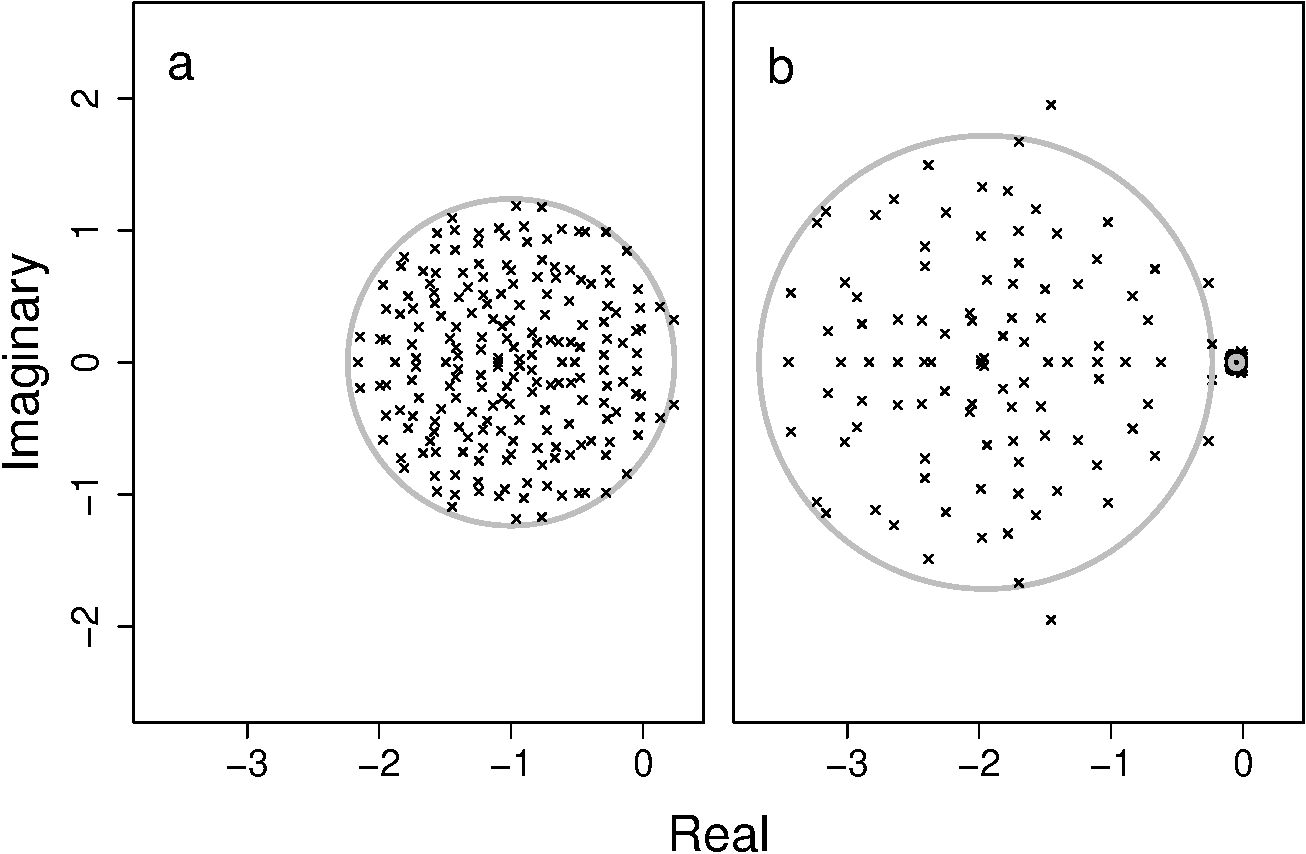
\includegraphics{unnamed-chunk-4-1.pdf}

To find out how frequently \(M\) was stable given that all
\(\gamma = 1\) versus \(\gamma = \{1.95, 0.05\}\), the function below
was created.

\begin{Shaded}
\begin{Highlighting}[]
\NormalTok{stab_bgamma <-}\StringTok{ }\NormalTok{function(}\DataTypeTok{S =} \DecValTok{200}\NormalTok{, }\DataTypeTok{C =} \FloatTok{0.05}\NormalTok{, }\DataTypeTok{Osd =} \FloatTok{0.4}\NormalTok{, }\DataTypeTok{iters =} \DecValTok{10000}\NormalTok{)\{}
    \NormalTok{ress     <-}\StringTok{ }\KeywordTok{matrix}\NormalTok{(}\DataTypeTok{data =} \DecValTok{0}\NormalTok{, }\DataTypeTok{nrow =} \NormalTok{iters, }\DataTypeTok{ncol =} \DecValTok{2}\NormalTok{);}
    \NormalTok{A0_count <-}\StringTok{ }\DecValTok{0}\NormalTok{;}
    \NormalTok{A1_count <-}\StringTok{ }\DecValTok{0}\NormalTok{;}
    \NormalTok{while(iters >}\StringTok{ }\DecValTok{0}\NormalTok{)\{}
        \NormalTok{A_dat  <-}\StringTok{ }\KeywordTok{rnorm}\NormalTok{(}\DataTypeTok{n =} \NormalTok{S *}\StringTok{ }\NormalTok{S, }\DataTypeTok{mean =} \DecValTok{0}\NormalTok{, }\DataTypeTok{sd =} \NormalTok{Osd);}
        \NormalTok{A_mat  <-}\StringTok{ }\KeywordTok{matrix}\NormalTok{(}\DataTypeTok{data =} \NormalTok{A_dat, }\DataTypeTok{nrow =} \NormalTok{S);}
        \NormalTok{C_dat  <-}\StringTok{ }\KeywordTok{rbinom}\NormalTok{(}\DataTypeTok{n =} \NormalTok{S *}\StringTok{ }\NormalTok{S, }\DataTypeTok{size =} \DecValTok{1}\NormalTok{, }\DataTypeTok{prob =} \NormalTok{C);}
        \NormalTok{C_mat  <-}\StringTok{ }\KeywordTok{matrix}\NormalTok{(}\DataTypeTok{data =} \NormalTok{C_dat, }\DataTypeTok{nrow =} \NormalTok{S, }\DataTypeTok{ncol =} \NormalTok{S);}
        \NormalTok{A_mat  <-}\StringTok{ }\NormalTok{A_mat *}\StringTok{ }\NormalTok{C_mat;}
        \NormalTok{gammas <-}\StringTok{ }\KeywordTok{c}\NormalTok{(}\KeywordTok{rep}\NormalTok{(}\FloatTok{1.95}\NormalTok{, S/}\DecValTok{2}\NormalTok{), }\KeywordTok{rep}\NormalTok{(}\FloatTok{0.05}\NormalTok{, S/}\DecValTok{2}\NormalTok{))}
        \NormalTok{mu_gam <-}\StringTok{ }\KeywordTok{mean}\NormalTok{(gammas);}
        \KeywordTok{diag}\NormalTok{(A_mat) <-}\StringTok{ }\NormalTok{-}\DecValTok{1}\NormalTok{;}
        \NormalTok{A1     <-}\StringTok{ }\NormalTok{gammas *}\StringTok{ }\NormalTok{A_mat;}
        \NormalTok{A0     <-}\StringTok{ }\NormalTok{mu_gam *}\StringTok{ }\NormalTok{A_mat;}
        \NormalTok{A0_e   <-}\StringTok{ }\KeywordTok{eigen}\NormalTok{(A0)$values;}
        \NormalTok{A0_r   <-}\StringTok{ }\KeywordTok{Re}\NormalTok{(A0_e);}
        \NormalTok{A0_i   <-}\StringTok{ }\KeywordTok{Im}\NormalTok{(A0_e);}
        \NormalTok{A1_e   <-}\StringTok{ }\KeywordTok{eigen}\NormalTok{(A1)$values;}
        \NormalTok{A1_r   <-}\StringTok{ }\KeywordTok{Re}\NormalTok{(A1_e);}
        \NormalTok{A1_i   <-}\StringTok{ }\KeywordTok{Im}\NormalTok{(A1_e);}
        \NormalTok{if(}\KeywordTok{max}\NormalTok{(A0_r) <}\StringTok{ }\DecValTok{0}\NormalTok{)\{}
            \NormalTok{ress[iters, }\DecValTok{1}\NormalTok{] <-}\StringTok{ }\DecValTok{1}\NormalTok{;}
            \NormalTok{A0_count       <-}\StringTok{ }\NormalTok{A0_count +}\StringTok{ }\DecValTok{1}\NormalTok{;}
            \NormalTok{\}}
        \NormalTok{if(}\KeywordTok{max}\NormalTok{(A1_r) <}\StringTok{ }\DecValTok{0}\NormalTok{)\{}
            \NormalTok{ress[iters, }\DecValTok{2}\NormalTok{] <-}\StringTok{ }\DecValTok{1}\NormalTok{;}
            \NormalTok{A1_count       <-}\StringTok{ }\NormalTok{A1_count +}\StringTok{ }\DecValTok{1}\NormalTok{;}
        \NormalTok{\}}
        \KeywordTok{print}\NormalTok{(}\KeywordTok{c}\NormalTok{(iters, A0_count, A1_count));}
        \NormalTok{iters <-}\StringTok{ }\NormalTok{iters -}\StringTok{ }\DecValTok{1}\NormalTok{;}
    \NormalTok{\}}
    \KeywordTok{return}\NormalTok{(ress);}
\NormalTok{\}}
\end{Highlighting}
\end{Shaded}

The above functions produced the \texttt{bi\_pr\_st} data.

\begin{Shaded}
\begin{Highlighting}[]
\NormalTok{bi_pr_st <-}\StringTok{ }\KeywordTok{read.csv}\NormalTok{(}\StringTok{"sim_results/bi_gamma/bi_pr_st.csv"}\NormalTok{);}
\NormalTok{pr_st    <-}\StringTok{ }\NormalTok{bi_pr_st[,-}\DecValTok{1}\NormalTok{];}
\end{Highlighting}
\end{Shaded}

The function \texttt{stab\_bgamma} was run for
\texttt{iters\ =\ 1000000}, and the resulting matrix \texttt{ress} was
returned. Each row of \texttt{ress} represents a single \(M\) given
\(\gamma = 1\) (column 1) versus \(\gamma = \{1.95, 0.05\}\) (column 2).
Values of 0 indicate that \(M\) was found to be unstable (at least one
real component of its eigenvalues greater than or equal to zero),
whereas values of 1 indicate that \(M\) was found to be stable (all real
components of eigenvalues are negative). The frequencies of stable \(M\)
were 1 given \(\gamma = 1\) and 32 given \(\gamma = \{1.95, 0.05\}\), as
reported in the main text and legend of Fig. 1 (raw data are
\href{https://github.com/bradduthie/RandomMatrixStability/blob/master/notebook/sim_results/bi_gamma/bi_pr_st.csv}{available
on GitHub}).

\hypertarget{Fig2}{\section{Code and simulations underlying Fig.
2}\label{Fig2}}

Figure 2 of the main text shows eigenvalue distributions in a system
where \(S = 1000\), \(C = 1\), and \(\sigma = 0.4\). Eigenvalues can be
reproduced using the code below for when \(\gamma = 1\) (panel a) and
\(\gamma \sim \mathcal{U}(0, 2)\) (panel b). The function below
reproduces the figure.

\begin{Shaded}
\begin{Highlighting}[]
\NormalTok{plot_Fig_2 <-}\StringTok{ }\NormalTok{function()\{}
    \NormalTok{A_comp <-}\StringTok{ }\OtherTok{NULL}\NormalTok{;}
    \NormalTok{A_dat  <-}\StringTok{ }\KeywordTok{rnorm}\NormalTok{(}\DataTypeTok{n =} \DecValTok{1000000}\NormalTok{, }\DataTypeTok{mean =} \DecValTok{0}\NormalTok{, }\DataTypeTok{sd =} \FloatTok{0.4}\NormalTok{);}
    \NormalTok{A_mat  <-}\StringTok{ }\KeywordTok{matrix}\NormalTok{(}\DataTypeTok{data =} \NormalTok{A_dat, }\DataTypeTok{nrow =} \DecValTok{1000}\NormalTok{);}
    \NormalTok{C_dat  <-}\StringTok{ }\KeywordTok{rbinom}\NormalTok{(}\DataTypeTok{n =} \DecValTok{1000} \NormalTok{*}\StringTok{ }\DecValTok{1000}\NormalTok{, }\DataTypeTok{size =} \DecValTok{1}\NormalTok{, }\DataTypeTok{prob =} \DecValTok{1}\NormalTok{);}
    \NormalTok{C_mat  <-}\StringTok{ }\KeywordTok{matrix}\NormalTok{(}\DataTypeTok{data =} \NormalTok{C_dat, }\DataTypeTok{nrow =} \DecValTok{1000}\NormalTok{, }\DataTypeTok{ncol =} \DecValTok{1000}\NormalTok{);}
    \NormalTok{A_mat     <-}\StringTok{ }\NormalTok{A_mat *}\StringTok{ }\NormalTok{C_mat;}
    \NormalTok{gammas <-}\StringTok{ }\KeywordTok{runif}\NormalTok{(}\DataTypeTok{n =} \DecValTok{1000}\NormalTok{, }\DataTypeTok{min =} \DecValTok{0}\NormalTok{, }\DataTypeTok{max =} \DecValTok{2}\NormalTok{);}
    \NormalTok{mu_gam <-}\StringTok{ }\KeywordTok{mean}\NormalTok{(gammas);}
    \KeywordTok{diag}\NormalTok{(A_mat) <-}\StringTok{ }\NormalTok{-}\DecValTok{1}\NormalTok{;}
    \NormalTok{A1     <-}\StringTok{ }\NormalTok{gammas *}\StringTok{ }\NormalTok{A_mat;}
    \NormalTok{A0     <-}\StringTok{ }\NormalTok{mu_gam *}\StringTok{ }\NormalTok{A_mat;}
    \NormalTok{A0_e   <-}\StringTok{ }\KeywordTok{eigen}\NormalTok{(A0)$values;}
    \NormalTok{A0_r   <-}\StringTok{ }\KeywordTok{Re}\NormalTok{(A0_e);}
    \NormalTok{A0_i   <-}\StringTok{ }\KeywordTok{Im}\NormalTok{(A0_e);}
    \NormalTok{A1_e   <-}\StringTok{ }\KeywordTok{eigen}\NormalTok{(A1)$values;}
    \NormalTok{A1_r   <-}\StringTok{ }\KeywordTok{Re}\NormalTok{(A1_e);}
    \NormalTok{A1_i   <-}\StringTok{ }\KeywordTok{Im}\NormalTok{(A1_e);}
    \NormalTok{A0_vm       <-}\StringTok{ }\NormalTok{A0;}
    \KeywordTok{diag}\NormalTok{(A0_vm) <-}\StringTok{ }\OtherTok{NA}\NormalTok{;}
    \NormalTok{A0vec       <-}\StringTok{ }\KeywordTok{as.vector}\NormalTok{(A0_vm);}
    \NormalTok{A0vec       <-}\StringTok{ }\NormalTok{A0vec[}\KeywordTok{is.na}\NormalTok{(A0vec) ==}\StringTok{ }\OtherTok{FALSE}\NormalTok{];}
    \NormalTok{A1_vm       <-}\StringTok{ }\NormalTok{A1;}
    \KeywordTok{diag}\NormalTok{(A1_vm) <-}\StringTok{ }\OtherTok{NA}\NormalTok{;}
    \NormalTok{A1vec       <-}\StringTok{ }\KeywordTok{as.vector}\NormalTok{(A1_vm);}
    \NormalTok{A1vec       <-}\StringTok{ }\NormalTok{A1vec[}\KeywordTok{is.na}\NormalTok{(A1vec) ==}\StringTok{ }\OtherTok{FALSE}\NormalTok{];}
    \KeywordTok{par}\NormalTok{(}\DataTypeTok{mfrow =} \KeywordTok{c}\NormalTok{(}\DecValTok{1}\NormalTok{, }\DecValTok{2}\NormalTok{), }\DataTypeTok{mar =} \KeywordTok{c}\NormalTok{(}\FloatTok{0.5}\NormalTok{, }\FloatTok{0.5}\NormalTok{, }\FloatTok{0.5}\NormalTok{, }\FloatTok{0.5}\NormalTok{), }\DataTypeTok{oma =} \KeywordTok{c}\NormalTok{(}\DecValTok{5}\NormalTok{, }\DecValTok{5}\NormalTok{, }\DecValTok{0}\NormalTok{, }\DecValTok{0}\NormalTok{));}
    \KeywordTok{plot}\NormalTok{(A0_r, A0_i, }\DataTypeTok{xlim =} \KeywordTok{c}\NormalTok{(-}\FloatTok{16.5}\NormalTok{, }\FloatTok{15.5}\NormalTok{), }\DataTypeTok{ylim =} \KeywordTok{c}\NormalTok{(-}\FloatTok{16.5}\NormalTok{,}\FloatTok{15.5}\NormalTok{), }\DataTypeTok{pch =} \DecValTok{4}\NormalTok{, }
         \DataTypeTok{cex =} \FloatTok{0.7}\NormalTok{, }\DataTypeTok{xlab =} \StringTok{""}\NormalTok{, }\DataTypeTok{ylab =} \StringTok{""}\NormalTok{, }\DataTypeTok{cex.lab =} \FloatTok{1.5}\NormalTok{, }\DataTypeTok{cex.axis =} \FloatTok{1.5}\NormalTok{, }
         \DataTypeTok{asp =} \DecValTok{1}\NormalTok{);}
    \NormalTok{vl <-}\StringTok{ }\KeywordTok{seq}\NormalTok{(}\DataTypeTok{from =} \DecValTok{0}\NormalTok{, }\DataTypeTok{to =} \DecValTok{2}\NormalTok{*pi, }\DataTypeTok{by =} \FloatTok{0.001}\NormalTok{);}
    \NormalTok{x0 <-}\StringTok{ }\KeywordTok{sqrt}\NormalTok{(}\DecValTok{1000}\NormalTok{) *}\StringTok{ }\KeywordTok{sd}\NormalTok{(A0vec) *}\StringTok{ }\KeywordTok{cos}\NormalTok{(vl) +}\StringTok{ }\KeywordTok{mean}\NormalTok{(}\KeywordTok{diag}\NormalTok{(A0));}
    \NormalTok{y0 <-}\StringTok{ }\KeywordTok{sqrt}\NormalTok{(}\DecValTok{1000}\NormalTok{) *}\StringTok{ }\KeywordTok{sd}\NormalTok{(A0vec) *}\StringTok{ }\KeywordTok{sin}\NormalTok{(vl);}
    \NormalTok{x1 <-}\StringTok{ }\KeywordTok{sqrt}\NormalTok{(}\DecValTok{1000}\NormalTok{) *}\StringTok{ }\KeywordTok{sd}\NormalTok{(A1vec) *}\StringTok{ }\KeywordTok{cos}\NormalTok{(vl) +}\StringTok{ }\KeywordTok{mean}\NormalTok{(}\KeywordTok{diag}\NormalTok{(A1));}
    \NormalTok{y1 <-}\StringTok{ }\KeywordTok{sqrt}\NormalTok{(}\DecValTok{1000}\NormalTok{) *}\StringTok{ }\KeywordTok{sd}\NormalTok{(A1vec) *}\StringTok{ }\KeywordTok{sin}\NormalTok{(vl);}
    \KeywordTok{text}\NormalTok{(}\DataTypeTok{x =} \NormalTok{-}\FloatTok{15.5}\NormalTok{, }\DataTypeTok{y =} \DecValTok{19}\NormalTok{, }\DataTypeTok{labels =} \StringTok{"a"}\NormalTok{, }\DataTypeTok{cex =} \DecValTok{2}\NormalTok{);}
    \KeywordTok{points}\NormalTok{(}\DataTypeTok{x =} \NormalTok{x0, }\DataTypeTok{y =} \NormalTok{y0, }\DataTypeTok{type =} \StringTok{"l"}\NormalTok{, }\DataTypeTok{lwd =} \DecValTok{3}\NormalTok{);}
    \KeywordTok{points}\NormalTok{(}\DataTypeTok{x =} \NormalTok{x1, }\DataTypeTok{y =} \NormalTok{y1, }\DataTypeTok{type =} \StringTok{"l"}\NormalTok{, }\DataTypeTok{col =} \StringTok{"red"}\NormalTok{, }\DataTypeTok{lwd =} \DecValTok{3}\NormalTok{, }\DataTypeTok{lty =} \StringTok{"dashed"}\NormalTok{);}
    \KeywordTok{plot}\NormalTok{(A1_r, A1_i, }\DataTypeTok{xlim =} \KeywordTok{c}\NormalTok{(-}\FloatTok{16.5}\NormalTok{, }\FloatTok{15.5}\NormalTok{), }\DataTypeTok{ylim =} \KeywordTok{c}\NormalTok{(-}\FloatTok{16.5}\NormalTok{,}\FloatTok{15.5}\NormalTok{), }\DataTypeTok{pch =} \DecValTok{4}\NormalTok{, }\DataTypeTok{cex =} \FloatTok{0.7}\NormalTok{,}
         \DataTypeTok{xlab =} \StringTok{""}\NormalTok{, }\DataTypeTok{ylab =} \StringTok{""}\NormalTok{, }\DataTypeTok{cex.lab =} \FloatTok{1.5}\NormalTok{, }\DataTypeTok{cex.axis =} \FloatTok{1.5}\NormalTok{, }\DataTypeTok{asp =} \DecValTok{1}\NormalTok{, }\DataTypeTok{col =} \StringTok{"red"}\NormalTok{,}
         \DataTypeTok{yaxt =} \StringTok{"n"}\NormalTok{);}
    \KeywordTok{text}\NormalTok{(}\DataTypeTok{x =} \NormalTok{-}\FloatTok{15.5}\NormalTok{, }\DataTypeTok{y =} \DecValTok{19}\NormalTok{, }\DataTypeTok{labels =} \StringTok{"b"}\NormalTok{, }\DataTypeTok{cex =} \DecValTok{2}\NormalTok{);}
    \KeywordTok{points}\NormalTok{(}\DataTypeTok{x =} \NormalTok{x1, }\DataTypeTok{y =} \NormalTok{y1, }\DataTypeTok{type =} \StringTok{"l"}\NormalTok{, }\DataTypeTok{col =} \StringTok{"red"}\NormalTok{, }\DataTypeTok{lwd =} \DecValTok{3}\NormalTok{)}
    \KeywordTok{points}\NormalTok{(}\DataTypeTok{x =} \NormalTok{x0, }\DataTypeTok{y =} \NormalTok{y0, }\DataTypeTok{type =} \StringTok{"l"}\NormalTok{, }\DataTypeTok{lwd =} \DecValTok{3}\NormalTok{, }\DataTypeTok{lty =} \StringTok{"dashed"}\NormalTok{);}
    \KeywordTok{mtext}\NormalTok{(}\DataTypeTok{side =} \DecValTok{1}\NormalTok{, }\StringTok{"Real"}\NormalTok{, }\DataTypeTok{outer =} \OtherTok{TRUE}\NormalTok{, }\DataTypeTok{line =} \DecValTok{3}\NormalTok{, }\DataTypeTok{cex =} \DecValTok{2}\NormalTok{);}
    \KeywordTok{mtext}\NormalTok{(}\DataTypeTok{side =} \DecValTok{2}\NormalTok{, }\StringTok{"Imaginary"}\NormalTok{, }\DataTypeTok{outer =} \OtherTok{TRUE}\NormalTok{, }\DataTypeTok{line =} \FloatTok{2.5}\NormalTok{, }\DataTypeTok{cex =} \DecValTok{2}\NormalTok{);}
\NormalTok{\}}
\KeywordTok{plot_Fig_2}\NormalTok{();}
\end{Highlighting}
\end{Shaded}

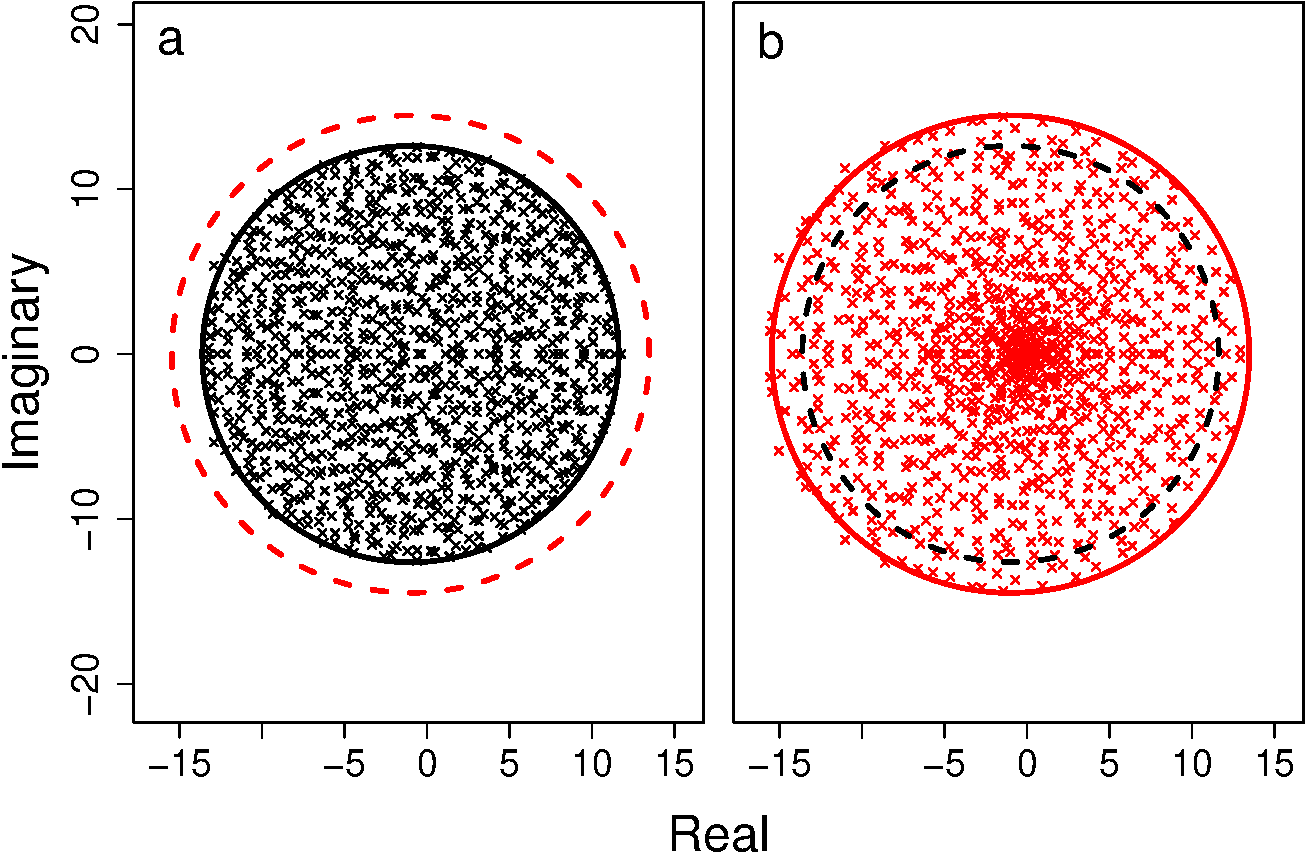
\includegraphics{unnamed-chunk-8-1.pdf}

\hypertarget{IncrS}{\section{\texorpdfstring{Stability across increasing
\(S\)}{Stability across increasing S}}\label{IncrS}}

Figure 3 of the main text reports the number of stable random complex
systems found over 1 million iterations. The data used to make this
figure are read into R below.

\begin{Shaded}
\begin{Highlighting}[]
\NormalTok{dat <-}\StringTok{ }\KeywordTok{read.csv}\NormalTok{(}\DataTypeTok{file =} \StringTok{"sim_results/C_1/random_all.csv"}\NormalTok{);}
\NormalTok{dat <-}\StringTok{ }\NormalTok{dat[,-}\DecValTok{1}\NormalTok{]; }\CommentTok{# Extra row-indicating column removed}
\end{Highlighting}
\end{Shaded}

The table below shows the results for all simulations of random \(M\)
matrices at \(\sigma = 0.4\) and \(C = 1\) given a range of
\(S = \{2, 3, ..., 49, 50\}\). In this table, the \texttt{A0} refers to
matrices where \(\gamma = 1\), while \texttt{A1} refers to matrices
after \(Var(\gamma)\) is added and \(\gamma \sim \mathcal{U}(0, 2)\).
Each row summarises data for a given \(S\) over 1 million randomly
simulated \(M\) (\texttt{A0} and \texttt{A1}). The column
\texttt{A0\_unstable} shows the number of \texttt{A0} matrices that are
unstable, and the column \texttt{A0\_stable} shows the number of
\texttt{A0} matrices that are stable (these two columns sum to 1
million). Similarly, the column \texttt{A1\_unstable} shows the number
of \texttt{A1} matrices that are unstable and \texttt{A1\_stable} shows
the number that are stable. The columns \texttt{A1\_stabilised} and
\texttt{A1\_destabilised} show how many \texttt{A0} matrices were
stabilised or destabilised, respectively, by \(Var(\gamma)\).

\begin{longtable}[]{@{}rrrrrrr@{}}
\toprule
S & A0\_unstable & A0\_stable & A1\_unstable & A1\_stable &
A1\_stabilised & A1\_destabilised\tabularnewline
\midrule
\endhead
2 & 293 & 999707 & 293 & 999707 & 0 & 0\tabularnewline
3 & 3602 & 996398 & 3609 & 996391 & 0 & 7\tabularnewline
4 & 14937 & 985063 & 15008 & 984992 & 0 & 71\tabularnewline
5 & 39289 & 960711 & 39783 & 960217 & 36 & 530\tabularnewline
6 & 78845 & 921155 & 80207 & 919793 & 389 & 1751\tabularnewline
7 & 133764 & 866236 & 136904 & 863096 & 1679 & 4819\tabularnewline
8 & 204112 & 795888 & 208241 & 791759 & 5391 & 9520\tabularnewline
9 & 288041 & 711959 & 291775 & 708225 & 12619 & 16353\tabularnewline
10 & 384024 & 615976 & 384931 & 615069 & 23153 & 24060\tabularnewline
11 & 485975 & 514025 & 481019 & 518981 & 35681 & 30725\tabularnewline
12 & 590453 & 409547 & 577439 & 422561 & 48302 & 35288\tabularnewline
13 & 689643 & 310357 & 669440 & 330560 & 57194 & 36991\tabularnewline
14 & 777496 & 222504 & 751433 & 248567 & 60959 & 34896\tabularnewline
15 & 850159 & 149841 & 821613 & 178387 & 58567 & 30021\tabularnewline
16 & 905057 & 94943 & 877481 & 122519 & 51255 & 23679\tabularnewline
17 & 943192 & 56808 & 919536 & 80464 & 40854 & 17198\tabularnewline
18 & 969018 & 30982 & 949944 & 50056 & 30102 & 11028\tabularnewline
19 & 984301 & 15699 & 970703 & 29297 & 20065 & 6467\tabularnewline
20 & 992601 & 7399 & 983507 & 16493 & 12587 & 3493\tabularnewline
21 & 996765 & 3235 & 991532 & 8468 & 7030 & 1797\tabularnewline
22 & 998693 & 1307 & 995567 & 4433 & 3884 & 758\tabularnewline
23 & 999503 & 497 & 997941 & 2059 & 1883 & 321\tabularnewline
24 & 999861 & 139 & 999059 & 941 & 899 & 97\tabularnewline
25 & 999964 & 36 & 999617 & 383 & 380 & 33\tabularnewline
26 & 999993 & 7 & 999878 & 122 & 121 & 6\tabularnewline
27 & 999995 & 5 & 999946 & 54 & 53 & 4\tabularnewline
28 & 1000000 & 0 & 999975 & 25 & 25 & 0\tabularnewline
29 & 1000000 & 0 & 999997 & 3 & 3 & 0\tabularnewline
30 & 1000000 & 0 & 999999 & 1 & 1 & 0\tabularnewline
31 & 1000000 & 0 & 999999 & 1 & 1 & 0\tabularnewline
32 & 1000000 & 0 & 1000000 & 0 & 0 & 0\tabularnewline
33 & 1000000 & 0 & 1000000 & 0 & 0 & 0\tabularnewline
34 & 1000000 & 0 & 1000000 & 0 & 0 & 0\tabularnewline
35 & 1000000 & 0 & 1000000 & 0 & 0 & 0\tabularnewline
36 & 1000000 & 0 & 1000000 & 0 & 0 & 0\tabularnewline
37 & 1000000 & 0 & 1000000 & 0 & 0 & 0\tabularnewline
38 & 1000000 & 0 & 1000000 & 0 & 0 & 0\tabularnewline
39 & 1000000 & 0 & 1000000 & 0 & 0 & 0\tabularnewline
40 & 1000000 & 0 & 1000000 & 0 & 0 & 0\tabularnewline
41 & 1000000 & 0 & 1000000 & 0 & 0 & 0\tabularnewline
42 & 1000000 & 0 & 1000000 & 0 & 0 & 0\tabularnewline
43 & 1000000 & 0 & 1000000 & 0 & 0 & 0\tabularnewline
44 & 1000000 & 0 & 1000000 & 0 & 0 & 0\tabularnewline
45 & 1000000 & 0 & 1000000 & 0 & 0 & 0\tabularnewline
46 & 1000000 & 0 & 1000000 & 0 & 0 & 0\tabularnewline
47 & 1000000 & 0 & 1000000 & 0 & 0 & 0\tabularnewline
48 & 1000000 & 0 & 1000000 & 0 & 0 & 0\tabularnewline
49 & 1000000 & 0 & 1000000 & 0 & 0 & 0\tabularnewline
50 & 1000000 & 0 & 1000000 & 0 & 0 & 0\tabularnewline
\bottomrule
\end{longtable}

Overall, the ratio of stable \texttt{A1} matrices to stable \texttt{A0}
matrices found is greater than 1 (compare column 5 to column 3), and
this ratio increases with increasing \(S\) (column 1). Hence, more
randomly created complex systems (\(M\)) are generated given variation
in \(\gamma\) than when \(\gamma = 1\). The results underlying this
table were produced with the \texttt{rand\_gen\_var} function below.

\begin{Shaded}
\begin{Highlighting}[]
\NormalTok{rand_gen_var <-}\StringTok{ }\NormalTok{function(max_sp, iters, }\DataTypeTok{int_type =} \DecValTok{0}\NormalTok{, }\DataTypeTok{rmx =} \FloatTok{0.4}\NormalTok{, }\DataTypeTok{C =} \DecValTok{1}\NormalTok{)\{}
    \NormalTok{tot_res <-}\StringTok{ }\OtherTok{NULL}\NormalTok{;}
    \NormalTok{fea_res <-}\StringTok{ }\OtherTok{NULL}\NormalTok{;}
    \NormalTok{for(i in }\DecValTok{2}\NormalTok{:max_sp)\{}
        \NormalTok{iter           <-}\StringTok{ }\NormalTok{iters;}
        \NormalTok{tot_res[[i}\DecValTok{-1}\NormalTok{]] <-}\StringTok{ }\KeywordTok{matrix}\NormalTok{(}\DataTypeTok{data =} \DecValTok{0}\NormalTok{, }\DataTypeTok{nrow =} \NormalTok{iter, }\DataTypeTok{ncol =} \DecValTok{7}\NormalTok{);}
        \NormalTok{fea_res[[i}\DecValTok{-1}\NormalTok{]] <-}\StringTok{ }\KeywordTok{matrix}\NormalTok{(}\DataTypeTok{data =} \DecValTok{0}\NormalTok{, }\DataTypeTok{nrow =} \NormalTok{iter, }\DataTypeTok{ncol =} \DecValTok{7}\NormalTok{);}
        \NormalTok{while(iter >}\StringTok{ }\DecValTok{0}\NormalTok{)\{}
            \NormalTok{r_vec    <-}\StringTok{ }\KeywordTok{rnorm}\NormalTok{(}\DataTypeTok{n =} \NormalTok{i, }\DataTypeTok{mean =} \DecValTok{0}\NormalTok{, }\DataTypeTok{sd =} \NormalTok{rmx);}
            \NormalTok{A0_dat   <-}\StringTok{ }\KeywordTok{rnorm}\NormalTok{(}\DataTypeTok{n =} \NormalTok{i *}\StringTok{ }\NormalTok{i, }\DataTypeTok{mean =} \DecValTok{0}\NormalTok{, }\DataTypeTok{sd =} \FloatTok{0.4}\NormalTok{);}
            \NormalTok{A0       <-}\StringTok{ }\KeywordTok{matrix}\NormalTok{(}\DataTypeTok{data =} \NormalTok{A0_dat, }\DataTypeTok{nrow =} \NormalTok{i, }\DataTypeTok{ncol =} \NormalTok{i);}
            \NormalTok{A0       <-}\StringTok{ }\KeywordTok{species_interactions}\NormalTok{(}\DataTypeTok{mat =} \NormalTok{A0, }\DataTypeTok{type =} \NormalTok{int_type);}
            \NormalTok{C_dat    <-}\StringTok{ }\KeywordTok{rbinom}\NormalTok{(}\DataTypeTok{n =} \NormalTok{i *}\StringTok{ }\NormalTok{i, }\DataTypeTok{size =} \DecValTok{1}\NormalTok{, }\DataTypeTok{prob =} \NormalTok{C);}
            \NormalTok{C_mat    <-}\StringTok{ }\KeywordTok{matrix}\NormalTok{(}\DataTypeTok{data =} \NormalTok{C_dat, }\DataTypeTok{nrow =} \NormalTok{i, }\DataTypeTok{ncol =} \NormalTok{i);}
            \NormalTok{A0       <-}\StringTok{ }\NormalTok{A0 *}\StringTok{ }\NormalTok{C_mat;}
            \KeywordTok{diag}\NormalTok{(A0) <-}\StringTok{ }\NormalTok{-}\DecValTok{1}\NormalTok{;}
            \NormalTok{gam1     <-}\StringTok{ }\KeywordTok{runif}\NormalTok{(}\DataTypeTok{n =} \NormalTok{i, }\DataTypeTok{min =} \DecValTok{0}\NormalTok{, }\DataTypeTok{max =} \DecValTok{2}\NormalTok{);}
            \NormalTok{A1       <-}\StringTok{ }\NormalTok{A0 *}\StringTok{ }\NormalTok{gam1;}
            \NormalTok{A0       <-}\StringTok{ }\NormalTok{A0 *}\StringTok{ }\KeywordTok{mean}\NormalTok{(gam1);}
            \NormalTok{A0_stb   <-}\StringTok{ }\KeywordTok{max}\NormalTok{(}\KeywordTok{Re}\NormalTok{(}\KeywordTok{eigen}\NormalTok{(A0)$values)) <}\StringTok{ }\DecValTok{0}\NormalTok{;}
            \NormalTok{A1_stb   <-}\StringTok{ }\KeywordTok{max}\NormalTok{(}\KeywordTok{Re}\NormalTok{(}\KeywordTok{eigen}\NormalTok{(A1)$values)) <}\StringTok{ }\DecValTok{0}\NormalTok{;}
            \NormalTok{A0_fea   <-}\StringTok{ }\KeywordTok{min}\NormalTok{(-}\DecValTok{1}\NormalTok{*}\KeywordTok{solve}\NormalTok{(A0) %*%}\StringTok{ }\NormalTok{r_vec) >}\StringTok{ }\DecValTok{0}\NormalTok{;}
            \NormalTok{A1_fea   <-}\StringTok{ }\KeywordTok{min}\NormalTok{(-}\DecValTok{1}\NormalTok{*}\KeywordTok{solve}\NormalTok{(A1) %*%}\StringTok{ }\NormalTok{r_vec) >}\StringTok{ }\DecValTok{0}\NormalTok{;}
            \NormalTok{if(A0_stb ==}\StringTok{ }\OtherTok{TRUE}\NormalTok{)\{}
                \NormalTok{tot_res[[i}\DecValTok{-1}\NormalTok{]][iter, }\DecValTok{1}\NormalTok{] <-}\StringTok{ }\DecValTok{1}\NormalTok{;}
            \NormalTok{\}}
            \NormalTok{if(A1_stb ==}\StringTok{ }\OtherTok{TRUE}\NormalTok{)\{}
                \NormalTok{tot_res[[i}\DecValTok{-1}\NormalTok{]][iter, }\DecValTok{2}\NormalTok{] <-}\StringTok{ }\DecValTok{1}\NormalTok{;}
            \NormalTok{\}}
            \NormalTok{if(A0_fea ==}\StringTok{ }\OtherTok{TRUE}\NormalTok{)\{}
                \NormalTok{fea_res[[i}\DecValTok{-1}\NormalTok{]][iter, }\DecValTok{1}\NormalTok{] <-}\StringTok{ }\DecValTok{1}\NormalTok{;}
            \NormalTok{\}}
            \NormalTok{if(A1_fea ==}\StringTok{ }\OtherTok{TRUE}\NormalTok{)\{}
                \NormalTok{fea_res[[i}\DecValTok{-1}\NormalTok{]][iter, }\DecValTok{2}\NormalTok{] <-}\StringTok{ }\DecValTok{1}\NormalTok{;}
            \NormalTok{\}}
            \NormalTok{iter    <-}\StringTok{ }\NormalTok{iter -}\StringTok{ }\DecValTok{1}\NormalTok{;}
        \NormalTok{\}}
        \KeywordTok{print}\NormalTok{(i);}
    \NormalTok{\}}
    \NormalTok{all_res <-}\StringTok{ }\KeywordTok{summarise_randmat}\NormalTok{(}\DataTypeTok{tot_res =} \NormalTok{tot_res, }\DataTypeTok{fea_res =} \NormalTok{fea_res);}
    \KeywordTok{return}\NormalTok{(all_res);}
\NormalTok{\}}
\end{Highlighting}
\end{Shaded}

The above function calls the two functions
\texttt{species\_interactions} and \texttt{summarise\_randmat}, which
are provided below.

\begin{Shaded}
\begin{Highlighting}[]
\NormalTok{species_interactions <-}\StringTok{ }\NormalTok{function(mat, }\DataTypeTok{type =} \DecValTok{0}\NormalTok{)\{}
    \NormalTok{if(type ==}\StringTok{ }\DecValTok{1}\NormalTok{)\{}
        \NormalTok{mat[mat >}\StringTok{ }\DecValTok{0}\NormalTok{] <-}\StringTok{ }\NormalTok{-}\DecValTok{1}\NormalTok{*mat[mat >}\StringTok{ }\DecValTok{0}\NormalTok{];}
    \NormalTok{\}}
    \NormalTok{if(type ==}\StringTok{ }\DecValTok{2}\NormalTok{)\{}
        \NormalTok{mat[mat <}\StringTok{ }\DecValTok{0}\NormalTok{] <-}\StringTok{ }\NormalTok{-}\DecValTok{1}\NormalTok{*mat[mat <}\StringTok{ }\DecValTok{0}\NormalTok{];}
    \NormalTok{\}}
    \NormalTok{if(type ==}\StringTok{ }\DecValTok{3}\NormalTok{)\{}
        \NormalTok{for(i in }\DecValTok{1}\NormalTok{:}\KeywordTok{dim}\NormalTok{(mat)[}\DecValTok{1}\NormalTok{])\{}
            \NormalTok{for(j in }\DecValTok{1}\NormalTok{:}\KeywordTok{dim}\NormalTok{(mat)[}\DecValTok{2}\NormalTok{])\{}
                \NormalTok{if(mat[i, j] *}\StringTok{ }\NormalTok{mat[j, i] >}\StringTok{ }\DecValTok{0}\NormalTok{)\{}
                    \NormalTok{mat[j, i] <-}\StringTok{ }\NormalTok{-}\DecValTok{1} \NormalTok{*}\StringTok{ }\NormalTok{mat[j, i];}
                \NormalTok{\}}
            \NormalTok{\}}
        \NormalTok{\}}
    \NormalTok{\}}
    \KeywordTok{return}\NormalTok{(mat);}
\NormalTok{\}}

\NormalTok{summarise_randmat <-}\StringTok{ }\NormalTok{function(tot_res, fea_res)\{}
    \NormalTok{sims    <-}\StringTok{ }\KeywordTok{length}\NormalTok{(tot_res);}
    \NormalTok{all_res <-}\StringTok{ }\KeywordTok{matrix}\NormalTok{(}\DataTypeTok{data =} \DecValTok{0}\NormalTok{, }\DataTypeTok{nrow =} \NormalTok{sims, }\DataTypeTok{ncol =} \DecValTok{13}\NormalTok{);}
    \NormalTok{for(i in }\DecValTok{1}\NormalTok{:sims)\{}
        \NormalTok{all_res[i, }\DecValTok{1}\NormalTok{]  <-}\StringTok{ }\NormalTok{i +}\StringTok{ }\DecValTok{1}\NormalTok{;}
        \CommentTok{# Stable and unstable}
        \NormalTok{all_res[i, }\DecValTok{2}\NormalTok{]  <-}\StringTok{ }\KeywordTok{sum}\NormalTok{(tot_res[[i]][,}\DecValTok{1}\NormalTok{] ==}\StringTok{ }\OtherTok{FALSE}\NormalTok{);}
        \NormalTok{all_res[i, }\DecValTok{3}\NormalTok{]  <-}\StringTok{ }\KeywordTok{sum}\NormalTok{(tot_res[[i]][,}\DecValTok{1}\NormalTok{] ==}\StringTok{ }\OtherTok{TRUE}\NormalTok{);}
        \NormalTok{all_res[i, }\DecValTok{4}\NormalTok{]  <-}\StringTok{ }\KeywordTok{sum}\NormalTok{(tot_res[[i]][,}\DecValTok{2}\NormalTok{] ==}\StringTok{ }\OtherTok{FALSE}\NormalTok{);}
        \NormalTok{all_res[i, }\DecValTok{5}\NormalTok{]  <-}\StringTok{ }\KeywordTok{sum}\NormalTok{(tot_res[[i]][,}\DecValTok{2}\NormalTok{] ==}\StringTok{ }\OtherTok{TRUE}\NormalTok{);}
        \CommentTok{# Stabilised and destabilised}
        \NormalTok{all_res[i, }\DecValTok{6}\NormalTok{] <-}\StringTok{ }\KeywordTok{sum}\NormalTok{(tot_res[[i]][,}\DecValTok{1}\NormalTok{] ==}\StringTok{ }\OtherTok{FALSE} \NormalTok{&}\StringTok{ }
\StringTok{                                  }\NormalTok{tot_res[[i]][,}\DecValTok{2}\NormalTok{] ==}\StringTok{ }\OtherTok{TRUE}\NormalTok{);}
        \NormalTok{all_res[i, }\DecValTok{7}\NormalTok{] <-}\StringTok{ }\KeywordTok{sum}\NormalTok{(tot_res[[i]][,}\DecValTok{1}\NormalTok{] ==}\StringTok{ }\OtherTok{TRUE} \NormalTok{&}\StringTok{ }
\StringTok{                                  }\NormalTok{tot_res[[i]][,}\DecValTok{2}\NormalTok{] ==}\StringTok{ }\OtherTok{FALSE}\NormalTok{);}
        \CommentTok{# Feasible and infeasible}
        \NormalTok{all_res[i, }\DecValTok{8}\NormalTok{]  <-}\StringTok{ }\KeywordTok{sum}\NormalTok{(fea_res[[i]][,}\DecValTok{1}\NormalTok{] ==}\StringTok{ }\OtherTok{FALSE}\NormalTok{);}
        \NormalTok{all_res[i, }\DecValTok{9}\NormalTok{]  <-}\StringTok{ }\KeywordTok{sum}\NormalTok{(fea_res[[i]][,}\DecValTok{1}\NormalTok{] ==}\StringTok{ }\OtherTok{TRUE}\NormalTok{);}
        \NormalTok{all_res[i, }\DecValTok{10}\NormalTok{]  <-}\StringTok{ }\KeywordTok{sum}\NormalTok{(fea_res[[i]][,}\DecValTok{2}\NormalTok{] ==}\StringTok{ }\OtherTok{FALSE}\NormalTok{);}
        \NormalTok{all_res[i, }\DecValTok{11}\NormalTok{]  <-}\StringTok{ }\KeywordTok{sum}\NormalTok{(fea_res[[i]][,}\DecValTok{2}\NormalTok{] ==}\StringTok{ }\OtherTok{TRUE}\NormalTok{);}
        \CommentTok{# Feased and defeased}
        \NormalTok{all_res[i, }\DecValTok{12}\NormalTok{] <-}\StringTok{ }\KeywordTok{sum}\NormalTok{(fea_res[[i]][,}\DecValTok{1}\NormalTok{] ==}\StringTok{ }\OtherTok{FALSE} \NormalTok{&}\StringTok{ }
\StringTok{                                  }\NormalTok{fea_res[[i]][,}\DecValTok{2}\NormalTok{] ==}\StringTok{ }\OtherTok{TRUE}\NormalTok{);}
        \NormalTok{all_res[i, }\DecValTok{13}\NormalTok{] <-}\StringTok{ }\KeywordTok{sum}\NormalTok{(fea_res[[i]][,}\DecValTok{1}\NormalTok{] ==}\StringTok{ }\OtherTok{TRUE} \NormalTok{&}\StringTok{ }
\StringTok{                                  }\NormalTok{fea_res[[i]][,}\DecValTok{2}\NormalTok{] ==}\StringTok{ }\OtherTok{FALSE}\NormalTok{);}
    \NormalTok{\}}
    \NormalTok{cnames <-}\StringTok{ }\KeywordTok{c}\NormalTok{(}\StringTok{"N"}\NormalTok{, }\StringTok{"A0_unstable"}\NormalTok{, }\StringTok{"A0_stable"}\NormalTok{, }\StringTok{"A1_unstable"}\NormalTok{, }\StringTok{"A1_stable"}\NormalTok{, }
                \StringTok{"A1_stabilised"}\NormalTok{, }\StringTok{"A1_destabilised"}\NormalTok{, }\StringTok{"A0_infeasible"}\NormalTok{, }
                \StringTok{"A0_feasible"}\NormalTok{, }\StringTok{"A1_infeasible"}\NormalTok{, }\StringTok{"A1_feasible"}\NormalTok{, }
                \StringTok{"A1_made_feasible"}\NormalTok{, }\StringTok{"A1_made_infeasible"}\NormalTok{);}
    \KeywordTok{colnames}\NormalTok{(all_res) <-}\StringTok{ }\NormalTok{cnames;}
    \KeywordTok{return}\NormalTok{(all_res);}
\NormalTok{\}}
\end{Highlighting}
\end{Shaded}

Note that feasibility results were ommited for the table above, but are
\protect\hyperlink{Feasibility}{reported below}.

\hypertarget{ecological}{\section{Stability of ecological
networks}\label{ecological}}

While the foundational work of
May\textsuperscript{\protect\hyperlink{ref-May1972}{1}} applies broadly
to complex networks, much attention has been given specifically to
ecological networks of interacting species. In these networks, the
matrix \(M\) is interpreted as a community matrix and each row and
column is interpreted as a single species. The effect that the density
of any species \(i\) has on the population dynamics of species \(j\) is
found in \(M_{ij}\), meaning that \(M\) holds the effects of pair-wise
interactions between \(S\)
species\textsuperscript{\protect\hyperlink{ref-Allesina2012}{2}--\protect\hyperlink{ref-Tang2014b}{4}}.
While May's original
work\textsuperscript{\protect\hyperlink{ref-May1972}{1}} considered only
randomly assembled communities, recent work has specifically looked at
more restricted ecological communities including competitive networks
(all off-diagonal elements of \(M\) are negative), mutualist networks
(all off-diagonal elements of \(M\) are positive), and predator-prey
networks (for any pair of \(i\) and \(j\), the effect of \(i\) on \(j\)
is negative and \(j\) on \(i\) is positive, or vice
versa)\textsuperscript{\protect\hyperlink{ref-Allesina2012}{2}--\protect\hyperlink{ref-Allesina2011}{5}}.
In general, competitor and mutualist networks tend to be unstable, while
predator-prey networks tend to be highly stabilising.

I investigated competitor, mutualist, and predator-prey networks
following Allesina et
al.\textsuperscript{\protect\hyperlink{ref-Allesina2012}{2}}. To create
these networks, I first generated a random matrix \(M\), then changed
the elements of \(M\) accordingly. If \(M\) was a competitive network,
then the sign of any positive off-diagonal elements was reversed to be
negative. If \(M\) was a mutualist network, then the sign of any
positive off-diagonal elements was reversed to be positive. And if \(M\)
was a predator-prey network, then all \(i\) and \(j\) pairs of elements
were checked; any pairs of the same sign were changed so that one was
negative and the other was positive. The \texttt{species\_interaction}
function used to do this is below.

\begin{Shaded}
\begin{Highlighting}[]
\NormalTok{species_interactions <-}\StringTok{ }\NormalTok{function(mat, }\DataTypeTok{type =} \DecValTok{0}\NormalTok{)\{}
    \NormalTok{if(type ==}\StringTok{ }\DecValTok{1}\NormalTok{)\{}
        \NormalTok{mat[mat >}\StringTok{ }\DecValTok{0}\NormalTok{] <-}\StringTok{ }\NormalTok{-}\DecValTok{1}\NormalTok{*mat[mat >}\StringTok{ }\DecValTok{0}\NormalTok{];}
    \NormalTok{\}}
    \NormalTok{if(type ==}\StringTok{ }\DecValTok{2}\NormalTok{)\{}
        \NormalTok{mat[mat <}\StringTok{ }\DecValTok{0}\NormalTok{] <-}\StringTok{ }\NormalTok{-}\DecValTok{1}\NormalTok{*mat[mat <}\StringTok{ }\DecValTok{0}\NormalTok{];}
    \NormalTok{\}}
    \NormalTok{if(type ==}\StringTok{ }\DecValTok{3}\NormalTok{)\{}
        \NormalTok{for(i in }\DecValTok{1}\NormalTok{:}\KeywordTok{dim}\NormalTok{(mat)[}\DecValTok{1}\NormalTok{])\{}
            \NormalTok{for(j in }\DecValTok{1}\NormalTok{:}\KeywordTok{dim}\NormalTok{(mat)[}\DecValTok{2}\NormalTok{])\{}
                \NormalTok{if(mat[i, j] *}\StringTok{ }\NormalTok{mat[j, i] >}\StringTok{ }\DecValTok{0}\NormalTok{)\{}
                    \NormalTok{mat[j, i] <-}\StringTok{ }\NormalTok{-}\DecValTok{1} \NormalTok{*}\StringTok{ }\NormalTok{mat[j, i];}
                \NormalTok{\}}
            \NormalTok{\}}
        \NormalTok{\}}
    \NormalTok{\}}
    \KeywordTok{return}\NormalTok{(mat);}
\NormalTok{\} }\CommentTok{# Note: -1 values are added in the diagonal later}
\end{Highlighting}
\end{Shaded}

This function was applied to all created matrices \(M\), then the number
of stable \(M\) matrices was estimated \protect\hyperlink{IncrS}{exactly
as it was} in the main text for random matrices for values of \(S\) from
2 to 50 (100 in the case of the relatively more stable predator-prey
interactions), except that only 100000 random \(M\) were generated
instead of 1 million. This produced the data set below.

\begin{Shaded}
\begin{Highlighting}[]
\NormalTok{cdat <-}\StringTok{ }\KeywordTok{read.csv}\NormalTok{(}\DataTypeTok{file =} \StringTok{"sim_results/ecology/competition_C_1.csv"}\NormalTok{);}
\NormalTok{mdat <-}\StringTok{ }\KeywordTok{read.csv}\NormalTok{(}\DataTypeTok{file =} \StringTok{"sim_results/ecology/mutualism_C_1.csv"}\NormalTok{);}
\NormalTok{pdat <-}\StringTok{ }\KeywordTok{read.csv}\NormalTok{(}\DataTypeTok{file =} \StringTok{"sim_results/ecology/pred-prey_C_1.csv"}\NormalTok{);}
\end{Highlighting}
\end{Shaded}

The following tables for restricted ecological communities can therefore
be compared with the random \(M\) \protect\hyperlink{IncrS}{results
above} (but note that counts from systems with comparable probabilities
of stability will be an order of magnitude lower in the tables below due
to the smaller number of \(M\) matrices generated). As with the
\protect\hyperlink{IncrS}{results above}, in the tables below,
\texttt{A0} refers to matrices when \(\gamma = 1\) and \texttt{A1}
refers to matrices after \(Var(\gamma)\) is added. The column
\texttt{A0\_unstable} shows the number of \texttt{A0} matrices that are
unstable, and the column \texttt{A0\_stable} shows the number of
\texttt{A0} matrices that are stable (these two columns sum to 100000).
Similarly, the column \texttt{A1\_unstable} shows the number of
\texttt{A1} matrices that are unstable and \texttt{A1\_stable} shows the
number that are stable. The columns \texttt{A1\_stabilised} and
\texttt{A1\_destabilised} show how many \texttt{A0} matrices were
stabilised or destabilised, respectively, by \(Var(\gamma)\).

\textbf{Competition}

Results for competitor interaction networks are shown below

\begin{longtable}[]{@{}llllll@{}}
\toprule
N & A0\_unstable & A0\_stable & A1\_unstable & A1\_stable &
A1\_stabilised\tabularnewline
\midrule
\endhead
2 & 48 & 99952 & 48 & 99952 & 0\tabularnewline
3 & 229 & 99771 & 231 & 99769 & 0\tabularnewline
4 & 701 & 99299 & 704 & 99296 & 0\tabularnewline
5 & 1579 & 98421 & 1587 & 98413 & 0\tabularnewline
6 & 3218 & 96782 & 3253 & 96747 & 6\tabularnewline
7 & 5519 & 94481 & 5619 & 94381 & 23\tabularnewline
8 & 9062 & 90938 & 9237 & 90763 & 77\tabularnewline
9 & 13436 & 86564 & 13729 & 86271 & 230\tabularnewline
10 & 18911 & 81089 & 19303 & 80697 & 505\tabularnewline
11 & 25594 & 74406 & 25961 & 74039 & 1011\tabularnewline
12 & 33207 & 66793 & 33382 & 66618 & 1724\tabularnewline
13 & 41160 & 58840 & 41089 & 58911 & 2655\tabularnewline
14 & 50575 & 49425 & 49894 & 50106 & 3777\tabularnewline
15 & 59250 & 40750 & 57892 & 42108 & 4824\tabularnewline
16 & 67811 & 32189 & 65740 & 34260 & 5634\tabularnewline
17 & 75483 & 24517 & 73056 & 26944 & 5943\tabularnewline
18 & 82551 & 17449 & 79878 & 20122 & 5780\tabularnewline
19 & 88030 & 11970 & 85204 & 14796 & 5417\tabularnewline
20 & 92254 & 7746 & 89766 & 10234 & 4544\tabularnewline
21 & 95233 & 4767 & 93002 & 6998 & 3695\tabularnewline
22 & 97317 & 2683 & 95451 & 4549 & 2803\tabularnewline
23 & 98508 & 1492 & 97122 & 2878 & 1991\tabularnewline
24 & 99240 & 760 & 98407 & 1593 & 1216\tabularnewline
25 & 99669 & 331 & 99082 & 918 & 739\tabularnewline
26 & 99871 & 129 & 99490 & 510 & 452\tabularnewline
27 & 99938 & 62 & 99732 & 268 & 240\tabularnewline
28 & 99985 & 15 & 99888 & 112 & 108\tabularnewline
29 & 99990 & 10 & 99951 & 49 & 46\tabularnewline
30 & 100000 & 0 & 99981 & 19 & 19\tabularnewline
31 & 100000 & 0 & 99993 & 7 & 7\tabularnewline
32 & 100000 & 0 & 99996 & 4 & 4\tabularnewline
33 & 100000 & 0 & 99998 & 2 & 2\tabularnewline
34 & 100000 & 0 & 100000 & 0 & 0\tabularnewline
\ldots{} & \ldots{} & \ldots{} & \ldots{} & \ldots{} & \ldots{} \tabularnewline
50 & 100000 & 0 & 100000 & 0 & 0\tabularnewline
\bottomrule
\end{longtable}

\textbf{Mutualism}

Results for mutualist interaction networks are shown below

\begin{longtable}[]{@{}llllll@{}}
\toprule
N & A0\_unstable & A0\_stable & A1\_unstable & A1\_stable &
A1\_stabilised\tabularnewline
\midrule
\endhead
2 & 56 & 99944 & 56 & 99944 & 0\tabularnewline
3 & 3301 & 96699 & 3301 & 96699 & 0\tabularnewline
4 & 34446 & 65554 & 34446 & 65554 & 0\tabularnewline
5 & 86520 & 13480 & 86520 & 13480 & 0\tabularnewline
6 & 99683 & 317 & 99683 & 317 & 0\tabularnewline
7 & 99998 & 2 & 99998 & 2 & 0\tabularnewline
8 & 100000 & 0 & 100000 & 0 & 0\tabularnewline
9 & 100000 & 0 & 100000 & 0 & 0\tabularnewline
10 & 100000 & 0 & 100000 & 0 & 0\tabularnewline
11 & 100000 & 0 & 100000 & 0 & 0\tabularnewline
12 & 100000 & 0 & 100000 & 0 & 0\tabularnewline
\ldots{} & \ldots{} & \ldots{} & \ldots{} & \ldots{} & \ldots{} \tabularnewline
50 & 100000 & 0 & 100000 & 0 & 0\tabularnewline
\bottomrule
\end{longtable}

\textbf{Predator-prey}

Results for predator-prey interaction networks are shown below

\begin{longtable}[]{@{}rrrrrr@{}}
\toprule
N & A0\_unstable & A0\_stable & A1\_unstable & A1\_stable &
A1\_stabilised\tabularnewline
\midrule
\endhead
2 & 0 & 100000 & 0 & 100000 & 0\tabularnewline
3 & 0 & 100000 & 0 & 100000 & 0\tabularnewline
4 & 0 & 100000 & 0 & 100000 & 0\tabularnewline
5 & 1 & 99999 & 1 & 99999 & 0\tabularnewline
6 & 4 & 99996 & 4 & 99996 & 0\tabularnewline
7 & 2 & 99998 & 2 & 99998 & 0\tabularnewline
8 & 5 & 99995 & 5 & 99995 & 0\tabularnewline
9 & 20 & 99980 & 21 & 99979 & 0\tabularnewline
10 & 20 & 99980 & 22 & 99978 & 0\tabularnewline
11 & 38 & 99962 & 39 & 99961 & 0\tabularnewline
12 & 64 & 99936 & 66 & 99934 & 0\tabularnewline
13 & 87 & 99913 & 91 & 99909 & 0\tabularnewline
14 & 157 & 99843 & 159 & 99841 & 0\tabularnewline
15 & 215 & 99785 & 227 & 99773 & 0\tabularnewline
16 & 293 & 99707 & 310 & 99690 & 0\tabularnewline
17 & 383 & 99617 & 408 & 99592 & 0\tabularnewline
18 & 443 & 99557 & 473 & 99527 & 3\tabularnewline
19 & 642 & 99358 & 675 & 99325 & 4\tabularnewline
20 & 836 & 99164 & 887 & 99113 & 7\tabularnewline
21 & 1006 & 98994 & 1058 & 98942 & 10\tabularnewline
22 & 1153 & 98847 & 1228 & 98772 & 20\tabularnewline
23 & 1501 & 98499 & 1593 & 98407 & 30\tabularnewline
24 & 1841 & 98159 & 1996 & 98004 & 40\tabularnewline
25 & 2146 & 97854 & 2316 & 97684 & 58\tabularnewline
26 & 2643 & 97357 & 2809 & 97191 & 119\tabularnewline
27 & 3034 & 96966 & 3258 & 96742 & 158\tabularnewline
28 & 3690 & 96310 & 3928 & 96072 & 201\tabularnewline
29 & 4257 & 95743 & 4532 & 95468 & 290\tabularnewline
30 & 4964 & 95036 & 5221 & 94779 & 424\tabularnewline
31 & 5627 & 94373 & 5978 & 94022 & 452\tabularnewline
32 & 6543 & 93457 & 6891 & 93109 & 666\tabularnewline
33 & 7425 & 92575 & 7777 & 92223 & 818\tabularnewline
34 & 8540 & 91460 & 8841 & 91159 & 1071\tabularnewline
35 & 9526 & 90474 & 9842 & 90158 & 1337\tabularnewline
36 & 10617 & 89383 & 10891 & 89109 & 1624\tabularnewline
37 & 12344 & 87656 & 12508 & 87492 & 2021\tabularnewline
38 & 13675 & 86325 & 13877 & 86123 & 2442\tabularnewline
39 & 15264 & 84736 & 15349 & 84651 & 2870\tabularnewline
40 & 17026 & 82974 & 17053 & 82947 & 3363\tabularnewline
41 & 18768 & 81232 & 18614 & 81386 & 3905\tabularnewline
42 & 20791 & 79209 & 20470 & 79530 & 4579\tabularnewline
43 & 23150 & 76850 & 22754 & 77246 & 5217\tabularnewline
44 & 25449 & 74551 & 24184 & 75816 & 6285\tabularnewline
45 & 27702 & 72298 & 26464 & 73536 & 6754\tabularnewline
46 & 30525 & 69475 & 28966 & 71034 & 7646\tabularnewline
47 & 32832 & 67168 & 31125 & 68875 & 8487\tabularnewline
48 & 36152 & 63848 & 33865 & 66135 & 9479\tabularnewline
49 & 38714 & 61286 & 36242 & 63758 & 10125\tabularnewline
50 & 41628 & 58372 & 38508 & 61492 & 11036\tabularnewline
51 & 44483 & 55517 & 41023 & 58977 & 11704\tabularnewline
52 & 48134 & 51866 & 44287 & 55713 & 12573\tabularnewline
53 & 51138 & 48862 & 46721 & 53279 & 13223\tabularnewline
54 & 54261 & 45739 & 49559 & 50441 & 13757\tabularnewline
55 & 57647 & 42353 & 52403 & 47597 & 14324\tabularnewline
56 & 60630 & 39370 & 55293 & 44707 & 14669\tabularnewline
57 & 63647 & 36353 & 57787 & 42213 & 15103\tabularnewline
58 & 66961 & 33039 & 60439 & 39561 & 15450\tabularnewline
59 & 69968 & 30032 & 63708 & 36292 & 15246\tabularnewline
60 & 72838 & 27162 & 66270 & 33730 & 15177\tabularnewline
61 & 75609 & 24391 & 68873 & 31127 & 15006\tabularnewline
62 & 77999 & 22001 & 71318 & 28682 & 14538\tabularnewline
63 & 80616 & 19384 & 73517 & 26483 & 14510\tabularnewline
64 & 83089 & 16911 & 76209 & 23791 & 13784\tabularnewline
65 & 85150 & 14850 & 78086 & 21914 & 13412\tabularnewline
66 & 86908 & 13092 & 80437 & 19563 & 12477\tabularnewline
67 & 88671 & 11329 & 82379 & 17621 & 11718\tabularnewline
68 & 90537 & 9463 & 84483 & 15517 & 10878\tabularnewline
69 & 91969 & 8031 & 86233 & 13767 & 10033\tabularnewline
70 & 93181 & 6819 & 87914 & 12086 & 9070\tabularnewline
71 & 94330 & 5670 & 89200 & 10800 & 8401\tabularnewline
72 & 95324 & 4676 & 90833 & 9167 & 7359\tabularnewline
73 & 96143 & 3857 & 91805 & 8195 & 6726\tabularnewline
74 & 96959 & 3041 & 93065 & 6935 & 5900\tabularnewline
75 & 97543 & 2457 & 93987 & 6013 & 5222\tabularnewline
76 & 97969 & 2031 & 94900 & 5100 & 4481\tabularnewline
77 & 98497 & 1503 & 95756 & 4244 & 3809\tabularnewline
78 & 98744 & 1256 & 96442 & 3558 & 3269\tabularnewline
79 & 99045 & 955 & 96942 & 3058 & 2837\tabularnewline
80 & 99276 & 724 & 97528 & 2472 & 2329\tabularnewline
81 & 99481 & 519 & 97996 & 2004 & 1894\tabularnewline
82 & 99556 & 444 & 98321 & 1679 & 1597\tabularnewline
83 & 99691 & 309 & 98722 & 1278 & 1227\tabularnewline
84 & 99752 & 248 & 98943 & 1057 & 1015\tabularnewline
85 & 99833 & 167 & 99144 & 856 & 837\tabularnewline
86 & 99895 & 105 & 99346 & 654 & 642\tabularnewline
87 & 99925 & 75 & 99461 & 539 & 530\tabularnewline
88 & 99945 & 55 & 99566 & 434 & 428\tabularnewline
89 & 99976 & 24 & 99675 & 325 & 324\tabularnewline
90 & 99977 & 23 & 99756 & 244 & 243\tabularnewline
91 & 99982 & 18 & 99839 & 161 & 155\tabularnewline
92 & 99988 & 12 & 99865 & 135 & 135\tabularnewline
93 & 99994 & 6 & 99885 & 115 & 115\tabularnewline
94 & 99993 & 7 & 99911 & 89 & 88\tabularnewline
95 & 99998 & 2 & 99953 & 47 & 47\tabularnewline
96 & 99999 & 1 & 99965 & 35 & 35\tabularnewline
97 & 99999 & 1 & 99979 & 21 & 21\tabularnewline
98 & 100000 & 0 & 99973 & 27 & 27\tabularnewline
99 & 100000 & 0 & 99984 & 16 & 16\tabularnewline
100 & 100000 & 0 & 99989 & 11 & 11\tabularnewline
\bottomrule
\end{longtable}

Overall, as
expected\textsuperscript{\protect\hyperlink{ref-Allesina2012}{2}},
predator-prey communities are relatively stable while mutualist
communties are highly unstable. But interestingly, while \(Var(\gamma)\)
stabilises predator-prey and competitor communities, it does not
stabilise mutualist communities. This is unsurprising because purely
mutualist communities are characterised by a very
positive\textsuperscript{\protect\hyperlink{ref-Allesina2012}{2}}
leading \(\Re(\lambda)\), and it is highly unlikely that \(Var(\gamma)\)
alone will shift all real parts of eigenvalues to negative values.

\hypertarget{connectance}{\section{Different connectance (C)
values}\label{connectance}}

In the main text, for simplicity, I assumed connectance values of
\(C = 1\), meaning that all off-diagonal elements of a matrix \(M\) were
potentially nonzero and sampled from a normal distribution
\(\mathcal{N}(0, \sigma^{2})\) where \(\sigma = 0.4\). Here I present
four tables showing the number of stable communities given
\(C = \{0.3, 0. 5, 0.7, 0.9 \}\). In all cases, uniform variation in
component response time (\(\gamma \sim \mathcal{U}(0, 2)\)) led to a
higher number of stable communities than when \(\gamma\) did not vary
(\(\gamma = 1\)). In contrast to the main text, 100000 rather than 1
million \(M\) were simulated. As with the results on
\protect\hyperlink{IncrS}{stability with increasing \(S\)} shown above,
in the tables below \texttt{A0} refers to matrices when \(\gamma = 1\),
and \texttt{A1} refers to matrices after \(Var(\gamma)\) is added. The
column \texttt{A0\_unstable} shows the number of \texttt{A0} matrices
that are unstable, and the column \texttt{A0\_stable} shows the number
of \texttt{A0} matrices that are stable (these two columns sum to
100000). Similarly, the column \texttt{A1\_unstable} shows the number of
\texttt{A1} matrices that are unstable and \texttt{A1\_stable} shows the
number that are stable. The columns \texttt{A1\_stabilised} and
\texttt{A1\_destabilised} show how many \texttt{A0} matrices were
stabilised or destabilised, respectively, by \(Var(\gamma)\).

All data reported below for various values of \(C\) are accessible using
the below.

\begin{Shaded}
\begin{Highlighting}[]
\NormalTok{C3dat <-}\StringTok{ }\KeywordTok{read.csv}\NormalTok{(}\DataTypeTok{file =} \StringTok{"sim_results/C_other/rand_c-0pt3.csv"}\NormalTok{);}
\NormalTok{C5dat <-}\StringTok{ }\KeywordTok{read.csv}\NormalTok{(}\DataTypeTok{file =} \StringTok{"sim_results/C_other/rand_c-0pt5.csv"}\NormalTok{);}
\NormalTok{C7dat <-}\StringTok{ }\KeywordTok{read.csv}\NormalTok{(}\DataTypeTok{file =} \StringTok{"sim_results/C_other/rand_c-0pt7.csv"}\NormalTok{);}
\NormalTok{C9dat <-}\StringTok{ }\KeywordTok{read.csv}\NormalTok{(}\DataTypeTok{file =} \StringTok{"sim_results/C_other/rand_c-0pt9.csv"}\NormalTok{);}
\end{Highlighting}
\end{Shaded}

These objects \texttt{C3dat}, \texttt{C5dat}, \texttt{C7dat}, and
\texttt{C9dat} include the results for \(C = 0.3\), \(C = 0.5\),
\(C = 0.7\), and \(C = 0.9\), respectively.

\textbf{Connectance \(C = 0.3\)}

\begin{longtable}[]{@{}lllllll@{}}
\toprule
N & A0\_unstable & A0\_stable & A1\_unstable & A1\_stable &
A1\_stabilised & A1\_destabilised\tabularnewline
\midrule
\endhead
2 & 5 & 99995 & 5 & 99995 & 0 & 0\tabularnewline
3 & 6 & 99994 & 6 & 99994 & 0 & 0\tabularnewline
4 & 24 & 99976 & 24 & 99976 & 0 & 0\tabularnewline
5 & 59 & 99941 & 59 & 99941 & 0 & 0\tabularnewline
6 & 98 & 99902 & 98 & 99902 & 0 & 0\tabularnewline
7 & 160 & 99840 & 161 & 99839 & 0 & 1\tabularnewline
8 & 290 & 99710 & 293 & 99707 & 0 & 3\tabularnewline
9 & 430 & 99570 & 434 & 99566 & 0 & 4\tabularnewline
10 & 648 & 99352 & 653 & 99347 & 1 & 6\tabularnewline
11 & 946 & 99054 & 957 & 99043 & 0 & 11\tabularnewline
12 & 1392 & 98608 & 1415 & 98585 & 4 & 27\tabularnewline
13 & 2032 & 97968 & 2065 & 97935 & 5 & 38\tabularnewline
14 & 2627 & 97373 & 2688 & 97312 & 10 & 71\tabularnewline
15 & 3588 & 96412 & 3647 & 96353 & 35 & 94\tabularnewline
16 & 5019 & 94981 & 5124 & 94876 & 51 & 156\tabularnewline
17 & 6512 & 93488 & 6673 & 93327 & 79 & 240\tabularnewline
18 & 8444 & 91556 & 8600 & 91400 & 165 & 321\tabularnewline
19 & 10416 & 89584 & 10667 & 89333 & 244 & 495\tabularnewline
20 & 13254 & 86746 & 13477 & 86523 & 425 & 648\tabularnewline
21 & 16248 & 83752 & 16481 & 83519 & 642 & 875\tabularnewline
22 & 19497 & 80503 & 19719 & 80281 & 929 & 1151\tabularnewline
23 & 23654 & 76346 & 23776 & 76224 & 1368 & 1490\tabularnewline
24 & 28485 & 71515 & 28389 & 71611 & 1914 & 1818\tabularnewline
25 & 32774 & 67226 & 32483 & 67517 & 2428 & 2137\tabularnewline
26 & 38126 & 61874 & 37411 & 62589 & 3221 & 2506\tabularnewline
27 & 43435 & 56565 & 42418 & 57582 & 3828 & 2811\tabularnewline
28 & 49333 & 50667 & 47840 & 52160 & 4565 & 3072\tabularnewline
29 & 55389 & 44611 & 53381 & 46619 & 5329 & 3321\tabularnewline
30 & 60826 & 39174 & 58388 & 41612 & 5918 & 3480\tabularnewline
31 & 66820 & 33180 & 64043 & 35957 & 6345 & 3568\tabularnewline
32 & 72190 & 27810 & 69036 & 30964 & 6685 & 3531\tabularnewline
33 & 77053 & 22947 & 73587 & 26413 & 6826 & 3360\tabularnewline
34 & 81816 & 18184 & 78157 & 21843 & 6673 & 3014\tabularnewline
35 & 85651 & 14349 & 82041 & 17959 & 6383 & 2773\tabularnewline
36 & 88985 & 11015 & 85657 & 14343 & 5721 & 2393\tabularnewline
37 & 92072 & 7928 & 88805 & 11195 & 5180 & 1913\tabularnewline
38 & 94329 & 5671 & 91444 & 8556 & 4451 & 1566\tabularnewline
39 & 95912 & 4088 & 93295 & 6705 & 3804 & 1187\tabularnewline
40 & 97232 & 2768 & 95201 & 4799 & 2967 & 936\tabularnewline
41 & 98179 & 1821 & 96506 & 3494 & 2356 & 683\tabularnewline
42 & 98826 & 1174 & 97489 & 2511 & 1786 & 449\tabularnewline
43 & 99275 & 725 & 98312 & 1688 & 1251 & 288\tabularnewline
44 & 99583 & 417 & 98872 & 1128 & 903 & 192\tabularnewline
45 & 99776 & 224 & 99339 & 661 & 576 & 139\tabularnewline
46 & 99865 & 135 & 99518 & 482 & 413 & 66\tabularnewline
47 & 99938 & 62 & 99744 & 256 & 226 & 32\tabularnewline
48 & 99956 & 44 & 99824 & 176 & 151 & 19\tabularnewline
49 & 99980 & 20 & 99914 & 86 & 85 & 19\tabularnewline
50 & 99993 & 7 & 99950 & 50 & 46 & 3\tabularnewline
51 & 99998 & 2 & 99971 & 29 & 28 & 1\tabularnewline
52 & 99998 & 2 & 99986 & 14 & 14 & 2\tabularnewline
53 & 99999 & 1 & 99992 & 8 & 7 & 0\tabularnewline
54 & 100000 & 0 & 99997 & 3 & 3 & 0\tabularnewline
55 & 100000 & 0 & 99999 & 1 & 1 & 0\tabularnewline
56 & 100000 & 0 & 99998 & 2 & 2 & 0\tabularnewline
57 & 100000 & 0 & 99999 & 1 & 1 & 0\tabularnewline
58 & 100000 & 0 & 100000 & 0 & 0 & 0\tabularnewline
\ldots{} & \ldots{} & \ldots{} & \ldots{} & \ldots{} & \ldots{} &
\ldots{}\tabularnewline
100 & 100000 & 0 & 100000 & 0 & 0 & 0\tabularnewline
\bottomrule
\end{longtable}

\textbf{Connectance \(C = 0.5\)}

\begin{longtable}[]{@{}lllllll@{}}
\toprule
N & A0\_unstable & A0\_stable & A1\_unstable & A1\_stable &
A1\_stabilised & A1\_destabilised\tabularnewline
\midrule
\endhead
2 & 7 & 99993 & 7 & 99993 & 0 & 0\tabularnewline
3 & 32 & 99968 & 32 & 99968 & 0 & 0\tabularnewline
4 & 122 & 99878 & 122 & 99878 & 0 & 0\tabularnewline
5 & 320 & 99680 & 321 & 99679 & 0 & 1\tabularnewline
6 & 667 & 99333 & 673 & 99327 & 0 & 6\tabularnewline
7 & 1233 & 98767 & 1252 & 98748 & 0 & 19\tabularnewline
8 & 2123 & 97877 & 2156 & 97844 & 3 & 36\tabularnewline
9 & 3415 & 96585 & 3471 & 96529 & 16 & 72\tabularnewline
10 & 5349 & 94651 & 5450 & 94550 & 30 & 131\tabularnewline
11 & 7990 & 92010 & 8185 & 91815 & 81 & 276\tabularnewline
12 & 11073 & 88927 & 11301 & 88699 & 219 & 447\tabularnewline
13 & 14971 & 85029 & 15204 & 84796 & 445 & 678\tabularnewline
14 & 19754 & 80246 & 19992 & 80008 & 764 & 1002\tabularnewline
15 & 25020 & 74980 & 25239 & 74761 & 1185 & 1404\tabularnewline
16 & 30860 & 69140 & 30938 & 69062 & 1902 & 1980\tabularnewline
17 & 37844 & 62156 & 37562 & 62438 & 2758 & 2476\tabularnewline
18 & 44909 & 55091 & 44251 & 55749 & 3595 & 2937\tabularnewline
19 & 52322 & 47678 & 51011 & 48989 & 4573 & 3262\tabularnewline
20 & 60150 & 39850 & 58295 & 41705 & 5382 & 3527\tabularnewline
21 & 67147 & 32853 & 64895 & 35105 & 5925 & 3673\tabularnewline
22 & 74177 & 25823 & 71358 & 28642 & 6310 & 3491\tabularnewline
23 & 80297 & 19703 & 77034 & 22966 & 6507 & 3244\tabularnewline
24 & 85372 & 14628 & 82039 & 17961 & 6209 & 2876\tabularnewline
25 & 89719 & 10281 & 86539 & 13461 & 5562 & 2382\tabularnewline
26 & 92947 & 7053 & 90141 & 9859 & 4707 & 1901\tabularnewline
27 & 95436 & 4564 & 92950 & 7050 & 3844 & 1358\tabularnewline
28 & 97196 & 2804 & 95171 & 4829 & 2999 & 974\tabularnewline
29 & 98300 & 1700 & 96842 & 3158 & 2115 & 657\tabularnewline
30 & 99103 & 897 & 98033 & 1967 & 1466 & 396\tabularnewline
31 & 99502 & 498 & 98665 & 1335 & 1068 & 231\tabularnewline
32 & 99745 & 255 & 99185 & 815 & 696 & 136\tabularnewline
33 & 99881 & 119 & 99572 & 428 & 375 & 66\tabularnewline
34 & 99955 & 45 & 99788 & 212 & 191 & 24\tabularnewline
35 & 99979 & 21 & 99900 & 100 & 95 & 16\tabularnewline
36 & 99995 & 5 & 99950 & 50 & 50 & 5\tabularnewline
37 & 99997 & 3 & 99970 & 30 & 28 & 1\tabularnewline
38 & 99998 & 2 & 99986 & 14 & 13 & 1\tabularnewline
39 & 99999 & 1 & 99991 & 9 & 9 & 1\tabularnewline
40 & 100000 & 0 & 100000 & 0 & 0 & 0\tabularnewline
41 & 100000 & 0 & 99999 & 1 & 1 & 0\tabularnewline
42 & 100000 & 0 & 99999 & 1 & 1 & 0\tabularnewline
43 & 100000 & 0 & 100000 & 0 & 0 & 0\tabularnewline
\ldots{} & \ldots{} & \ldots{} & \ldots{} & \ldots{} & \ldots{} &
\ldots{}\tabularnewline
50 & 100000 & 0 & 100000 & 0 & 0 & 0\tabularnewline
\bottomrule
\end{longtable}

\textbf{Connectance \(C = 0.7\)}

\begin{longtable}[]{@{}lllllll@{}}
\toprule
N & A0\_unstable & A0\_stable & A1\_unstable & A1\_stable &
A1\_stabilised & A1\_destabilised\tabularnewline
\midrule
\endhead
2 & 7 & 99993 & 7 & 99993 & 0 & 0\tabularnewline
3 & 106 & 99894 & 106 & 99894 & 0 & 0\tabularnewline
4 & 395 & 99605 & 397 & 99603 & 0 & 2\tabularnewline
5 & 1117 & 98883 & 1123 & 98877 & 0 & 6\tabularnewline
6 & 2346 & 97654 & 2367 & 97633 & 6 & 27\tabularnewline
7 & 4314 & 95686 & 4388 & 95612 & 16 & 90\tabularnewline
8 & 7327 & 92673 & 7456 & 92544 & 61 & 190\tabularnewline
9 & 11514 & 88486 & 11792 & 88208 & 150 & 428\tabularnewline
10 & 16247 & 83753 & 16584 & 83416 & 415 & 752\tabularnewline
11 & 22481 & 77519 & 22759 & 77241 & 884 & 1162\tabularnewline
12 & 29459 & 70541 & 29729 & 70271 & 1548 & 1818\tabularnewline
13 & 37631 & 62369 & 37567 & 62433 & 2419 & 2355\tabularnewline
14 & 46317 & 53683 & 45696 & 54304 & 3548 & 2927\tabularnewline
15 & 54945 & 45055 & 53695 & 46305 & 4671 & 3421\tabularnewline
16 & 63683 & 36317 & 61643 & 38357 & 5567 & 3527\tabularnewline
17 & 72004 & 27996 & 69375 & 30625 & 6124 & 3495\tabularnewline
18 & 79220 & 20780 & 76158 & 23842 & 6413 & 3351\tabularnewline
19 & 85286 & 14714 & 82283 & 17717 & 5982 & 2979\tabularnewline
20 & 90240 & 9760 & 87181 & 12819 & 5398 & 2339\tabularnewline
21 & 93676 & 6324 & 91077 & 8923 & 4468 & 1869\tabularnewline
22 & 96203 & 3797 & 94045 & 5955 & 3425 & 1267\tabularnewline
23 & 97866 & 2134 & 96161 & 3839 & 2496 & 791\tabularnewline
24 & 98842 & 1158 & 97633 & 2367 & 1713 & 504\tabularnewline
25 & 99433 & 567 & 98630 & 1370 & 1079 & 276\tabularnewline
26 & 99760 & 240 & 99259 & 741 & 655 & 154\tabularnewline
27 & 99895 & 105 & 99576 & 424 & 377 & 58\tabularnewline
28 & 99950 & 50 & 99790 & 210 & 194 & 34\tabularnewline
29 & 99981 & 19 & 99915 & 85 & 80 & 14\tabularnewline
30 & 99994 & 6 & 99952 & 48 & 47 & 5\tabularnewline
31 & 99998 & 2 & 99972 & 28 & 28 & 2\tabularnewline
32 & 99999 & 1 & 99992 & 8 & 8 & 1\tabularnewline
33 & 100000 & 0 & 99997 & 3 & 3 & 0\tabularnewline
34 & 100000 & 0 & 99999 & 1 & 1 & 0\tabularnewline
35 & 100000 & 0 & 100000 & 0 & 0 & 0\tabularnewline
\ldots{} & \ldots{} & \ldots{} & \ldots{} & \ldots{} & \ldots{} &
\ldots{}\tabularnewline
50 & 100000 & 0 & 100000 & 0 & 0 & 0\tabularnewline
\bottomrule
\end{longtable}

\textbf{Connectance \(C = 0.9\)}

\begin{longtable}[]{@{}lllllll@{}}
\toprule
N & A0\_unstable & A0\_stable & A1\_unstable & A1\_stable &
A1\_stabilised & A1\_destabilised\tabularnewline
\midrule
\endhead
2 & 14 & 99986 & 14 & 99986 & 0 & 0\tabularnewline
3 & 240 & 99760 & 240 & 99760 & 0 & 0\tabularnewline
4 & 1008 & 98992 & 1016 & 98984 & 0 & 8\tabularnewline
5 & 2708 & 97292 & 2729 & 97271 & 2 & 23\tabularnewline
6 & 5669 & 94331 & 5755 & 94245 & 13 & 99\tabularnewline
7 & 9848 & 90152 & 10057 & 89943 & 91 & 300\tabularnewline
8 & 15903 & 84097 & 16201 & 83799 & 336 & 634\tabularnewline
9 & 22707 & 77293 & 23110 & 76890 & 765 & 1168\tabularnewline
10 & 30796 & 69204 & 31122 & 68878 & 1526 & 1852\tabularnewline
11 & 40224 & 59776 & 40082 & 59918 & 2649 & 2507\tabularnewline
12 & 49934 & 50066 & 49288 & 50712 & 3773 & 3127\tabularnewline
13 & 60138 & 39862 & 58803 & 41197 & 4984 & 3649\tabularnewline
14 & 69100 & 30900 & 67110 & 32890 & 5755 & 3765\tabularnewline
15 & 77607 & 22393 & 74884 & 25116 & 6273 & 3550\tabularnewline
16 & 84663 & 15337 & 81780 & 18220 & 5975 & 3092\tabularnewline
17 & 90075 & 9925 & 87290 & 12710 & 5209 & 2424\tabularnewline
18 & 93944 & 6056 & 91419 & 8581 & 4271 & 1746\tabularnewline
19 & 96650 & 3350 & 94530 & 5470 & 3287 & 1167\tabularnewline
20 & 98160 & 1840 & 96698 & 3302 & 2191 & 729\tabularnewline
21 & 99111 & 889 & 98133 & 1867 & 1389 & 411\tabularnewline
22 & 99588 & 412 & 98905 & 1095 & 903 & 220\tabularnewline
23 & 99837 & 163 & 99480 & 520 & 452 & 95\tabularnewline
24 & 99932 & 68 & 99744 & 256 & 228 & 40\tabularnewline
25 & 99976 & 24 & 99863 & 137 & 133 & 20\tabularnewline
26 & 99995 & 5 & 99950 & 50 & 49 & 4\tabularnewline
27 & 99996 & 4 & 99986 & 14 & 13 & 3\tabularnewline
28 & 100000 & 0 & 99993 & 7 & 7 & 0\tabularnewline
29 & 100000 & 0 & 99996 & 4 & 4 & 0\tabularnewline
30 & 100000 & 0 & 99998 & 2 & 2 & 0\tabularnewline
31 & 100000 & 0 & 100000 & 0 & 0 & 0\tabularnewline
\ldots{} & \ldots{} & \ldots{} & \ldots{} & \ldots{} & \ldots{} &
\ldots{}\tabularnewline
50 & 100000 & 0 & 100000 & 0 & 0 & 0\tabularnewline
\bottomrule
\end{longtable}

\hypertarget{gam_dist}{\section{\texorpdfstring{Different distributions
of
\(\gamma\)}{Different distributions of \textbackslash{}gamma}}\label{gam_dist}}

In the main text, I considered a uniform distribution of component
response rates \(\gamma \sim \mathcal{U}(0, 2)\). The number of unstable
and stable \(M\) matrices are reported in \protect\hyperlink{IncrS}{a
table above} across different values of \(S\). Here I show complementary
results for three different distributions including an exponential,
beta, and gamma distribution of \(\gamma\) values. The shape of these
distributions is shown in the figure below.

\begin{center}\rule{0.5\linewidth}{\linethickness}\end{center}

\textbf{Distributions of component response rate
(\(\boldsymbol{\gamma}\)) values in complex systems.} The stabilities of
simulated complex systems with these \(\gamma\) distributions are
compared to otherwise identical complex systems with a fixed component
response rate of \(\gamma = 1\) across different system sizes (\(S\);
i.e., component numbers) given a unit \(\gamma\) standard deviation
(\(\sigma_{\gamma} = 1\)) for b-d. Distributions are as follows: (a)
uniform, (b) exponential, (c) beta (\(\alpha = 0.5\) and
\(\beta = 0.5\)), and (d) gamma (\(k = 2\) and \(\theta = 2\)). Each
panel shows 1 million randomly generated \(\gamma\) values.

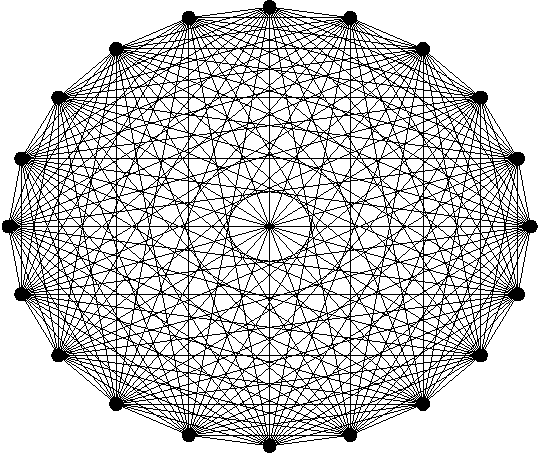
\includegraphics{unnamed-chunk-23-1.pdf}

\begin{center}\rule{0.5\linewidth}{\linethickness}\end{center}

The same 100000 \(M\) matrices were used to investigate stability when
applying each of these different distributions of \(\gamma\) values. The
table below shows the number of \(M\) that were unstable (\_unst) and
stable (\_stbl) for the exponential (Exp), beta, and gamma
distributions.

\begin{Shaded}
\begin{Highlighting}[]
\NormalTok{fourdists <-}\StringTok{ }\KeywordTok{read.csv}\NormalTok{(}\DataTypeTok{file =} \StringTok{"sim_results/different_distr/four_distr_rand.csv"}\NormalTok{);}
\KeywordTok{kable}\NormalTok{(fourdists);}
\end{Highlighting}
\end{Shaded}

\begin{longtable}[]{@{}lllllll@{}}
\toprule
S & Exp\_unst & Exp\_stbl & beta\_unst & beta\_stbl & gamma\_unst &
gamma\_stbl\tabularnewline
\midrule
\endhead
2 & 30 & 99970 & 30 & 99970 & 30 & 99970\tabularnewline
3 & 355 & 99645 & 355 & 99645 & 355 & 99645\tabularnewline
4 & 1506 & 98494 & 1512 & 98488 & 1516 & 98484\tabularnewline
5 & 3930 & 96070 & 3971 & 96029 & 4006 & 95994\tabularnewline
6 & 7738 & 92262 & 7844 & 92156 & 7918 & 92082\tabularnewline
7 & 13606 & 86394 & 13889 & 86111 & 13990 & 86010\tabularnewline
8 & 20535 & 79465 & 21002 & 78998 & 21114 & 78886\tabularnewline
9 & 28614 & 71386 & 29060 & 70940 & 29110 & 70890\tabularnewline
10 & 38375 & 61625 & 38388 & 61612 & 38441 & 61559\tabularnewline
11 & 48616 & 51384 & 48211 & 51789 & 47957 & 52043\tabularnewline
12 & 59254 & 40746 & 58025 & 41975 & 57473 & 42527\tabularnewline
13 & 68816 & 31184 & 66753 & 33247 & 66127 & 33873\tabularnewline
14 & 77721 & 22279 & 75149 & 24851 & 74222 & 25778\tabularnewline
15 & 84842 & 15158 & 82030 & 17970 & 81040 & 18960\tabularnewline
16 & 90365 & 9635 & 87809 & 12191 & 86600 & 13400\tabularnewline
17 & 94171 & 5829 & 91756 & 8244 & 90668 & 9332\tabularnewline
18 & 96978 & 3022 & 94977 & 5023 & 94176 & 5824\tabularnewline
19 & 98376 & 1624 & 97018 & 2982 & 96268 & 3732\tabularnewline
20 & 99218 & 782 & 98357 & 1643 & 97765 & 2235\tabularnewline
21 & 99678 & 322 & 99124 & 876 & 98746 & 1254\tabularnewline
22 & 99864 & 136 & 99599 & 401 & 99323 & 677\tabularnewline
23 & 99954 & 46 & 99783 & 217 & 99668 & 332\tabularnewline
24 & 99978 & 22 & 99920 & 80 & 99821 & 179\tabularnewline
25 & 99996 & 4 & 99967 & 33 & 99911 & 89\tabularnewline
26 & 99999 & 1 & 99979 & 21 & 99960 & 40\tabularnewline
27 & 99999 & 1 & 99990 & 10 & 99983 & 17\tabularnewline
28 & 100000 & 0 & 99999 & 1 & 99991 & 9\tabularnewline
29 & 100000 & 0 & 99999 & 1 & 99999 & 1\tabularnewline
30 & 100000 & 0 & 100000 & 0 & 100000 & 0\tabularnewline
31 & 100000 & 0 & 100000 & 0 & 99999 & 1\tabularnewline
32 & 100000 & 0 & 100000 & 0 & 100000 & 0\tabularnewline
\ldots{} & \ldots{} & \ldots{} & \ldots{} & \ldots{} & \ldots{} &
\ldots{}\tabularnewline
50 & 100000 & 0 & 100000 & 0 & 100000 & 0\tabularnewline
\bottomrule
\end{longtable}

In comparison to the uniform distribution (a), proportionally fewer
random systems are found with the exponential distribution (b), while
more are found with the beta (c) and gamma (d) distributions.

\hypertarget{ga}{\section{Genetic algorithm}\label{ga}}

Ideally, to investigate the potential of \(Var(\gamma)\) for increasing
the proportion of stable complex systems, the search space of all
possible \(\gamma\) vectors would be evaluated for each unique \(M\).
This is technically impossible because \(\gamma_{i}\) can take any real
value between 0-2, but even rounding \(\gamma\) to reasonable values
would result in a search space too large to practically explore. Under
these conditions, genetic algorithms are highly useful tools for finding
practical solutions by mimicking the process of biological
evolution\textsuperscript{\protect\hyperlink{ref-Hamblin2013}{6}}. In
this case, the practical solution is finding vectors of \(\gamma\) that
decrease the most positive real eigenvalue of \(M\). The genetic
algorithm below achieves this by initialising a large population of 1000
different potential \(\gamma\) vectors and allowing this population to
evolve through a process of mutation, crossover (swaping \(\gamma_{i}\)
values between vectors), selection, and reproduction until either a
\(\gamma\) vector is found where all \(\Re(\lambda) < 0\) or some
``giving up'' critiera is met (in the below, this ``giving up''"
criteria is met when 20 generations pass, or if the fitness increase
from one generation to the next is below a certain criteria). The
genetic algorithm relies on five functions. The first outer function
\texttt{Evo\_rand\_gen\_var} runs all of the simulations
(\texttt{max\_sp} refers to the maximum \(S\) value simulated, and
\texttt{iters} refers to the number of \(M\) to try for each \(S\)).

\begin{Shaded}
\begin{Highlighting}[]
\NormalTok{Evo_rand_gen_var <-}\StringTok{ }\NormalTok{function(max_sp, iters, }\DataTypeTok{int_type =} \DecValTok{0}\NormalTok{, }\DataTypeTok{rmx =} \FloatTok{0.4}\NormalTok{, }\DataTypeTok{C =} \DecValTok{1}\NormalTok{)\{}
    \NormalTok{tot_res <-}\StringTok{ }\OtherTok{NULL}\NormalTok{;}
    \NormalTok{fea_res <-}\StringTok{ }\OtherTok{NULL}\NormalTok{;}
    \NormalTok{for(i in }\DecValTok{2}\NormalTok{:max_sp)\{}
        \NormalTok{nn             <-}\StringTok{ }\NormalTok{i;}
        \NormalTok{A1_stt         <-}\StringTok{ }\DecValTok{0}\NormalTok{;}
        \NormalTok{A2_stt         <-}\StringTok{ }\DecValTok{0}\NormalTok{;}
        \NormalTok{A1_fet         <-}\StringTok{ }\DecValTok{0}\NormalTok{;}
        \NormalTok{A2_fet         <-}\StringTok{ }\DecValTok{0}\NormalTok{;}
        \NormalTok{iter           <-}\StringTok{ }\NormalTok{iters;}
        \NormalTok{tot_res[[i}\DecValTok{-1}\NormalTok{]] <-}\StringTok{ }\KeywordTok{matrix}\NormalTok{(}\DataTypeTok{data =} \DecValTok{0}\NormalTok{, }\DataTypeTok{nrow =} \NormalTok{iter, }\DataTypeTok{ncol =} \DecValTok{3}\NormalTok{);}
        \NormalTok{fea_res[[i}\DecValTok{-1}\NormalTok{]] <-}\StringTok{ }\KeywordTok{matrix}\NormalTok{(}\DataTypeTok{data =} \DecValTok{0}\NormalTok{, }\DataTypeTok{nrow =} \NormalTok{iter, }\DataTypeTok{ncol =} \DecValTok{2}\NormalTok{);}
        \NormalTok{while(iter >}\StringTok{ }\DecValTok{0}\NormalTok{)\{}
            \NormalTok{r_vec    <-}\StringTok{ }\KeywordTok{rnorm}\NormalTok{(}\DataTypeTok{n =} \NormalTok{i, }\DataTypeTok{mean =} \DecValTok{0}\NormalTok{, }\DataTypeTok{sd =} \NormalTok{rmx);}
            \NormalTok{A0_dat   <-}\StringTok{ }\KeywordTok{rnorm}\NormalTok{(}\DataTypeTok{n =} \NormalTok{i *}\StringTok{ }\NormalTok{i, }\DataTypeTok{mean =} \DecValTok{0}\NormalTok{, }\DataTypeTok{sd =} \FloatTok{0.4}\NormalTok{);}
            \NormalTok{A0       <-}\StringTok{ }\KeywordTok{matrix}\NormalTok{(}\DataTypeTok{data =} \NormalTok{A0_dat, }\DataTypeTok{nrow =} \NormalTok{i, }\DataTypeTok{ncol =} \NormalTok{i);}
            \NormalTok{A0       <-}\StringTok{ }\KeywordTok{species_interactions}\NormalTok{(}\DataTypeTok{mat =} \NormalTok{A0, }\DataTypeTok{type =} \NormalTok{int_type);}
            \NormalTok{C_dat    <-}\StringTok{ }\KeywordTok{rbinom}\NormalTok{(}\DataTypeTok{n =} \NormalTok{i *}\StringTok{ }\NormalTok{i, }\DataTypeTok{size =} \DecValTok{1}\NormalTok{, }\DataTypeTok{prob =} \NormalTok{C);}
            \NormalTok{C_mat    <-}\StringTok{ }\KeywordTok{matrix}\NormalTok{(}\DataTypeTok{data =} \NormalTok{C_dat, }\DataTypeTok{nrow =} \NormalTok{i, }\DataTypeTok{ncol =} \NormalTok{i);}
            \NormalTok{A0       <-}\StringTok{ }\NormalTok{A0 *}\StringTok{ }\NormalTok{C_mat;}
            \KeywordTok{diag}\NormalTok{(A0) <-}\StringTok{ }\NormalTok{-}\DecValTok{1}\NormalTok{;}
            \NormalTok{gam1     <-}\StringTok{ }\KeywordTok{runif}\NormalTok{(}\DataTypeTok{n =} \NormalTok{i, }\DataTypeTok{min =} \DecValTok{0}\NormalTok{, }\DataTypeTok{max =} \DecValTok{2}\NormalTok{);}
            \NormalTok{A1       <-}\StringTok{ }\NormalTok{A0 *}\StringTok{ }\NormalTok{gam1;}
            \NormalTok{A0_stb   <-}\StringTok{ }\KeywordTok{max}\NormalTok{(}\KeywordTok{Re}\NormalTok{(}\KeywordTok{eigen}\NormalTok{(A0)$values)) <}\StringTok{ }\DecValTok{0}\NormalTok{;}
            \NormalTok{A1_stb   <-}\StringTok{ }\KeywordTok{rand_mat_ga}\NormalTok{(A1);}
            \NormalTok{A0_fea   <-}\StringTok{ }\KeywordTok{min}\NormalTok{(-}\DecValTok{1}\NormalTok{*}\KeywordTok{solve}\NormalTok{(A0) %*%}\StringTok{ }\NormalTok{r_vec) >}\StringTok{ }\DecValTok{0}\NormalTok{;}
            \NormalTok{A1_fea   <-}\StringTok{ }\KeywordTok{min}\NormalTok{(-}\DecValTok{1}\NormalTok{*}\KeywordTok{solve}\NormalTok{(A1) %*%}\StringTok{ }\NormalTok{r_vec) >}\StringTok{ }\DecValTok{0}\NormalTok{;}
            \NormalTok{if(A0_stb ==}\StringTok{ }\OtherTok{TRUE}\NormalTok{)\{}
                \NormalTok{tot_res[[i}\DecValTok{-1}\NormalTok{]][iter, }\DecValTok{1}\NormalTok{] <-}\StringTok{ }\DecValTok{1}\NormalTok{;}
            \NormalTok{\}}
            \NormalTok{if(A1_stb ==}\StringTok{ }\OtherTok{TRUE}\NormalTok{)\{}
                \NormalTok{tot_res[[i}\DecValTok{-1}\NormalTok{]][iter, }\DecValTok{2}\NormalTok{] <-}\StringTok{ }\DecValTok{1}\NormalTok{;}
            \NormalTok{\}}
            \NormalTok{if(A0_fea ==}\StringTok{ }\OtherTok{TRUE}\NormalTok{)\{}
                \NormalTok{fea_res[[i}\DecValTok{-1}\NormalTok{]][iter, }\DecValTok{1}\NormalTok{] <-}\StringTok{ }\DecValTok{1}\NormalTok{;}
            \NormalTok{\}}
            \NormalTok{if(A1_fea ==}\StringTok{ }\OtherTok{TRUE}\NormalTok{)\{}
                \NormalTok{fea_res[[i}\DecValTok{-1}\NormalTok{]][iter, }\DecValTok{2}\NormalTok{] <-}\StringTok{ }\DecValTok{1}\NormalTok{;}
            \NormalTok{\}}
            \NormalTok{iter    <-}\StringTok{ }\NormalTok{iter -}\StringTok{ }\DecValTok{1}\NormalTok{;}
        \NormalTok{\}}
        \KeywordTok{print}\NormalTok{(i);}
    \NormalTok{\}}
    \NormalTok{all_res <-}\StringTok{ }\KeywordTok{summarise_randmat}\NormalTok{(}\DataTypeTok{tot_res =} \NormalTok{tot_res, }\DataTypeTok{fea_res =} \NormalTok{fea_res);}
    \KeywordTok{return}\NormalTok{(all_res);}
\NormalTok{\}}
\end{Highlighting}
\end{Shaded}

Note that \texttt{Evo\_rand\_gen\_var} calls three custom sub-functions,
\texttt{species\_interactions}, \texttt{rand\_mat\_ga}, and
\texttt{summarise\_randmat}. The first simply allows for non-random
interactions between components (e.g., modelling
\protect\hyperlink{ecological}{ecological interactions} of random,
competition, mutualism, or predator-prey).

\begin{Shaded}
\begin{Highlighting}[]
\NormalTok{species_interactions <-}\StringTok{ }\NormalTok{function(mat, }\DataTypeTok{type =} \DecValTok{0}\NormalTok{)\{}
    \NormalTok{if(type ==}\StringTok{ }\DecValTok{1}\NormalTok{)\{}
        \NormalTok{mat[mat >}\StringTok{ }\DecValTok{0}\NormalTok{] <-}\StringTok{ }\NormalTok{-}\DecValTok{1}\NormalTok{*mat[mat >}\StringTok{ }\DecValTok{0}\NormalTok{];}
    \NormalTok{\}}
    \NormalTok{if(type ==}\StringTok{ }\DecValTok{2}\NormalTok{)\{}
        \NormalTok{mat[mat <}\StringTok{ }\DecValTok{0}\NormalTok{] <-}\StringTok{ }\NormalTok{-}\DecValTok{1}\NormalTok{*mat[mat <}\StringTok{ }\DecValTok{0}\NormalTok{];}
    \NormalTok{\}}
    \NormalTok{if(type ==}\StringTok{ }\DecValTok{3}\NormalTok{)\{}
        \NormalTok{for(i in }\DecValTok{1}\NormalTok{:}\KeywordTok{dim}\NormalTok{(mat)[}\DecValTok{1}\NormalTok{])\{}
            \NormalTok{for(j in }\DecValTok{1}\NormalTok{:}\KeywordTok{dim}\NormalTok{(mat)[}\DecValTok{2}\NormalTok{])\{}
                \NormalTok{if(mat[i, j] *}\StringTok{ }\NormalTok{mat[j, i] >}\StringTok{ }\DecValTok{0}\NormalTok{)\{}
                    \NormalTok{mat[j, i] <-}\StringTok{ }\NormalTok{-}\DecValTok{1} \NormalTok{*}\StringTok{ }\NormalTok{mat[j, i];}
                \NormalTok{\}}
            \NormalTok{\}}
        \NormalTok{\}}
    \NormalTok{\}}
    \KeywordTok{return}\NormalTok{(mat);}
\NormalTok{\}}
\end{Highlighting}
\end{Shaded}

The sub-function \texttt{rand\_mat\_ga} does the work of the genetic
algorithm, searching for \(\gamma\) vectors that are stabilising.

\begin{Shaded}
\begin{Highlighting}[]
\NormalTok{rand_mat_ga <-}\StringTok{ }\NormalTok{function(A1, }\DataTypeTok{max_it =} \DecValTok{20}\NormalTok{, }\DataTypeTok{converg =} \FloatTok{0.01}\NormalTok{)\{}
    \NormalTok{nn       <-}\StringTok{ }\KeywordTok{dim}\NormalTok{(A1)[}\DecValTok{1}\NormalTok{];}
    \NormalTok{rind     <-}\StringTok{ }\KeywordTok{runif}\NormalTok{(}\DataTypeTok{n =} \NormalTok{nn*}\DecValTok{1000}\NormalTok{, }\DataTypeTok{min =} \DecValTok{0}\NormalTok{, }\DataTypeTok{max =} \DecValTok{1}\NormalTok{);}
    \NormalTok{inds     <-}\StringTok{ }\KeywordTok{matrix}\NormalTok{(}\DataTypeTok{data =} \NormalTok{rind, }\DataTypeTok{nrow =} \DecValTok{1000}\NormalTok{, }\DataTypeTok{ncol =} \NormalTok{nn);}
    \NormalTok{lastf    <-}\StringTok{ }\NormalTok{-}\DecValTok{10}\NormalTok{;}
    \NormalTok{ccrit    <-}\StringTok{ }\DecValTok{10}\NormalTok{;}
    \NormalTok{find_st  <-}\StringTok{ }\DecValTok{0}\NormalTok{;}
    \NormalTok{iter     <-}\StringTok{ }\NormalTok{max_it;}
    \NormalTok{while(iter >}\StringTok{ }\DecValTok{0} \NormalTok{&}\StringTok{ }\NormalTok{find_st <}\StringTok{ }\DecValTok{1} \NormalTok{&}\StringTok{ }\NormalTok{ccrit >}\StringTok{ }\NormalTok{converg)\{}
        \NormalTok{ivar  <-}\StringTok{ }\KeywordTok{rep}\NormalTok{(}\DataTypeTok{x =} \DecValTok{0}\NormalTok{, }\DataTypeTok{length =} \KeywordTok{dim}\NormalTok{(inds)[}\DecValTok{1}\NormalTok{]);}
        \NormalTok{ifit  <-}\StringTok{ }\KeywordTok{rep}\NormalTok{(}\DataTypeTok{x =} \DecValTok{0}\NormalTok{, }\DataTypeTok{length =} \KeywordTok{dim}\NormalTok{(inds)[}\DecValTok{1}\NormalTok{]);}
        \NormalTok{isst  <-}\StringTok{ }\KeywordTok{rep}\NormalTok{(}\DataTypeTok{x =} \DecValTok{0}\NormalTok{, }\DataTypeTok{length =} \KeywordTok{dim}\NormalTok{(inds)[}\DecValTok{1}\NormalTok{]);}
        \NormalTok{for(i in }\DecValTok{1}\NormalTok{:}\KeywordTok{dim}\NormalTok{(inds)[}\DecValTok{1}\NormalTok{])\{}
            \NormalTok{ifit[i] <-}\StringTok{ }\NormalTok{-}\DecValTok{1}\NormalTok{*}\KeywordTok{max}\NormalTok{(}\KeywordTok{Re}\NormalTok{(}\KeywordTok{eigen}\NormalTok{(inds[i,]*A1)$values));}
            \NormalTok{ivar[i] <-}\StringTok{ }\KeywordTok{var}\NormalTok{(inds[i,]);}
            \NormalTok{isst[i] <-}\StringTok{ }\KeywordTok{max}\NormalTok{(}\KeywordTok{Re}\NormalTok{(}\KeywordTok{eigen}\NormalTok{(inds[i,]*A1)$values)) <}\StringTok{ }\DecValTok{0}\NormalTok{;}
        \NormalTok{\}}
        \NormalTok{most_fit <-}\StringTok{ }\KeywordTok{order}\NormalTok{(ifit, }\DataTypeTok{decreasing =} \OtherTok{TRUE}\NormalTok{)[}\DecValTok{1}\NormalTok{:}\DecValTok{20}\NormalTok{];}
        \NormalTok{parents  <-}\StringTok{ }\NormalTok{inds[most_fit,];}
        \NormalTok{new_gen  <-}\StringTok{ }\KeywordTok{matrix}\NormalTok{(}\DataTypeTok{data =} \KeywordTok{t}\NormalTok{(parents), }\DataTypeTok{nrow =} \DecValTok{1000}\NormalTok{, }\DataTypeTok{ncol =} \NormalTok{nn, }
                           \DataTypeTok{byrow =} \OtherTok{TRUE}\NormalTok{);}
        \NormalTok{mu_dat   <-}\StringTok{ }\KeywordTok{rbinom}\NormalTok{(}\DataTypeTok{n =} \NormalTok{nn*}\DecValTok{1000}\NormalTok{, }\DataTypeTok{size =} \DecValTok{1}\NormalTok{, }\DataTypeTok{prob =} \FloatTok{0.2}\NormalTok{);}
        \NormalTok{mu_dat2  <-}\StringTok{ }\KeywordTok{rnorm}\NormalTok{(}\DataTypeTok{n =} \NormalTok{nn*}\DecValTok{1000}\NormalTok{, }\DataTypeTok{mean =} \DecValTok{0}\NormalTok{, }\DataTypeTok{sd =} \FloatTok{0.02}\NormalTok{);}
        \NormalTok{mu_dat2[mu_dat2 <}\StringTok{ }\DecValTok{0}\NormalTok{] <-}\StringTok{ }\NormalTok{-mu_dat2[mu_dat2 <}\StringTok{ }\DecValTok{0}\NormalTok{];}
        \NormalTok{mu_dat2[mu_dat2 >}\StringTok{ }\DecValTok{2}\NormalTok{] <-}\StringTok{ }\DecValTok{2}\NormalTok{;}
        \NormalTok{mu_dat3  <-}\StringTok{ }\NormalTok{mu_dat *}\StringTok{ }\NormalTok{mu_dat2;}
        \NormalTok{mu_mat   <-}\StringTok{ }\KeywordTok{matrix}\NormalTok{(}\DataTypeTok{data =} \NormalTok{mu_dat3, }\DataTypeTok{nrow =} \DecValTok{1000}\NormalTok{, }\DataTypeTok{ncol =} \NormalTok{nn);}
        \NormalTok{new_gen  <-}\StringTok{ }\NormalTok{new_gen +}\StringTok{ }\NormalTok{mu_mat;}
        \NormalTok{new_gen  <-}\StringTok{ }\KeywordTok{crossover}\NormalTok{(}\DataTypeTok{inds =} \NormalTok{new_gen, }\DataTypeTok{pr =} \FloatTok{0.1}\NormalTok{);}
        \NormalTok{inds     <-}\StringTok{ }\NormalTok{new_gen;}
        \NormalTok{find_st  <-}\StringTok{ }\KeywordTok{max}\NormalTok{(isst);}
        \NormalTok{newf     <-}\StringTok{ }\KeywordTok{mean}\NormalTok{(ifit);}
        \NormalTok{ccrit    <-}\StringTok{ }\NormalTok{newf -}\StringTok{ }\NormalTok{lastf;}
        \NormalTok{lastf    <-}\StringTok{ }\NormalTok{newf;}
        \NormalTok{iter     <-}\StringTok{ }\NormalTok{iter -}\StringTok{ }\DecValTok{1}\NormalTok{;}
    \NormalTok{\}}
    \NormalTok{if(find_st ==}\StringTok{ }\DecValTok{1}\NormalTok{)\{}
        \NormalTok{s_row <-}\StringTok{ }\KeywordTok{which}\NormalTok{(isst ==}\StringTok{ }\DecValTok{1}\NormalTok{)[}\DecValTok{1}\NormalTok{];}
        \NormalTok{writt <-}\StringTok{ }\KeywordTok{c}\NormalTok{(nn, inds[s_row,]);}
        \KeywordTok{cat}\NormalTok{(writt, }\DataTypeTok{file =} \StringTok{"evo_out.txt"}\NormalTok{, }\DataTypeTok{append =} \OtherTok{TRUE}\NormalTok{);}
        \KeywordTok{cat}\NormalTok{(}\StringTok{"}\CharTok{\textbackslash{}n}\StringTok{"}\NormalTok{, }\DataTypeTok{file =} \StringTok{"evo_out.txt"}\NormalTok{, }\DataTypeTok{append =} \OtherTok{TRUE}\NormalTok{);}
    \NormalTok{\}}
    \KeywordTok{return}\NormalTok{(find_st);}
\NormalTok{\}}
\end{Highlighting}
\end{Shaded}

The while loop in \texttt{rand\_mat\_ga} continues until either
\texttt{iter} generations have occured, a solution \(\gamma\) vector is
found that results in all \(\Re(\lambda) < 0\), or some criteria of
minimum fitness increase is observed (by default,
\texttt{converg\ =\ 0.01}). Within the genetic algorithm, \(\gamma\)
values are mutated, crossover occurs between \(\gamma\) vectors, and
selection occurs in each generation such that the 20 \(\gamma\) vectors
that produce the lowest maximum \(\Re(\lambda)\) are allowed to have 50
offspring each. In mutation, any \(\gamma_{i}\) values that mutate below
zero are multiplied by \(-1\), and any values that mutate above 2 are
set to 2. Note also that if a solution is found, then one such
\(\gamma\) vector causing stability is printed to a file.

Crossover occurs in the \texttt{crossover} function below.

\begin{Shaded}
\begin{Highlighting}[]
\NormalTok{crossover <-}\StringTok{ }\NormalTok{function(inds, }\DataTypeTok{pr =} \FloatTok{0.1}\NormalTok{)\{}
    \NormalTok{crossed <-}\StringTok{ }\KeywordTok{floor}\NormalTok{(}\KeywordTok{dim}\NormalTok{(inds)[}\DecValTok{1}\NormalTok{] *}\StringTok{ }\NormalTok{pr);}
    \NormalTok{cross1  <-}\StringTok{ }\KeywordTok{sample}\NormalTok{(}\DataTypeTok{x =} \DecValTok{1}\NormalTok{:}\KeywordTok{dim}\NormalTok{(inds)[}\DecValTok{1}\NormalTok{], }\DataTypeTok{size =} \NormalTok{crossed);}
    \NormalTok{cross2  <-}\StringTok{ }\KeywordTok{sample}\NormalTok{(}\DataTypeTok{x =} \DecValTok{1}\NormalTok{:}\KeywordTok{dim}\NormalTok{(inds)[}\DecValTok{1}\NormalTok{], }\DataTypeTok{size =} \NormalTok{crossed);}
    \NormalTok{for(i in }\DecValTok{1}\NormalTok{:}\KeywordTok{length}\NormalTok{(cross1))\{}
        \NormalTok{fromv   <-}\StringTok{ }\KeywordTok{sample}\NormalTok{(}\DataTypeTok{x =} \DecValTok{1}\NormalTok{:}\KeywordTok{dim}\NormalTok{(inds)[}\DecValTok{2}\NormalTok{], }\DataTypeTok{size =} \DecValTok{1}\NormalTok{);}
        \NormalTok{tov     <-}\StringTok{ }\KeywordTok{sample}\NormalTok{(}\DataTypeTok{x =} \DecValTok{1}\NormalTok{:}\KeywordTok{dim}\NormalTok{(inds)[}\DecValTok{2}\NormalTok{], }\DataTypeTok{size =} \DecValTok{1}\NormalTok{);}
        \NormalTok{temp                   <-}\StringTok{ }\NormalTok{inds[cross1[i],fromv:tov];}
        \NormalTok{inds[cross1[i],fromv:tov] <-}\StringTok{ }\NormalTok{inds[cross2[i],fromv:tov];}
        \NormalTok{inds[cross2[i],fromv:tov] <-}\StringTok{ }\NormalTok{temp;}
    \NormalTok{\}}
    \KeywordTok{return}\NormalTok{(inds);}
\NormalTok{\}}
\end{Highlighting}
\end{Shaded}

After all \(M\) are simulated in \texttt{Evo\_rand\_gen\_var}, the
\texttt{summarise\_randmat} formats the data into a table.

\begin{Shaded}
\begin{Highlighting}[]
\NormalTok{summarise_randmat_ga <-}\StringTok{ }\NormalTok{function(tot_res, fea_res)\{}
    \NormalTok{sims    <-}\StringTok{ }\KeywordTok{length}\NormalTok{(tot_res);}
    \NormalTok{all_res <-}\StringTok{ }\KeywordTok{matrix}\NormalTok{(}\DataTypeTok{data =} \DecValTok{0}\NormalTok{, }\DataTypeTok{nrow =} \NormalTok{sims, }\DataTypeTok{ncol =} \DecValTok{10}\NormalTok{);}
    \NormalTok{for(i in }\DecValTok{1}\NormalTok{:sims)\{}
        \NormalTok{unstables <-}\StringTok{ }\NormalTok{tot_res[[i]][,}\DecValTok{1}\NormalTok{] ==}\StringTok{ }\OtherTok{FALSE} \NormalTok{&}\StringTok{ }\NormalTok{tot_res[[i]][,}\DecValTok{2}\NormalTok{] ==}\StringTok{ }\OtherTok{FALSE}\NormalTok{;}
        \NormalTok{stables   <-}\StringTok{ }\NormalTok{tot_res[[i]][,}\DecValTok{1}\NormalTok{] ==}\StringTok{ }\OtherTok{TRUE}  \NormalTok{&}\StringTok{ }\NormalTok{tot_res[[i]][,}\DecValTok{2}\NormalTok{] ==}\StringTok{ }\OtherTok{TRUE}\NormalTok{;}
        \NormalTok{unstabled <-}\StringTok{ }\NormalTok{tot_res[[i]][,}\DecValTok{1}\NormalTok{] ==}\StringTok{ }\OtherTok{TRUE}  \NormalTok{&}\StringTok{ }\NormalTok{tot_res[[i]][,}\DecValTok{2}\NormalTok{] ==}\StringTok{ }\OtherTok{FALSE}\NormalTok{;}
        \NormalTok{stabled   <-}\StringTok{ }\NormalTok{tot_res[[i]][,}\DecValTok{1}\NormalTok{] ==}\StringTok{ }\OtherTok{FALSE} \NormalTok{&}\StringTok{ }\NormalTok{tot_res[[i]][,}\DecValTok{2}\NormalTok{] ==}\StringTok{ }\OtherTok{TRUE}\NormalTok{;}
        \NormalTok{non_feas  <-}\StringTok{ }\NormalTok{fea_res[[i]][,}\DecValTok{1}\NormalTok{] ==}\StringTok{ }\OtherTok{FALSE} \NormalTok{&}\StringTok{ }\NormalTok{fea_res[[i]][,}\DecValTok{2}\NormalTok{] ==}\StringTok{ }\OtherTok{FALSE}\NormalTok{;}
        \NormalTok{feasibl   <-}\StringTok{ }\NormalTok{fea_res[[i]][,}\DecValTok{1}\NormalTok{] ==}\StringTok{ }\OtherTok{TRUE}  \NormalTok{&}\StringTok{ }\NormalTok{fea_res[[i]][,}\DecValTok{2}\NormalTok{] ==}\StringTok{ }\OtherTok{TRUE}\NormalTok{;}
        \NormalTok{unfeased  <-}\StringTok{ }\NormalTok{fea_res[[i]][,}\DecValTok{1}\NormalTok{] ==}\StringTok{ }\OtherTok{TRUE}  \NormalTok{&}\StringTok{ }\NormalTok{fea_res[[i]][,}\DecValTok{2}\NormalTok{] ==}\StringTok{ }\OtherTok{FALSE}\NormalTok{;}
        \NormalTok{feased    <-}\StringTok{ }\NormalTok{fea_res[[i]][,}\DecValTok{1}\NormalTok{] ==}\StringTok{ }\OtherTok{FALSE} \NormalTok{&}\StringTok{ }\NormalTok{fea_res[[i]][,}\DecValTok{2}\NormalTok{] ==}\StringTok{ }\OtherTok{TRUE}\NormalTok{;}
        \NormalTok{foundd    <-}\StringTok{ }\NormalTok{tot_res[[i]][,}\DecValTok{3}\NormalTok{] ==}\StringTok{ }\OtherTok{TRUE}\NormalTok{;}
        \NormalTok{all_res[i, }\DecValTok{1}\NormalTok{]  <-}\StringTok{ }\NormalTok{i +}\StringTok{ }\DecValTok{1}\NormalTok{;}
        \NormalTok{all_res[i, }\DecValTok{2}\NormalTok{]  <-}\StringTok{ }\KeywordTok{sum}\NormalTok{(unstables);}
        \NormalTok{all_res[i, }\DecValTok{3}\NormalTok{]  <-}\StringTok{ }\KeywordTok{sum}\NormalTok{(stables);}
        \NormalTok{all_res[i, }\DecValTok{4}\NormalTok{]  <-}\StringTok{ }\KeywordTok{sum}\NormalTok{(unstabled);}
        \NormalTok{all_res[i, }\DecValTok{5}\NormalTok{]  <-}\StringTok{ }\KeywordTok{sum}\NormalTok{(stabled);}
        \NormalTok{all_res[i, }\DecValTok{6}\NormalTok{]  <-}\StringTok{ }\KeywordTok{sum}\NormalTok{(non_feas);}
        \NormalTok{all_res[i, }\DecValTok{7}\NormalTok{]  <-}\StringTok{ }\KeywordTok{sum}\NormalTok{(feasibl);}
        \NormalTok{all_res[i, }\DecValTok{8}\NormalTok{]  <-}\StringTok{ }\KeywordTok{sum}\NormalTok{(unfeased);}
        \NormalTok{all_res[i, }\DecValTok{9}\NormalTok{]  <-}\StringTok{ }\KeywordTok{sum}\NormalTok{(feased);}
        \NormalTok{all_res[i, }\DecValTok{10}\NormalTok{] <-}\StringTok{ }\KeywordTok{sum}\NormalTok{(foundd);}
    \NormalTok{\}}
    \KeywordTok{return}\NormalTok{(all_res);}
\NormalTok{\}}
\end{Highlighting}
\end{Shaded}

Some stability results from this table are shown below. Results for \texttt{A0}
indicate systems in which \(\gamma = 1\), while \texttt{A1} refers to systems in 
which the genetic algorithm searched for a set of \(\gamma\) values that 
stabilised the system. 

\begin{longtable}[]{@{}rrrrrrr@{}}
\toprule
N & A0\_unstable & A0\_stable & A1\_unstable & A1\_stable &
A1\_stabilised & A1\_destabilised\tabularnewline
\midrule
\endhead
2 & 4 & 9996 & 4 & 9996 & 0 & 0\tabularnewline
3 & 42 & 9958 & 42 & 9958 & 0 & 0\tabularnewline
4 & 133 & 9867 & 133 & 9867 & 0 & 0\tabularnewline
5 & 414 & 9586 & 411 & 9589 & 3 & 0\tabularnewline
6 & 809 & 9191 & 799 & 9201 & 10 & 0\tabularnewline
7 & 1380 & 8620 & 1339 & 8661 & 41 & 0\tabularnewline
8 & 2074 & 7926 & 1927 & 8073 & 147 & 0\tabularnewline
9 & 2885 & 7115 & 2503 & 7497 & 382 & 0\tabularnewline
10 & 3842 & 6158 & 3158 & 6842 & 684 & 0\tabularnewline
11 & 4867 & 5133 & 3613 & 6387 & 1255 & 1\tabularnewline
12 & 5932 & 4068 & 4148 & 5852 & 1784 & 0\tabularnewline
13 & 6937 & 3063 & 4470 & 5530 & 2468 & 1\tabularnewline
14 & 7784 & 2216 & 4724 & 5276 & 3060 & 0\tabularnewline
15 & 8519 & 1481 & 5086 & 4914 & 3433 & 0\tabularnewline
16 & 9081 & 919 & 5262 & 4738 & 3819 & 0\tabularnewline
17 & 9431 & 569 & 5368 & 4632 & 4063 & 0\tabularnewline
18 & 9671 & 329 & 5571 & 4429 & 4100 & 0\tabularnewline
19 & 9844 & 156 & 5807 & 4193 & 4037 & 0\tabularnewline
20 & 9934 & 66 & 6133 & 3867 & 3801 & 0\tabularnewline
21 & 6387 & 34 & 6421 & 3579 & 3545 & 0\tabularnewline
22 & 6634 & 11 & 6645 & 3355 & 3344 & 0\tabularnewline
23 & 7037 & 8 & 7045 & 2955 & 2947 & 0\tabularnewline
24 & 7468 & 3 & 7471 & 2529 & 2526 & 0\tabularnewline
25 & 7816 & 0 & 7816 & 2184 & 2184 & 0\tabularnewline
26 & 8192 & 0 & 8192 & 1808 & 1808 & 0\tabularnewline
27 & 8680 & 0 & 8680 & 1320 & 1320 & 0\tabularnewline
28 & 8936 & 0 & 8936 & 1064 & 1064 & 0\tabularnewline
29 & 9296 & 0 & 9296 & 704 & 704 & 0\tabularnewline
30 & 9523 & 0 & 9523 & 477 & 477 & 0\tabularnewline
31 & 9705 & 0 & 9705 & 295 & 295 & 0\tabularnewline
32 & 9816 & 0 & 9816 & 184 & 184 & 0\tabularnewline
33 & 9894 & 0 & 9894 & 106 & 106 & 0\tabularnewline
34 & 9941 & 0 & 9941 & 59 & 59 & 0\tabularnewline
35 & 9968 & 0 & 9968 & 32 & 32 & 0\tabularnewline
36 & 9991 & 0 & 9991 & 9 & 9 & 0\tabularnewline
37 & 9993 & 0 & 9993 & 7 & 7 & 0\tabularnewline
38 & 9999 & 0 & 9999 & 1 & 1 & 0\tabularnewline
39 & 9999 & 0 & 9999 & 1 & 1 & 0\tabularnewline
40 & 10000 & 0 & 10000 & 0 & 0 & 0\tabularnewline
\bottomrule
\end{longtable}

The distributions of nine \(\gamma\) vectors from the highest \(S\)
values are shown below. Recall that 1 million random matrices were
generated for the less computationally intense task of
\protect\hyperlink{IncrS}{comparing} \(M\) when \(\gamma = 1\) versus
when \(\gamma \sim \mathcal{U}(0, 2)\), so it is more informative to
compare stability in column 5 above with column 3 above. \textbf{This
comparison shows the high number of stable \(M\) that can be produced
through a targetted search of \(\gamma\) values, and suggests that many
otherwise unstable systems could potentially be stabilised by an
informed manipulation of their component response times. Such a
possibility might conceivably reduce the dimensionality of problems
involving stability in social-ecological or economic systems.}

Distributions of \(\gamma\) values in vectors for the highest values of
\(S\) are shown below.

\begin{Shaded}
\begin{Highlighting}[]
\NormalTok{evo_out <-}\StringTok{ }\KeywordTok{scan}\NormalTok{(}\DataTypeTok{file =} \StringTok{"sim_results/evolved/evo_out.txt"}\NormalTok{);}
\KeywordTok{plot_evo_out}\NormalTok{(evo_out);}
\end{Highlighting}
\end{Shaded}

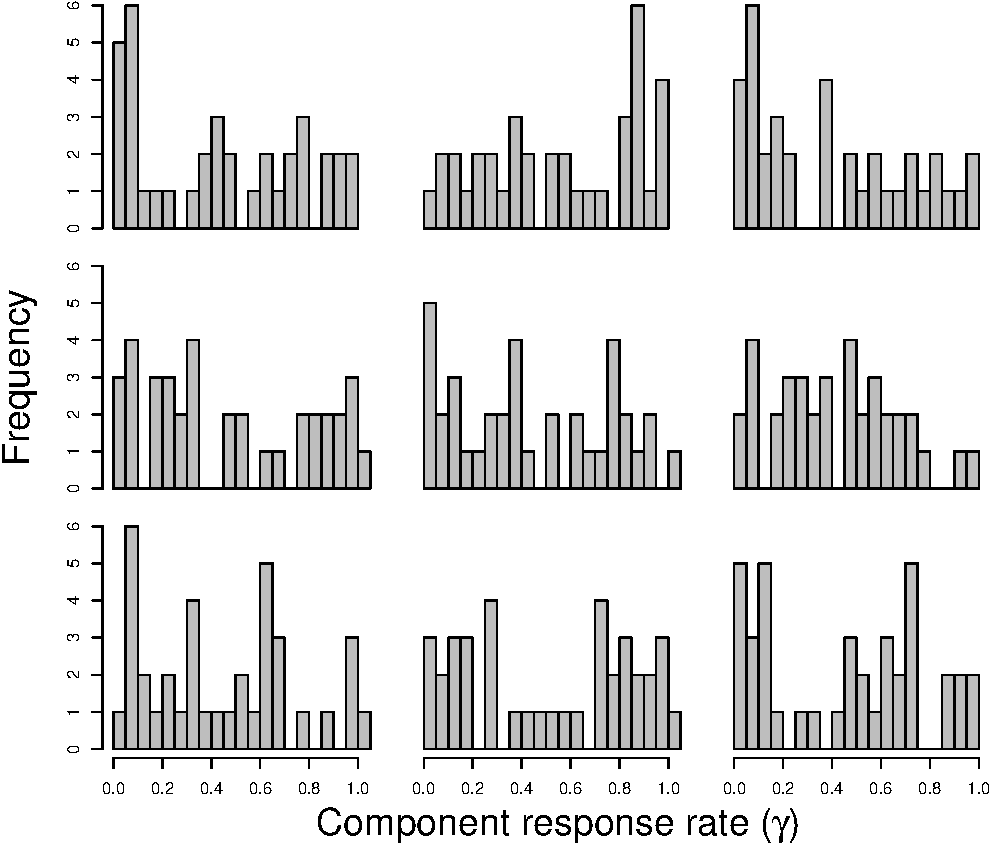
\includegraphics{unnamed-chunk-31-1.pdf}

The distribution of \(\gamma\) values found by the genetic algorithm is
uniform. A uniform distribution was used to initialise \(\gamma\)
values, so there is therefore no evidence that a particular distribution
of \(\gamma\) is likely to be found to stabilise a matrix \(M\).

\hypertarget{Feasibility}{\section{Feasibility of complex
systems}\label{Feasibility}}

For complex systems in which individual system components (\(S\))
represent the density of some tangible quantity, it is important to
consider the feasibility of the system. Feasibile equilibria assume that
the values of all system components are positive at
equilibrium\textsuperscript{\protect\hyperlink{ref-Grilli2017}{7}--\protect\hyperlink{ref-Song2018}{9}}.
This is of particular interest for ecological communities because
population density cannot take negative values, meaning that ecological
systems need to be feasible for stability to be biologically
realistic\textsuperscript{\protect\hyperlink{ref-Dougoud2018}{8}}.
Consequently, the use of random matrices and traditional stability
critiera for making inferences in theoretical analyses of species
networks has recently been
criticised\textsuperscript{\protect\hyperlink{ref-Dougoud2018}{8}}.
While the key results in the main text are intended to be general to all
complex systems, and not restricted to species networks, I have also
performed a feasibility analysis on all matrices \(M\). This analysis
reveals that feasibility is not affected by \(Var(\gamma)\), meaning
that for pure interacting species networks, variation in component
response time (i.e., species generation time) does not affect stability
at biologically realistic species densities. Nevertheless, ecological
interactions do not exist in isolation in empirical systems, but instead
interact with
evolutionary\textsuperscript{\protect\hyperlink{ref-Patel2018}{10}},
abiotic, or social-economic systems. The relevance of \(\gamma\) for
complex system stability presented in the main text should therefore not
be ignored in the broader context of ecological communities.

Dougoud et al.\textsuperscript{\protect\hyperlink{ref-Dougoud2018}{8}}
define the following feasibility criteria for ecological systems
characterised by \(S\) interacting species with varying densities.

\[x^{*} = -\left(\theta I + (CS)^{-\delta}A\right)^{-1}r.\]

In the above, \(x^{*}\) is the vector of species abundances at
equilibrium (for feasibility, all values in \(x^{*}\) must be positive).
The matrix \(I\) is the identity matrix (1s on the diagonal, 0s on the
off-diagonal elements), and the value \(\theta\) is strength of
intraspecific competition (diagonal elements). As I have done elsewhere,
diagonal values are set to \(-1\), so \(\theta = -1\). The variable
\(C\) is the connectance of the community,
which was set to \(C = 1\) throughout the manuscript and supplemental
information, except \protect\hyperlink{connectance}{where otherwise
noted}. The variable \(\delta\) is a normalisation parameter that
modulates the strength of interactions (\(\sigma\) in the main text),
which are held in \(A\). In the main text, implicitly, \(\delta = 0\)
underlying strong interactions. Hence, the whole \((CS)^{-\delta} = 1\),
so in the above, a diagonal matrix of -1s (\(\theta I\)) is added to
\(A\), which has a diagonal of all zeros and an off-diagonal affecting
species interactions (i.e., the expression \((CS)^{-\delta}\) relates to
May's\textsuperscript{\protect\hyperlink{ref-May1972}{1}} stability
criterion\textsuperscript{\protect\hyperlink{ref-Dougoud2018}{8}} by
\(\frac{\sigma}{(CS)^{-\delta}}\sqrt{SC} < -1\), and hence
\((CS)^{-\delta} = 1\) for the randomly simulated systems in the main
text and Supplementary Information). The above criteria is therefore
reduced to the below; note that the parenthetical in both equations
produces an \(M\) matrix as used throughout the main text and
supplemental information,

\[x^{*} = -\left(\theta I + A\right)^{-1}r.\]

To check the feasibility criteria, I therefore inverted
\(M = (\theta I + A)\) and multiplied elements by -1, then multiplied
the resulting matrix by the vector of population growth rates \(r\).
Feasibility is satisfied if all of the elements of the resulting vector
are positive.

The population growth rate for an individual species \(i\) is sampled
from a normal distribution of \(r_{i} \sim \mathcal{N}(0, 0.4^{2})\), as
shown in the \texttt{rand\_gen\_var} function in
\protect\hyperlink{IncrS}{the section} on ``Stability across increasing
\(S\)'' above. Hence, each component \(i\) of the complex system \(M\)
is assumed to be a species with a growth rate of \(r_{i}\). Note that
negative intrinsic growth rates are not unrealistic, and will occur in
obligate mutualists in the absence of a partner.

When feasibility was evaluated with and without variation in \(\gamma\),
there was no increase in stability for \(M\) where \(\gamma\) varied as
compared to where \(\gamma = 1\). Results below illustrate this result,
which was general to all other simulations performed.

\begin{longtable}[]{@{}rrrrrrr@{}}
\toprule
S & A0\_infeasible & A0\_feasible & A1\_infeasible & A1\_feasible &
A1\_made\_feasible & A1\_made\_infeasible\tabularnewline
\midrule
\endhead
2 & 749978 & 250022 & 749942 & 250058 & 35552 & 35516\tabularnewline
3 & 874519 & 125481 & 874296 & 125704 & 36803 & 36580\tabularnewline
4 & 937192 & 62808 & 937215 & 62785 & 26440 & 26463\tabularnewline
5 & 968776 & 31224 & 968639 & 31361 & 16319 & 16182\tabularnewline
6 & 984313 & 15687 & 984463 & 15537 & 9006 & 9156\tabularnewline
7 & 992149 & 7851 & 992161 & 7839 & 4991 & 5003\tabularnewline
8 & 996124 & 3876 & 996103 & 3897 & 2644 & 2623\tabularnewline
9 & 998014 & 1986 & 998027 & 1973 & 1361 & 1374\tabularnewline
10 & 999031 & 969 & 999040 & 960 & 698 & 707\tabularnewline
11 & 999546 & 454 & 999514 & 486 & 377 & 345\tabularnewline
12 & 999764 & 236 & 999792 & 208 & 160 & 188\tabularnewline
13 & 999883 & 117 & 999865 & 135 & 105 & 87\tabularnewline
14 & 999938 & 62 & 999945 & 55 & 40 & 47\tabularnewline
15 & 999971 & 29 & 999964 & 36 & 31 & 24\tabularnewline
16 & 999988 & 12 & 999991 & 9 & 8 & 11\tabularnewline
17 & 999996 & 4 & 999991 & 9 & 8 & 3\tabularnewline
18 & 999997 & 3 & 999999 & 1 & 1 & 3\tabularnewline
19 & 999998 & 2 & 999997 & 3 & 3 & 2\tabularnewline
20 & 1000000 & 0 & 999999 & 1 & 1 & 0\tabularnewline
21 & 1000000 & 0 & 1000000 & 0 & 0 & 0\tabularnewline
22 & 999999 & 1 & 1000000 & 0 & 0 & 1\tabularnewline
23 & 1000000 & 0 & 1000000 & 0 & 0 & 0\tabularnewline
24 & 1000000 & 0 & 1000000 & 0 & 0 & 0\tabularnewline
25 & 1000000 & 0 & 1000000 & 0 & 0 & 0\tabularnewline
26 & 1000000 & 0 & 1000000 & 0 & 0 & 0\tabularnewline
27 & 1000000 & 0 & 1000000 & 0 & 0 & 0\tabularnewline
28 & 1000000 & 0 & 1000000 & 0 & 0 & 0\tabularnewline
29 & 1000000 & 0 & 1000000 & 0 & 0 & 0\tabularnewline
30 & 1000000 & 0 & 1000000 & 0 & 0 & 0\tabularnewline
31 & 1000000 & 0 & 1000000 & 0 & 0 & 0\tabularnewline
32 & 1000000 & 0 & 1000000 & 0 & 0 & 0\tabularnewline
33 & 1000000 & 0 & 1000000 & 0 & 0 & 0\tabularnewline
34 & 1000000 & 0 & 1000000 & 0 & 0 & 0\tabularnewline
35 & 1000000 & 0 & 1000000 & 0 & 0 & 0\tabularnewline
36 & 1000000 & 0 & 1000000 & 0 & 0 & 0\tabularnewline
37 & 1000000 & 0 & 1000000 & 0 & 0 & 0\tabularnewline
38 & 1000000 & 0 & 1000000 & 0 & 0 & 0\tabularnewline
39 & 1000000 & 0 & 1000000 & 0 & 0 & 0\tabularnewline
40 & 1000000 & 0 & 1000000 & 0 & 0 & 0\tabularnewline
41 & 1000000 & 0 & 1000000 & 0 & 0 & 0\tabularnewline
42 & 1000000 & 0 & 1000000 & 0 & 0 & 0\tabularnewline
43 & 1000000 & 0 & 1000000 & 0 & 0 & 0\tabularnewline
44 & 1000000 & 0 & 1000000 & 0 & 0 & 0\tabularnewline
45 & 1000000 & 0 & 1000000 & 0 & 0 & 0\tabularnewline
46 & 1000000 & 0 & 1000000 & 0 & 0 & 0\tabularnewline
47 & 1000000 & 0 & 1000000 & 0 & 0 & 0\tabularnewline
48 & 1000000 & 0 & 1000000 & 0 & 0 & 0\tabularnewline
49 & 1000000 & 0 & 1000000 & 0 & 0 & 0\tabularnewline
50 & 1000000 & 0 & 1000000 & 0 & 0 & 0\tabularnewline
\bottomrule
\end{longtable}

Hence, in general, \(Var(\gamma)\) does not appear to affect feasibility
in pure species interaction networks.

\section*{References}\label{references}
\addcontentsline{toc}{section}{References}

\hypertarget{refs}{}
\hypertarget{ref-Patel2018}{}
1. Patel, S., Cortez, M. H. \& Schreiber, S. J. Partitioning the effects
of eco-evolutionary feedbacks on community stability. \emph{American
Naturalist} \textbf{191,} 1--29 (2018).

\hypertarget{refs}{}
\hypertarget{ref-May1972}{}
2. May, R. M. Will a large complex system be stable? \emph{Nature}
\textbf{238,} 413--414 (1972).

\hypertarget{ref-May1973}{}
3. May, R. M. Qualitative stability in model ecosystems. \emph{Ecology}
\textbf{54,} 638--641 (1973).

\hypertarget{ref-Allesina2012}{}
4. Allesina, S. \& Tang, S. Stability criteria for complex ecosystems.
\emph{Nature} \textbf{483,} 205--208 (2012).

\hypertarget{ref-Allesina2015a}{}
5. Allesina, S. \& Tang, S. The stability--complexity relationship at
age 40: a random matrix perspective. \emph{Population Ecology} 63--75
(2015).
doi:\href{https://doi.org/10.1007/s10144-014-0471-0}{10.1007/s10144-014-0471-0}

\hypertarget{ref-Tang2014b}{}
6. Tang, S. \& Allesina, S. Reactivity and stability of large
ecosystems. \emph{Frontiers in Ecology and Evolution} \textbf{2,} 1--8
(2014).

\hypertarget{ref-Allesina2011}{}
7. Allesina, S. \& Levine, J. M. A competitive network theory of species
diversity. \emph{Proceedings of the National Academy of Sciences of the
United States of America} \textbf{108,} 5638--5642 (2011).

\hypertarget{ref-Hamblin2013}{}
8. Hamblin, S. On the practical usage of genetic algorithms in ecology
and evolution. \emph{Methods in Ecology and Evolution} \textbf{4,}
184--194 (2013).

\hypertarget{ref-Grilli2017}{}
9. Grilli, J. \emph{et al.} Feasibility and coexistence of large
ecological communities. \emph{Nature Communications} \textbf{8,} (2017).

\hypertarget{ref-Dougoud2018}{}
10. Dougoud, M., Vinckenbosch, L., Rohr, R., Bersier, L.-F. \& Mazza, C.
The feasibility of equilibria in large ecosystems: a primary but
neglected concept in the complexity-stability debate. \emph{PLOS
Computational Biology} \textbf{14,} e1005988 (2018).

\hypertarget{ref-Song2018}{}
11. Song, C. \& Saavedra, S. Will a small randomly assembled community be
feasible and stable? \emph{Ecology} \textbf{99,} 743--751 (2018).

\end{document}
